\chapter{Análisis y Resultados}

En este capítulo se describe el proceso de selección de variables a considerar en el estudio,  con las cuales se ejecutará el algoritmo X-Means. Luego se presentan los resultados obtenidos y sus respectivos análisis.

\section{Variables}
Las variables seleccionadas tanto para establecimientos como para las matrículas, que se encuentran individualizadas en los anexos \ref{tab:atributos_establecimientos} y \ref{tab:atributos_matriculas} respectivamente, fueron filtradas según los porcentajes que ocupan cada uno de sus valores. Es decir, se contabilizó la cantidad de repeticiones para un valor dentro de la variable y se calculó su porcentaje. Con esto de clasificaron en 3 categorías según su importancia:


\begin{itemize}
    \item Baja: cuando el porcentaje de aparición de un valor es mayor o igual a 95\%. 
    \item Media: cuando el porcentaje de aparición de un valor es mayor o igual a 85\% y menor que 95\%.
    \item Alta: cuando ni uno de los valores de una variable alcanza un porcentaje de aparición mayor o igual a 85\%.
\end{itemize}

Además de esta categorización se distinguieron las variables propias del establecimiento/matrícula y las que las relacionan. Las de relación para los establecimientos son IDE por rangos, distancia al establecimiento y nivel de sobre edad de sus alumnos. En el caso de las matrículas son distancia al colegio y nivel de copago.

\section{Experimentación}

En primera instancia se ejecutó X-Means para establecimientos y matrículas en 3 diferentes versiones, una con todas las variables, una con las de importancia alta y media, y finalmente una solo con las de alta (todas estas sin considerar las variables que los relacionan). Por tratarse de un aprendizaje no supervisado es difícil establecer una medida de eficiencia  y se tomaron como válidas las siguientes versiones. En el caso de los establecimientos se puede notar en la tabla \ref{tab:cl_estab} que se mantiene constante un clúster de gran tamaño que agrupa casi un 50\% del total de colegios, en donde además en la segunda y tercera versión el resto de los clústers tiene una cardinalidad similar. Considerando lo anterior y el hecho de que al ejecutar el algoritmo con menos variables el tiempo de ejecución es menor, se tomó para estudio la tercera versión que solo considera las variables de alta importancia.

En el caso de las matrículas, como se puede apreciar en la tabla \ref{tab:cl_mat}, los resultados entre las diferentes pruebas son bastante diferentes a nivel de cardinalidad de sus clústers. Por lo tanto, considerando que la tercera prueba genera grupos de similar tamaño y que por tener una menor cantidad de variables se ejecuta en menos tiempo, se utilizó esta versión en el resto del estudio.

\begin{table}[]
\centering
\caption{Clústers de establecimientos. }
\label{tab:cl_estab}
\begin{tabular}{|c|c|c|c|c|}
\hline
\textbf{Variables} & \textbf{E\_TODOS\_0} & \textbf{E\_TODOS\_1} & \textbf{E\_TODOS\_2} & \textbf{E\_TODOS\_3}   \\ \hline
Todas & 959 & 826 & 247 & 36 \\ \hline
Alta + Media & 959 & 540 & 311 & 258 \\ \hline
Alta & 977 & 524 & 308 & 259\\ \hline
\end{tabular}
\end{table}

\begin{table}[]
\centering
\caption{Clústers de matrículas.}
\label{tab:cl_mat}
\begin{tabular}{|c|c|c|c|c|}
\hline
\textbf{Variables} & \textbf{E\_TODOS\_0} & \textbf{E\_TODOS\_1} & \textbf{E\_TODOS\_2} & \textbf{E\_TODOS\_3}   \\ \hline
Todas & 551932 & 442048 & 13585 & 40803 \\ \hline
Alta + Media & 442048 & 551932 & 34088 & 20300 \\ \hline
Alta & 286089 & 300007 & 230486 & 231786 \\ \hline
\end{tabular}
\end{table}

\begin{figure}[h]
 \centering
  \subfloat[Clúster de establecimientos E\_TODOS\_SIN\_0.]{
   \label{f:}
    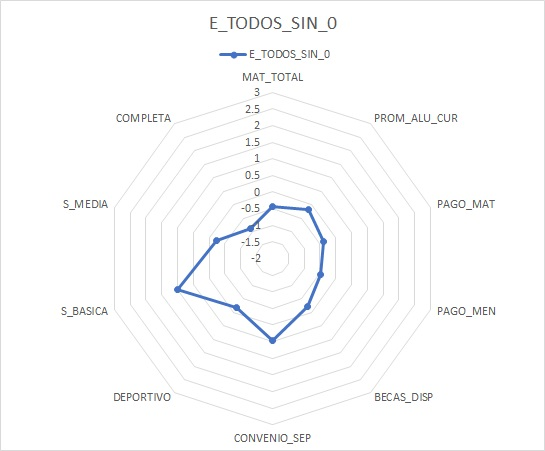
\includegraphics[width=7.5cm]{images/establecimientos/radar_sin_0.jpg}}
  \subfloat[Clúster de establecimientos E\_TODOS\_SIN\_1.]{
   \label{f:}
    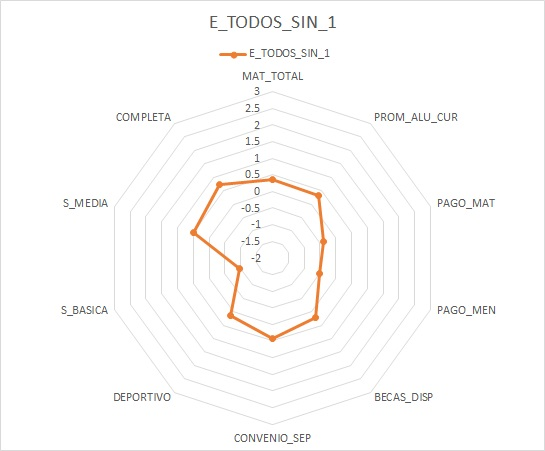
\includegraphics[width=7.5cm]{images/establecimientos/radar_sin_1.jpg}}\hspace{1mm}
  \subfloat[Clúster de establecimientos E\_TODOS\_SIN\_2.]{
   \label{f:}
    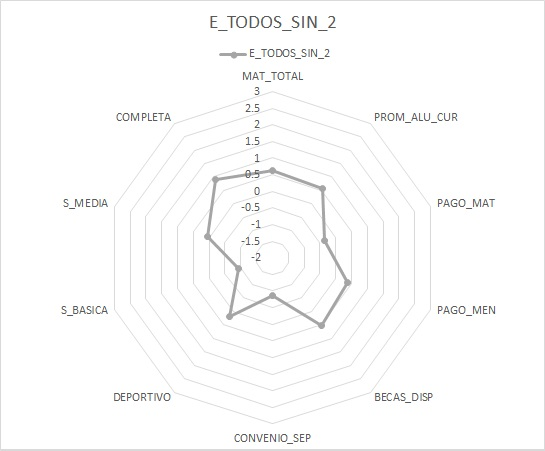
\includegraphics[width=7.5cm]{images/establecimientos/radar_sin_2.jpg}}
  \subfloat[Clúster de establecimientos E\_TODOS\_SIN\_3.]{
   \label{f:}
    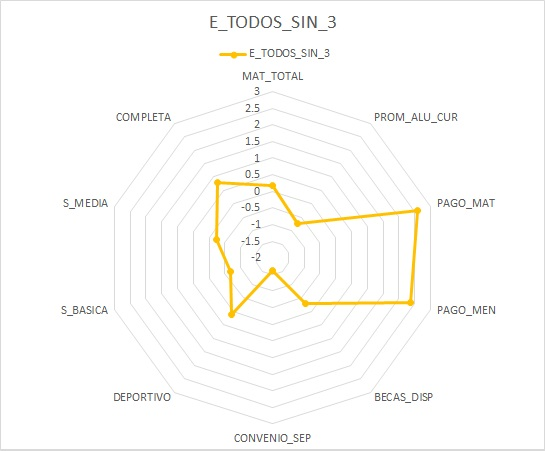
\includegraphics[width=7.5cm]{images/establecimientos/radar_sin_3.jpg}}
 \caption{Promedios de atributos normalizados de establecimientos de la Región Metropolitana.}
 \label{f:}
\end{figure}

\begin{figure}[h]
 \centering
  \subfloat[Clúster de establecimientos E\_TODOS\_CON\_0.]{
   \label{f:}
    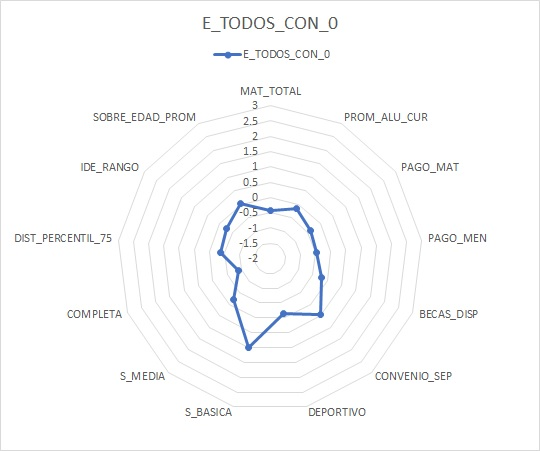
\includegraphics[width=7.5cm]{images/establecimientos/radar_con_0.jpg}}
  \subfloat[Clúster de establecimientos E\_TODOS\_CON\_1.]{
   \label{f:}
    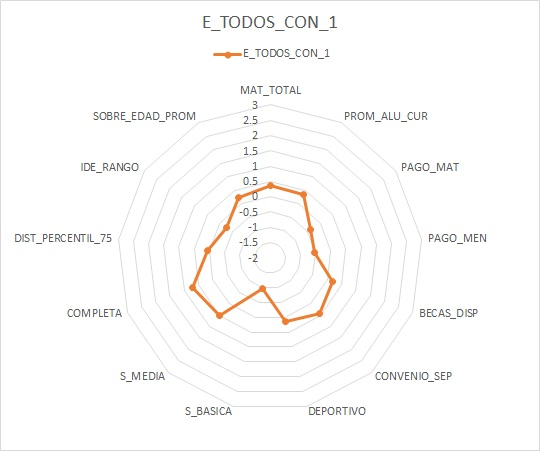
\includegraphics[width=7.5cm]{images/establecimientos/radar_con_1.jpg}}\hspace{1mm}
  \subfloat[Clúster de establecimientos E\_TODOS\_CON\_2.]{
   \label{f:}
    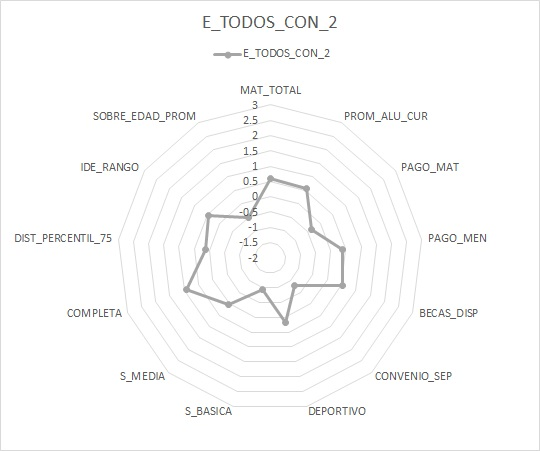
\includegraphics[width=7.5cm]{images/establecimientos/radar_con_2.jpg}}
  \subfloat[Clúster de establecimientos E\_TODOS\_CON\_3.]{
   \label{f:}
    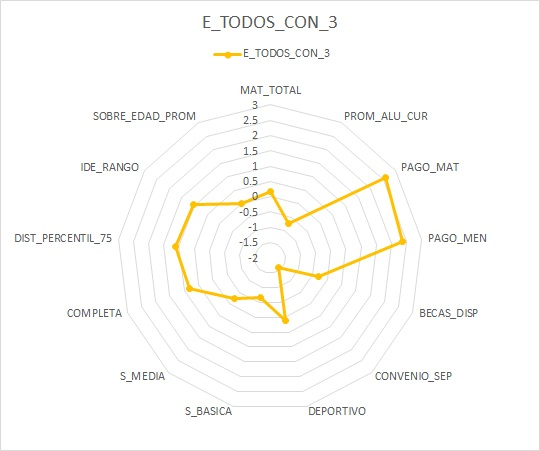
\includegraphics[width=7.5cm]{images/establecimientos/radar_con_3.jpg}}
 \caption{Promedios de atributos normalizados de establecimientos (con atributos relacionales) de la Región Metropolitana.}\
 \label{f:}
\end{figure}

\begin{figure}[h]
 \centering
  \subfloat[Establecimientos clúster E\_TODOS\_SIN\_0.]{
   \label{f:}
    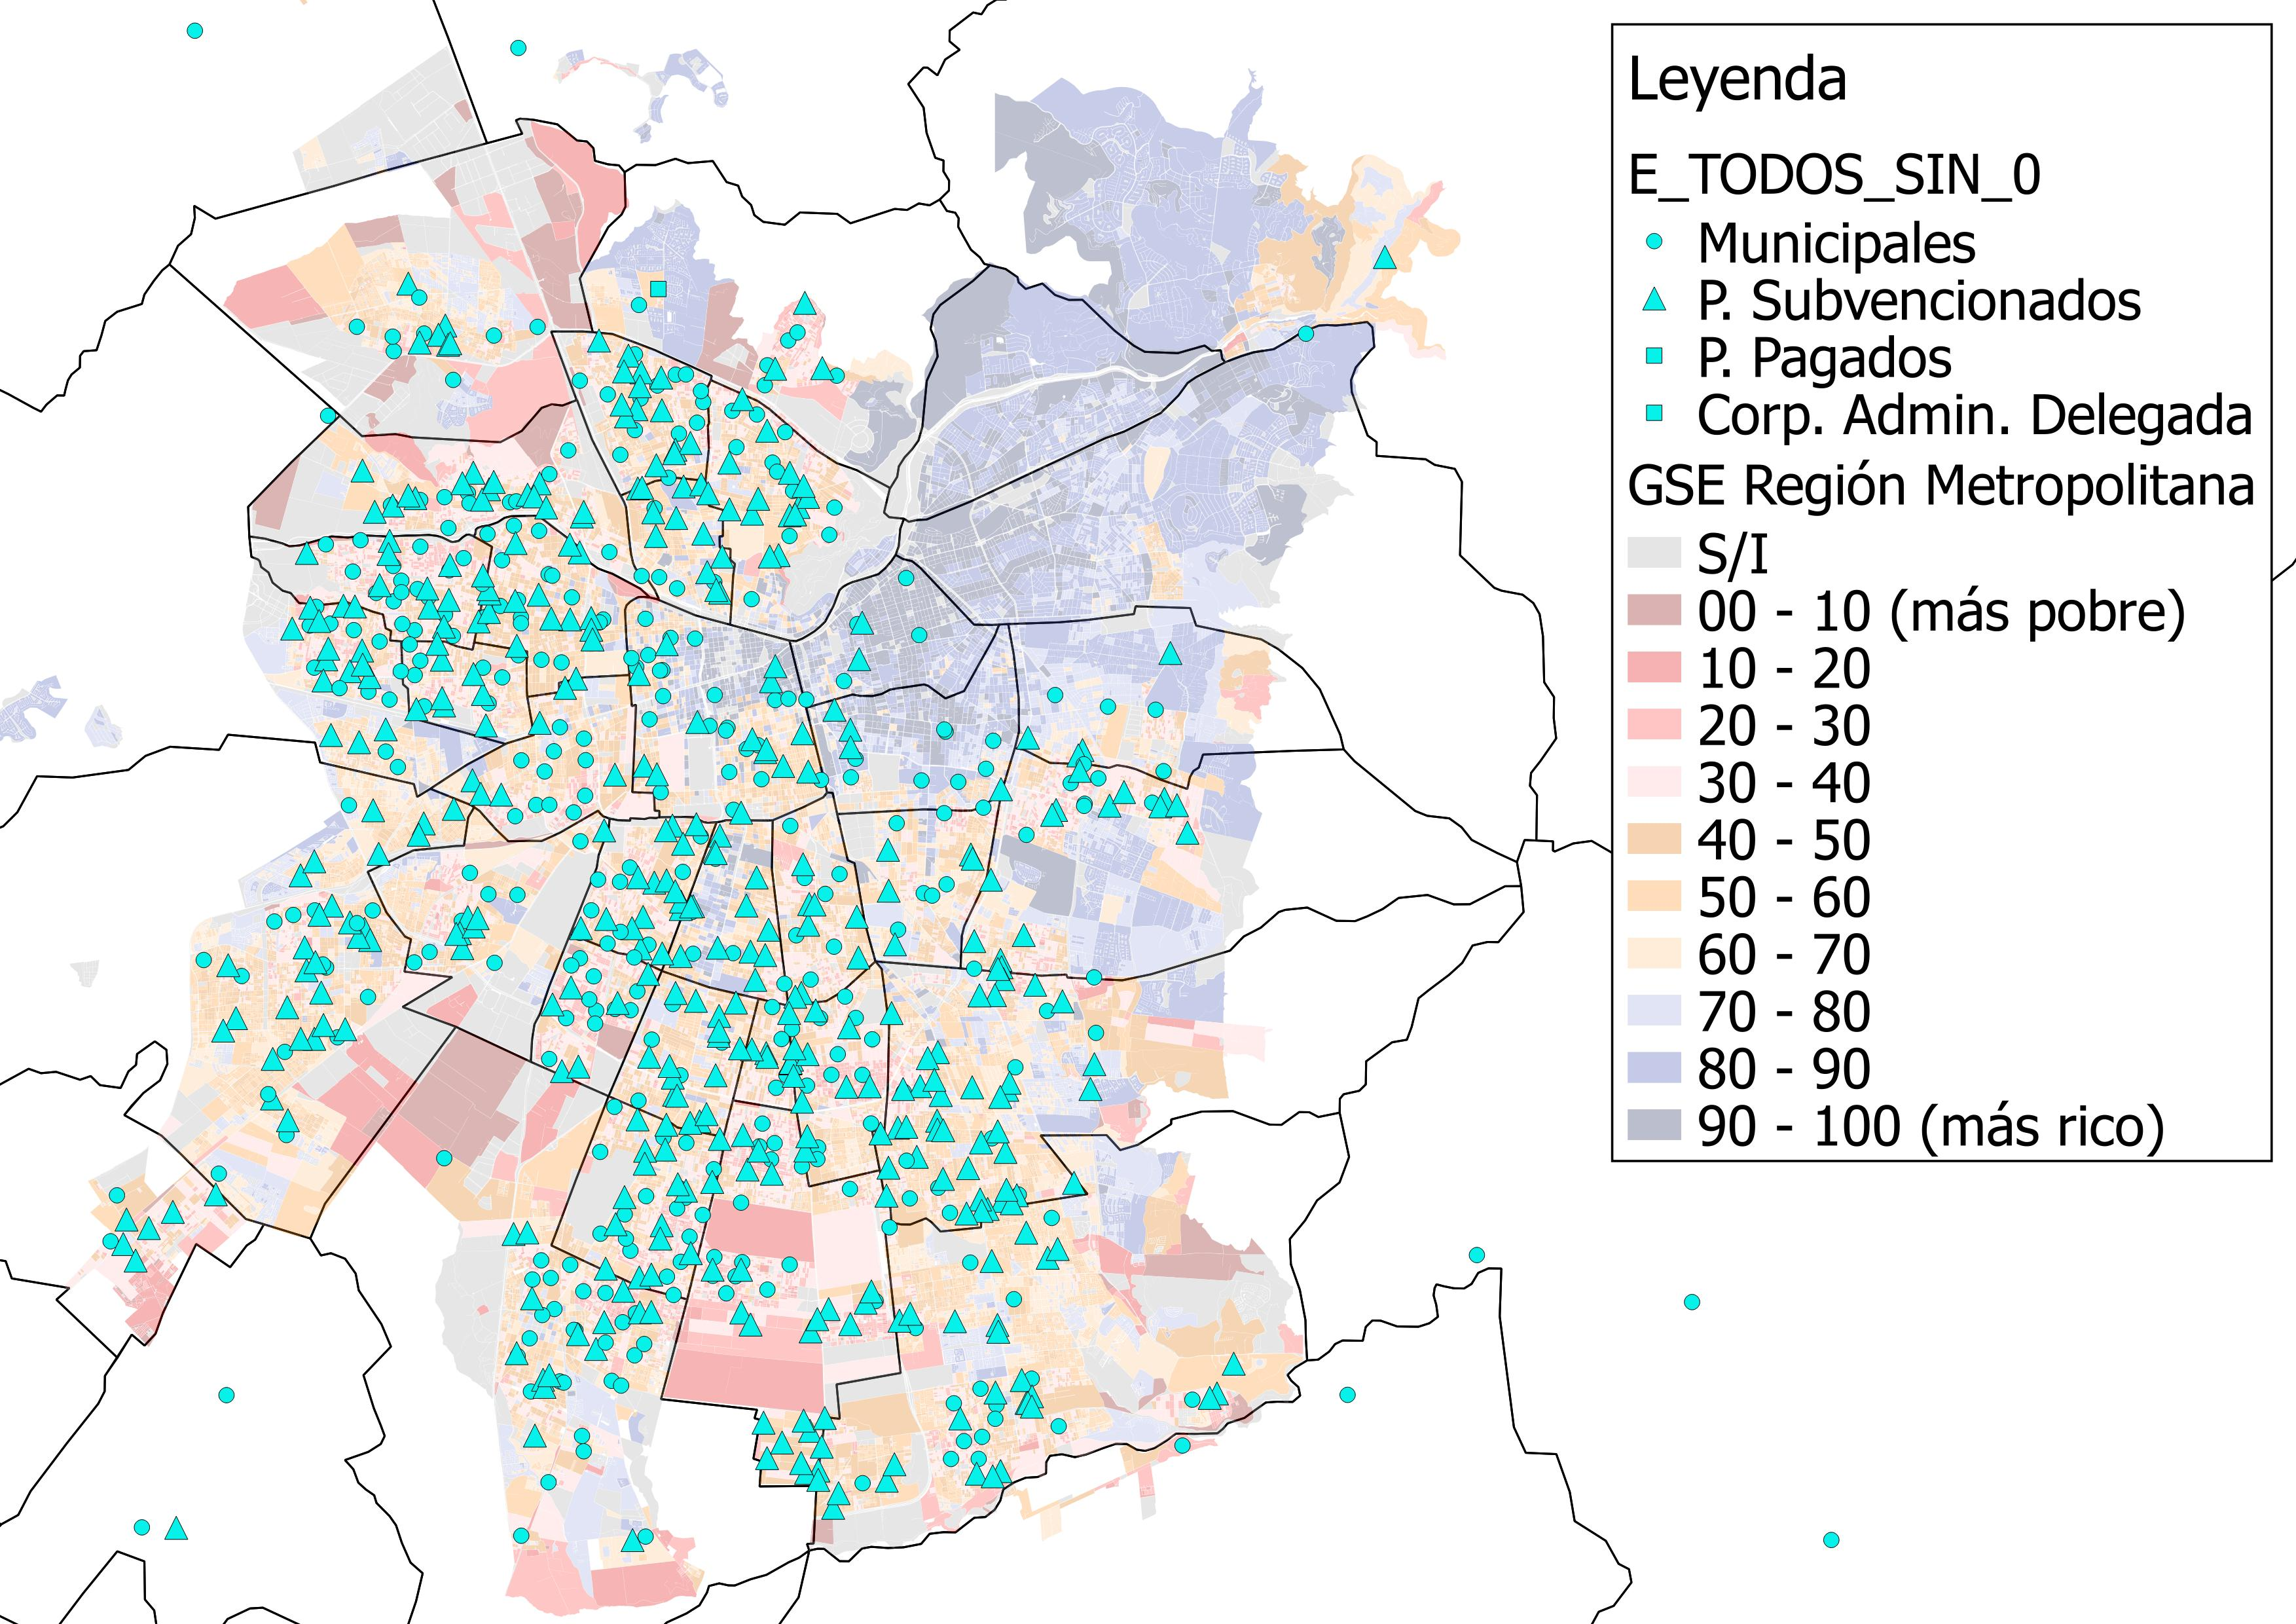
\includegraphics[width=7.5cm]{images/establecimientos/E_TODOS_SIN_0.jpg}}
  \subfloat[Establecimientos clúster E\_TODOS\_SIN\_1.]{
   \label{f:}
    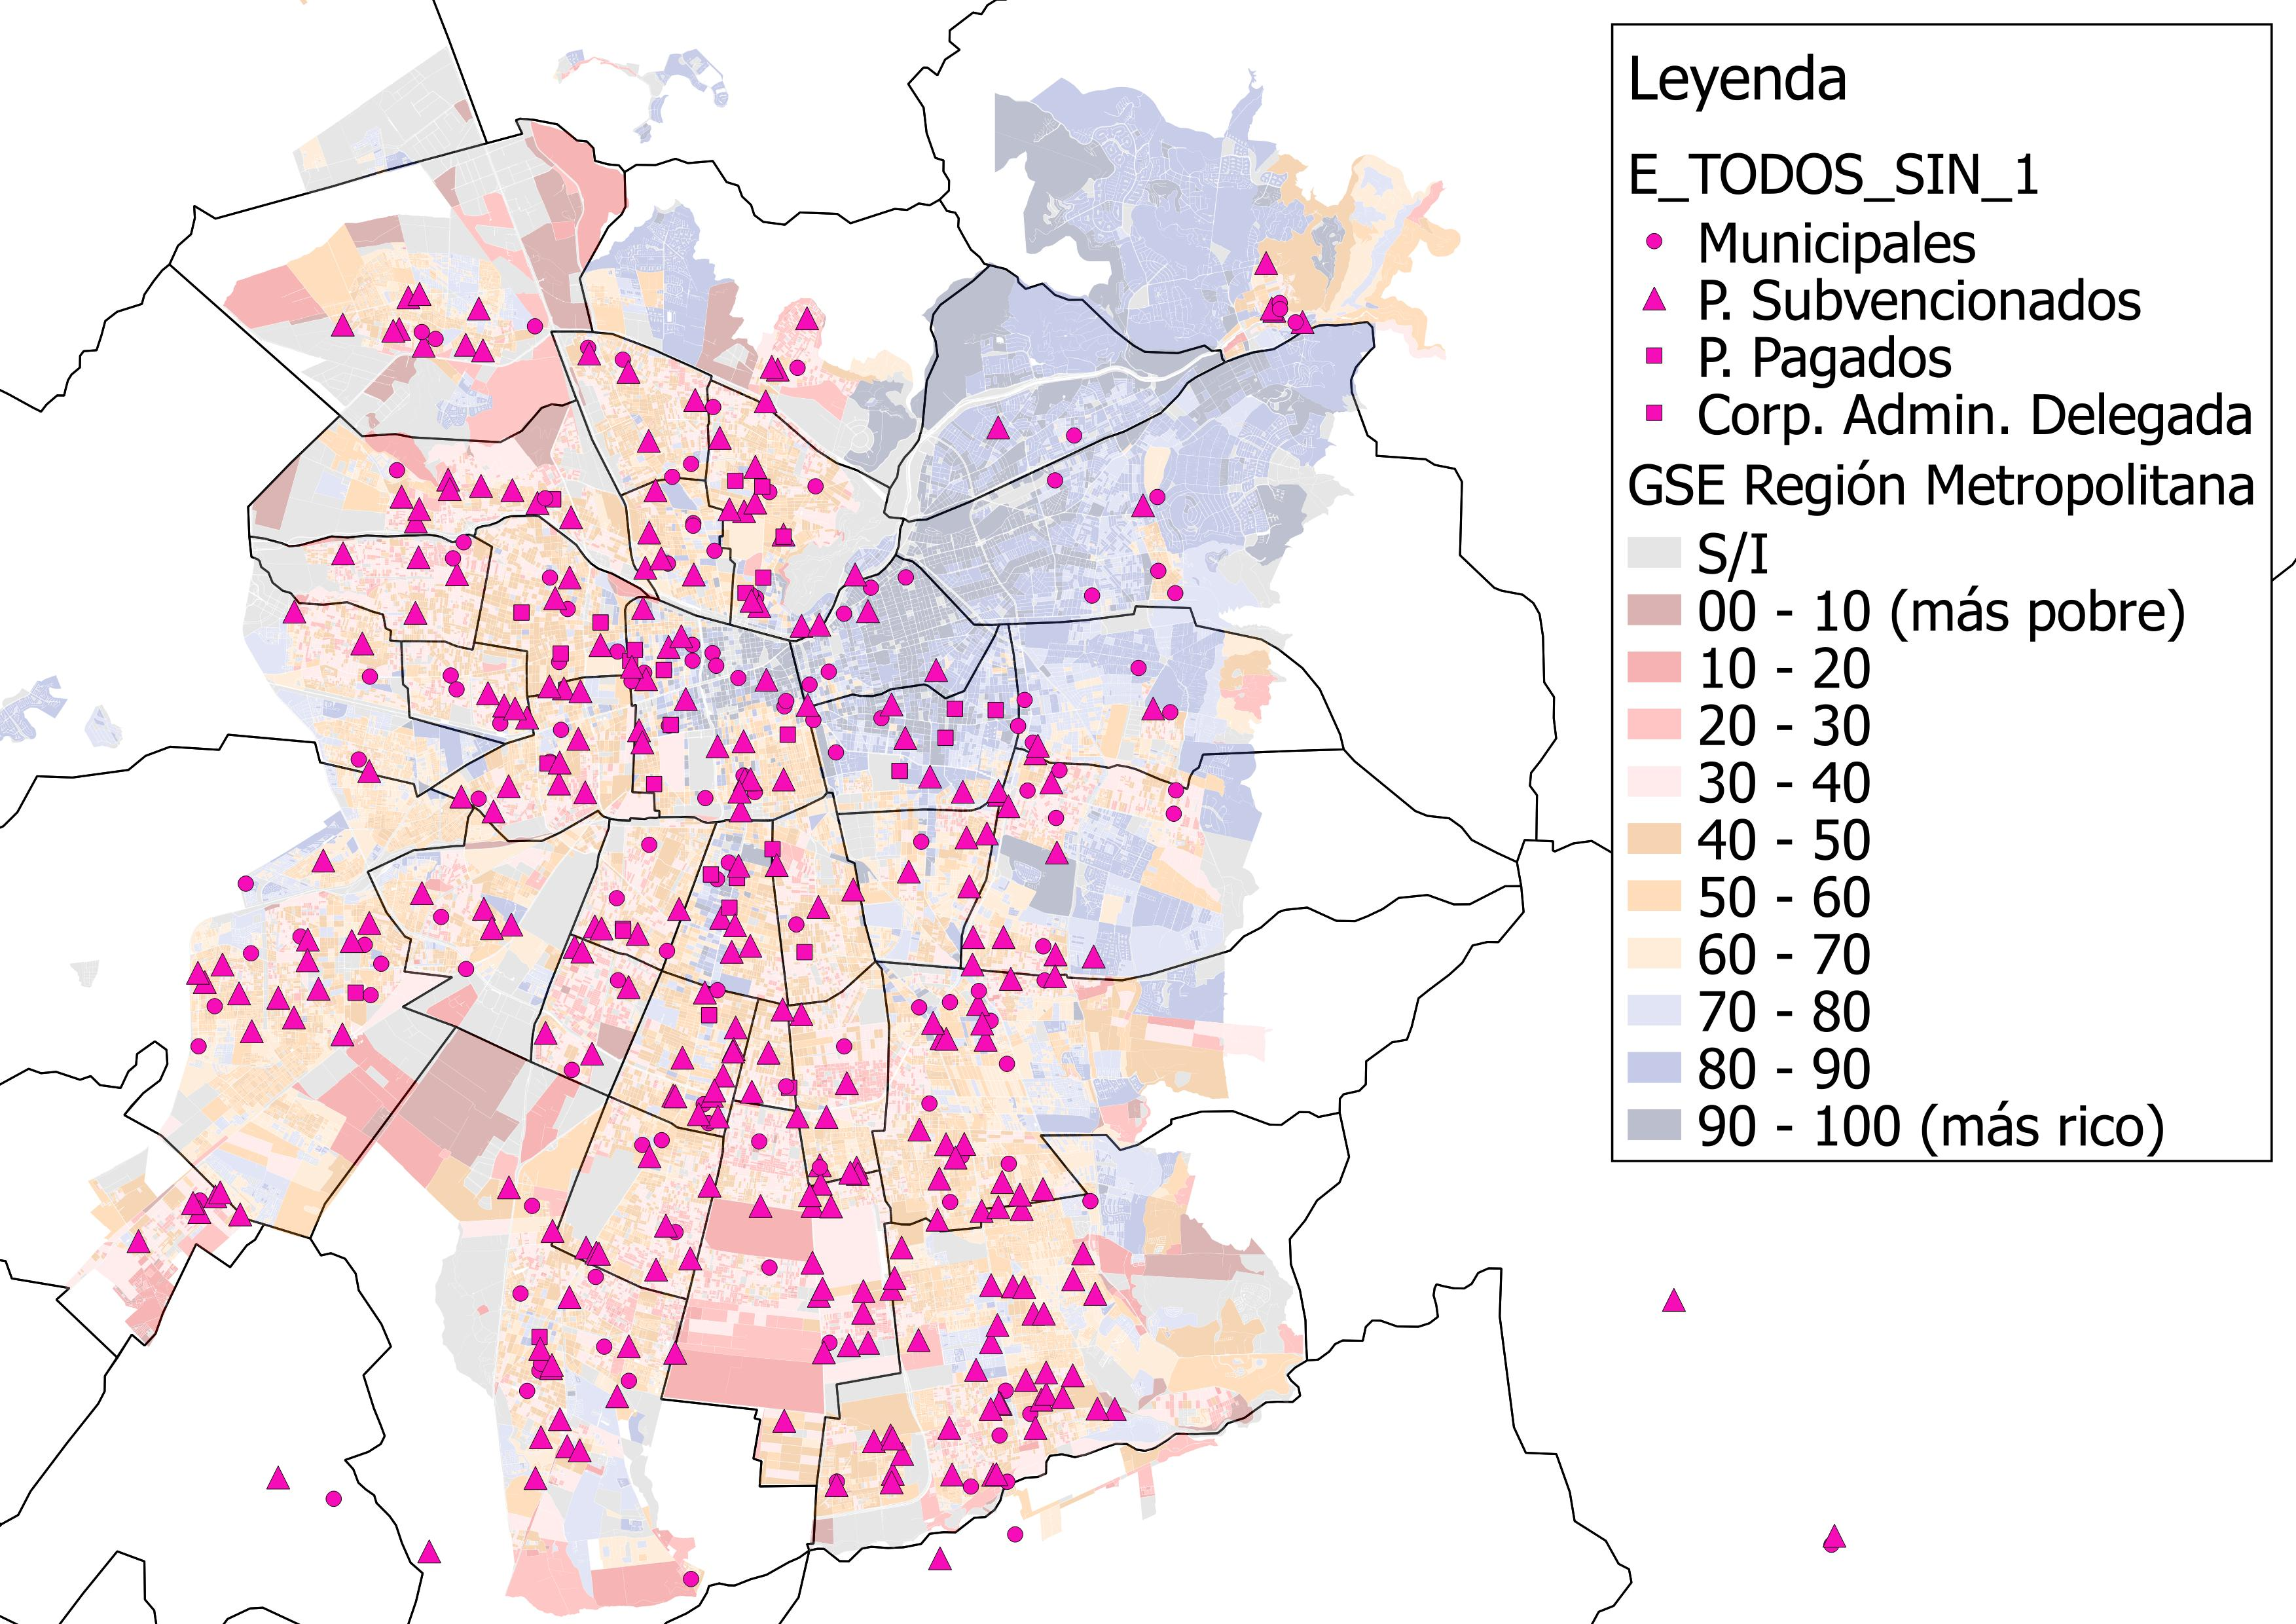
\includegraphics[width=7.5cm]{images/establecimientos/E_TODOS_SIN_1.jpg}}\hspace{1mm}
  \subfloat[Establecimientos clúster E\_TODOS\_SIN\_2.]{
   \label{f:}
    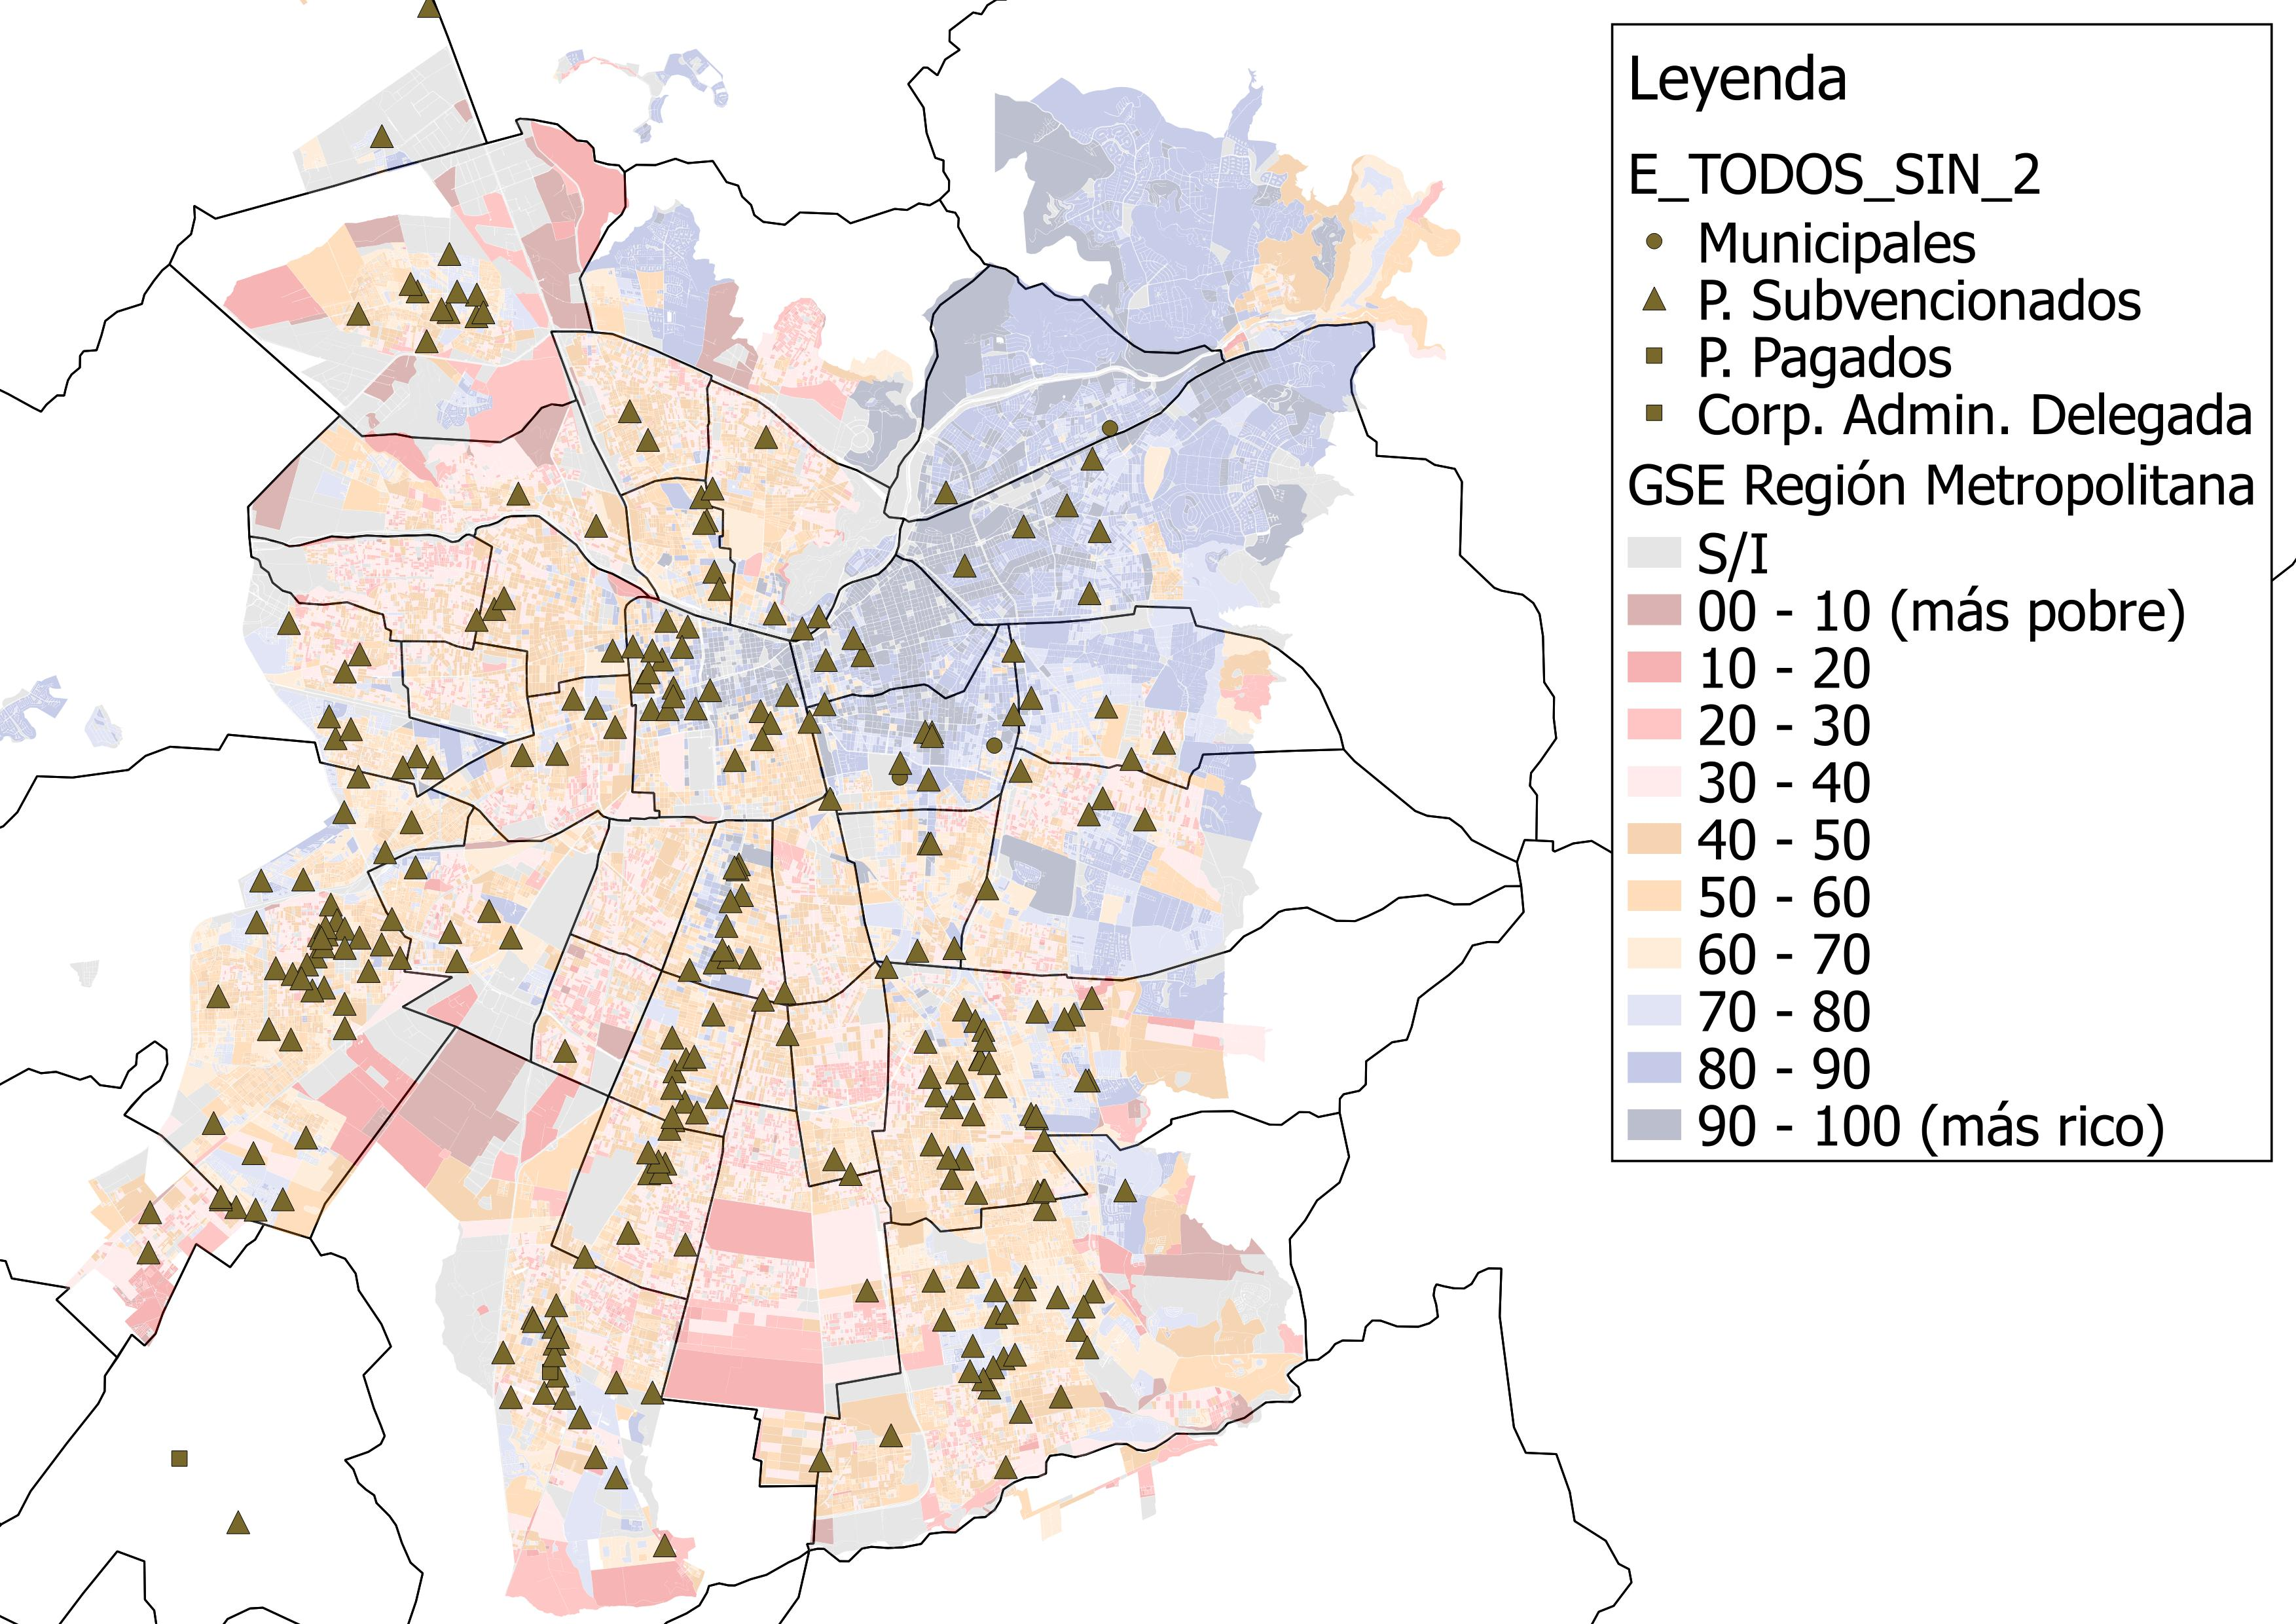
\includegraphics[width=7.5cm]{images/establecimientos/E_TODOS_SIN_2.jpg}}
  \subfloat[Establecimientos clúster E\_TODOS\_SIN\_3.]{
   \label{f:}
    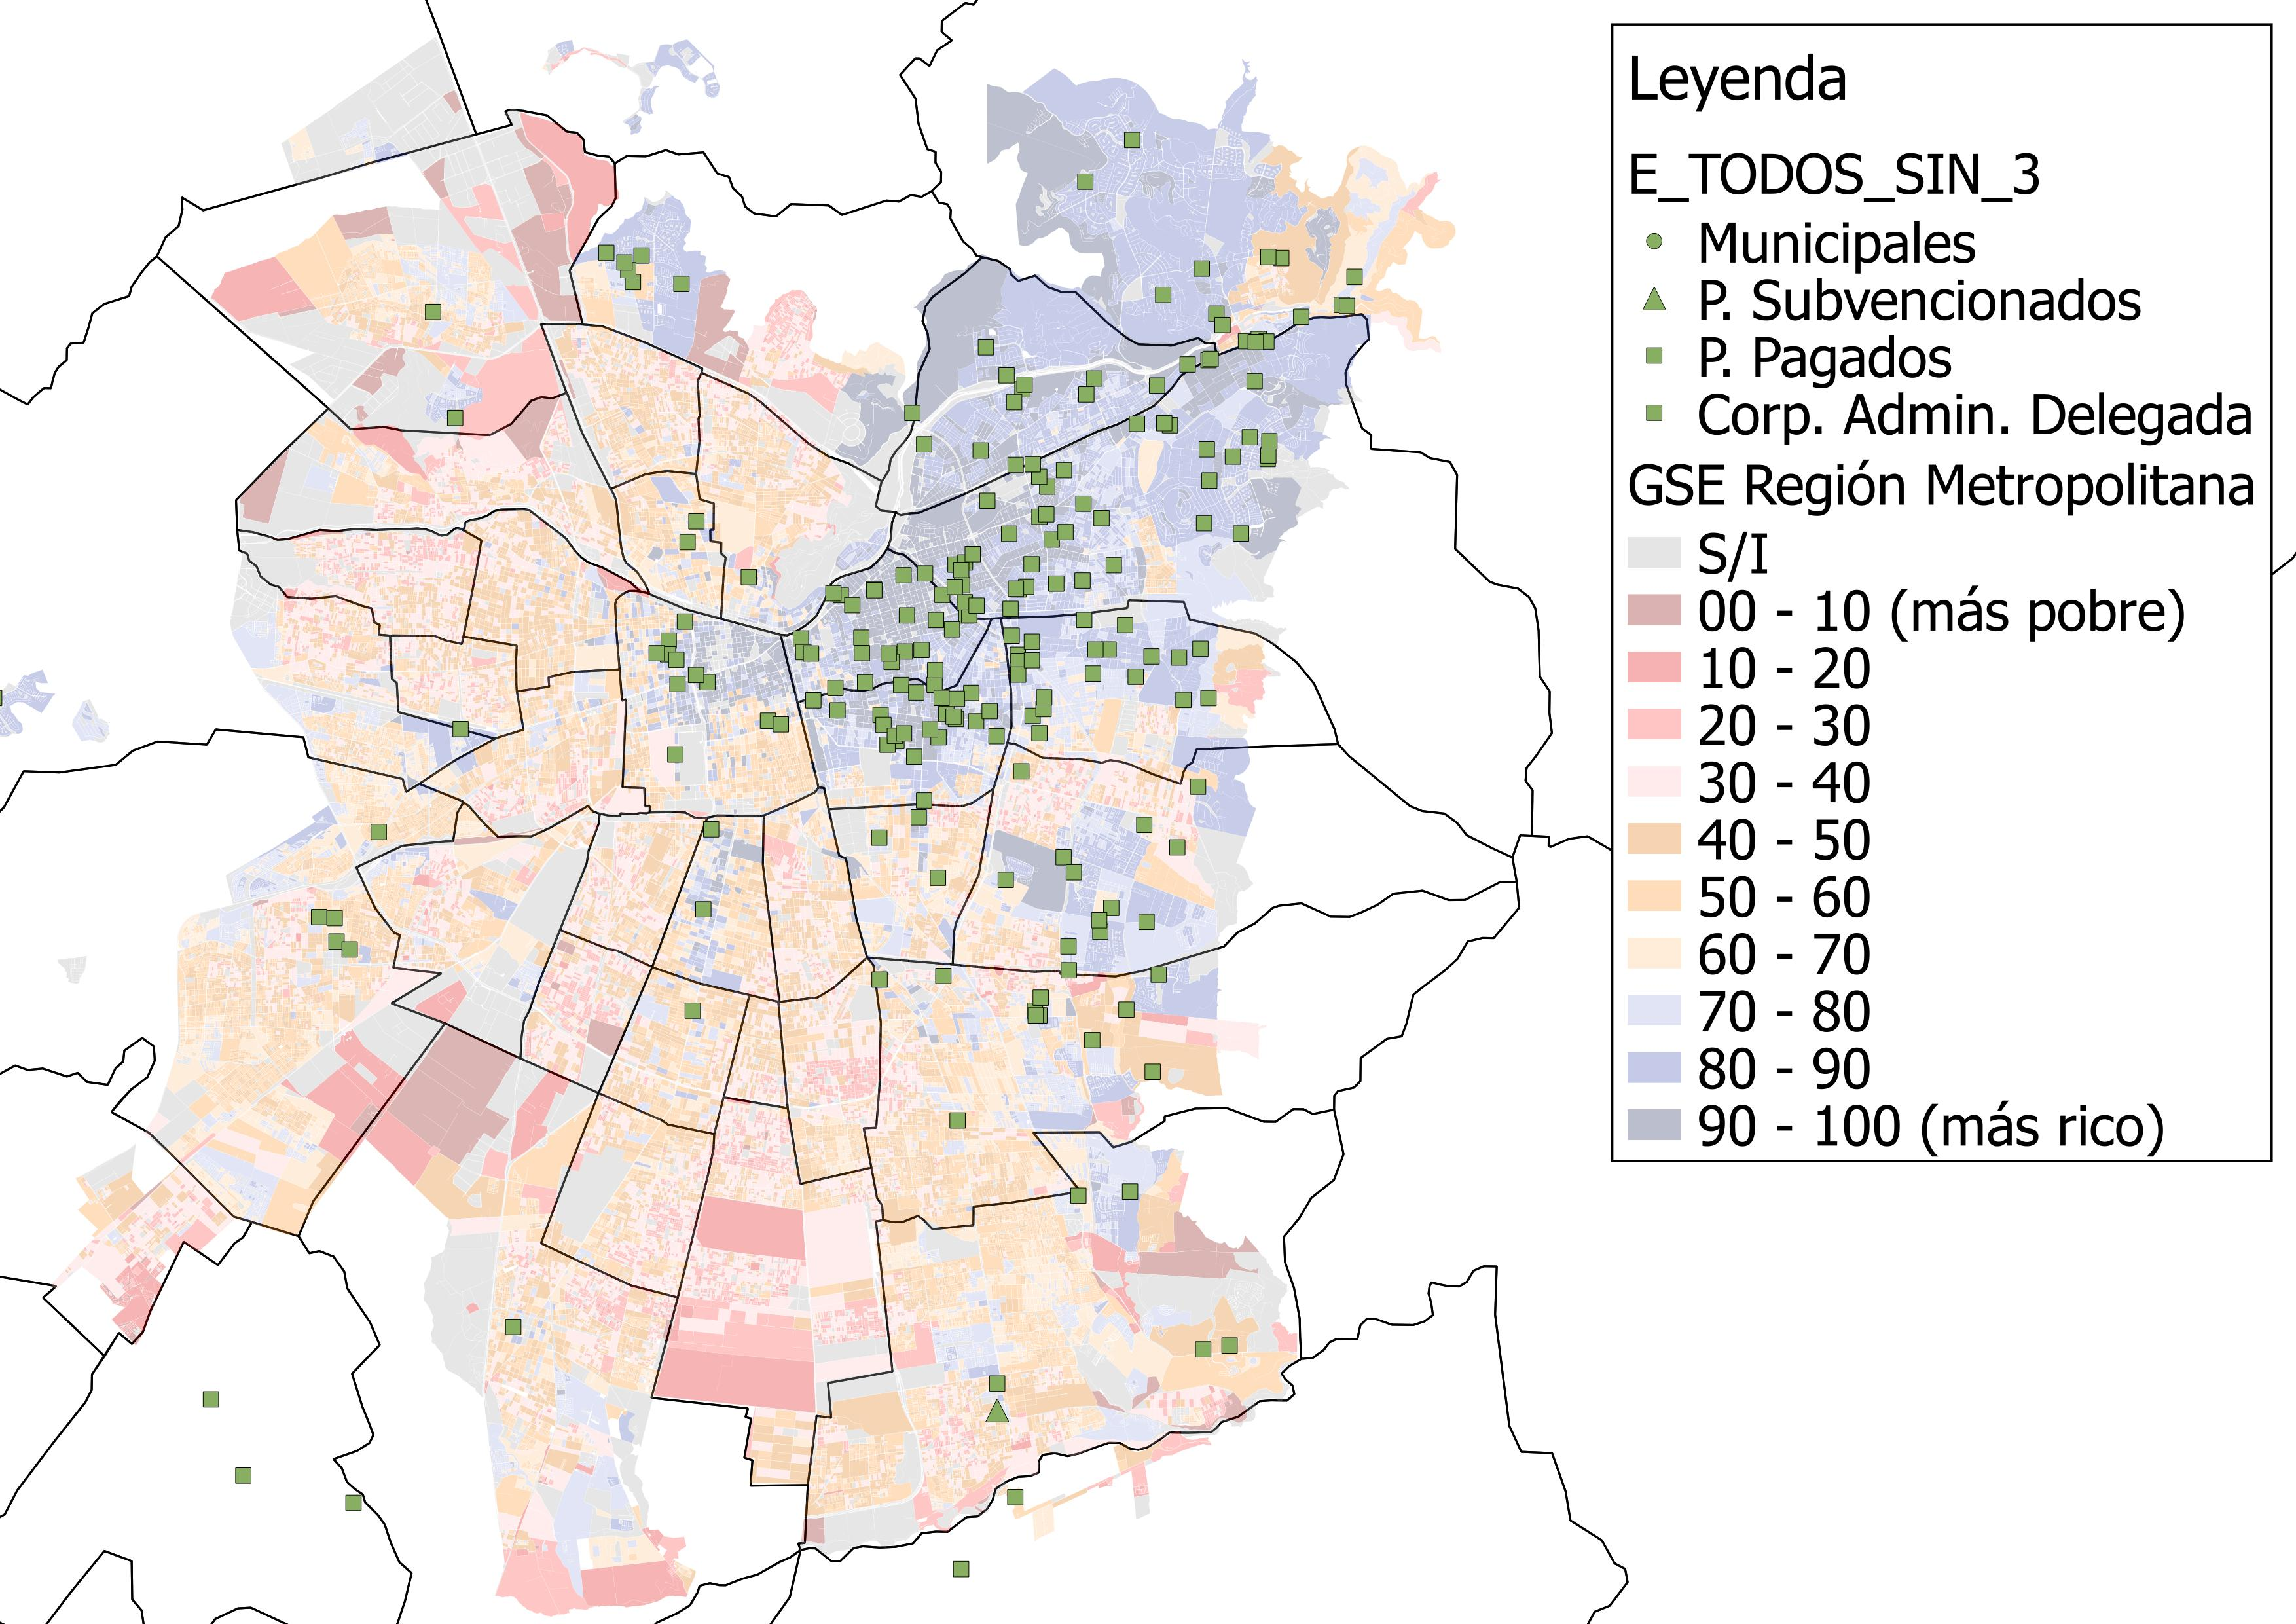
\includegraphics[width=7.5cm]{images/establecimientos/E_TODOS_SIN_3.jpg}}
 \caption{Mapas de clústers de establecimientos sobre mapa GSE de la Región Metropolitana.}
 \label{f:}
\end{figure}

\begin{figure}[h]
 \centering
  \subfloat[Establecimientos clúster E\_TODOS\_CON\_0.]{
   \label{f:}
    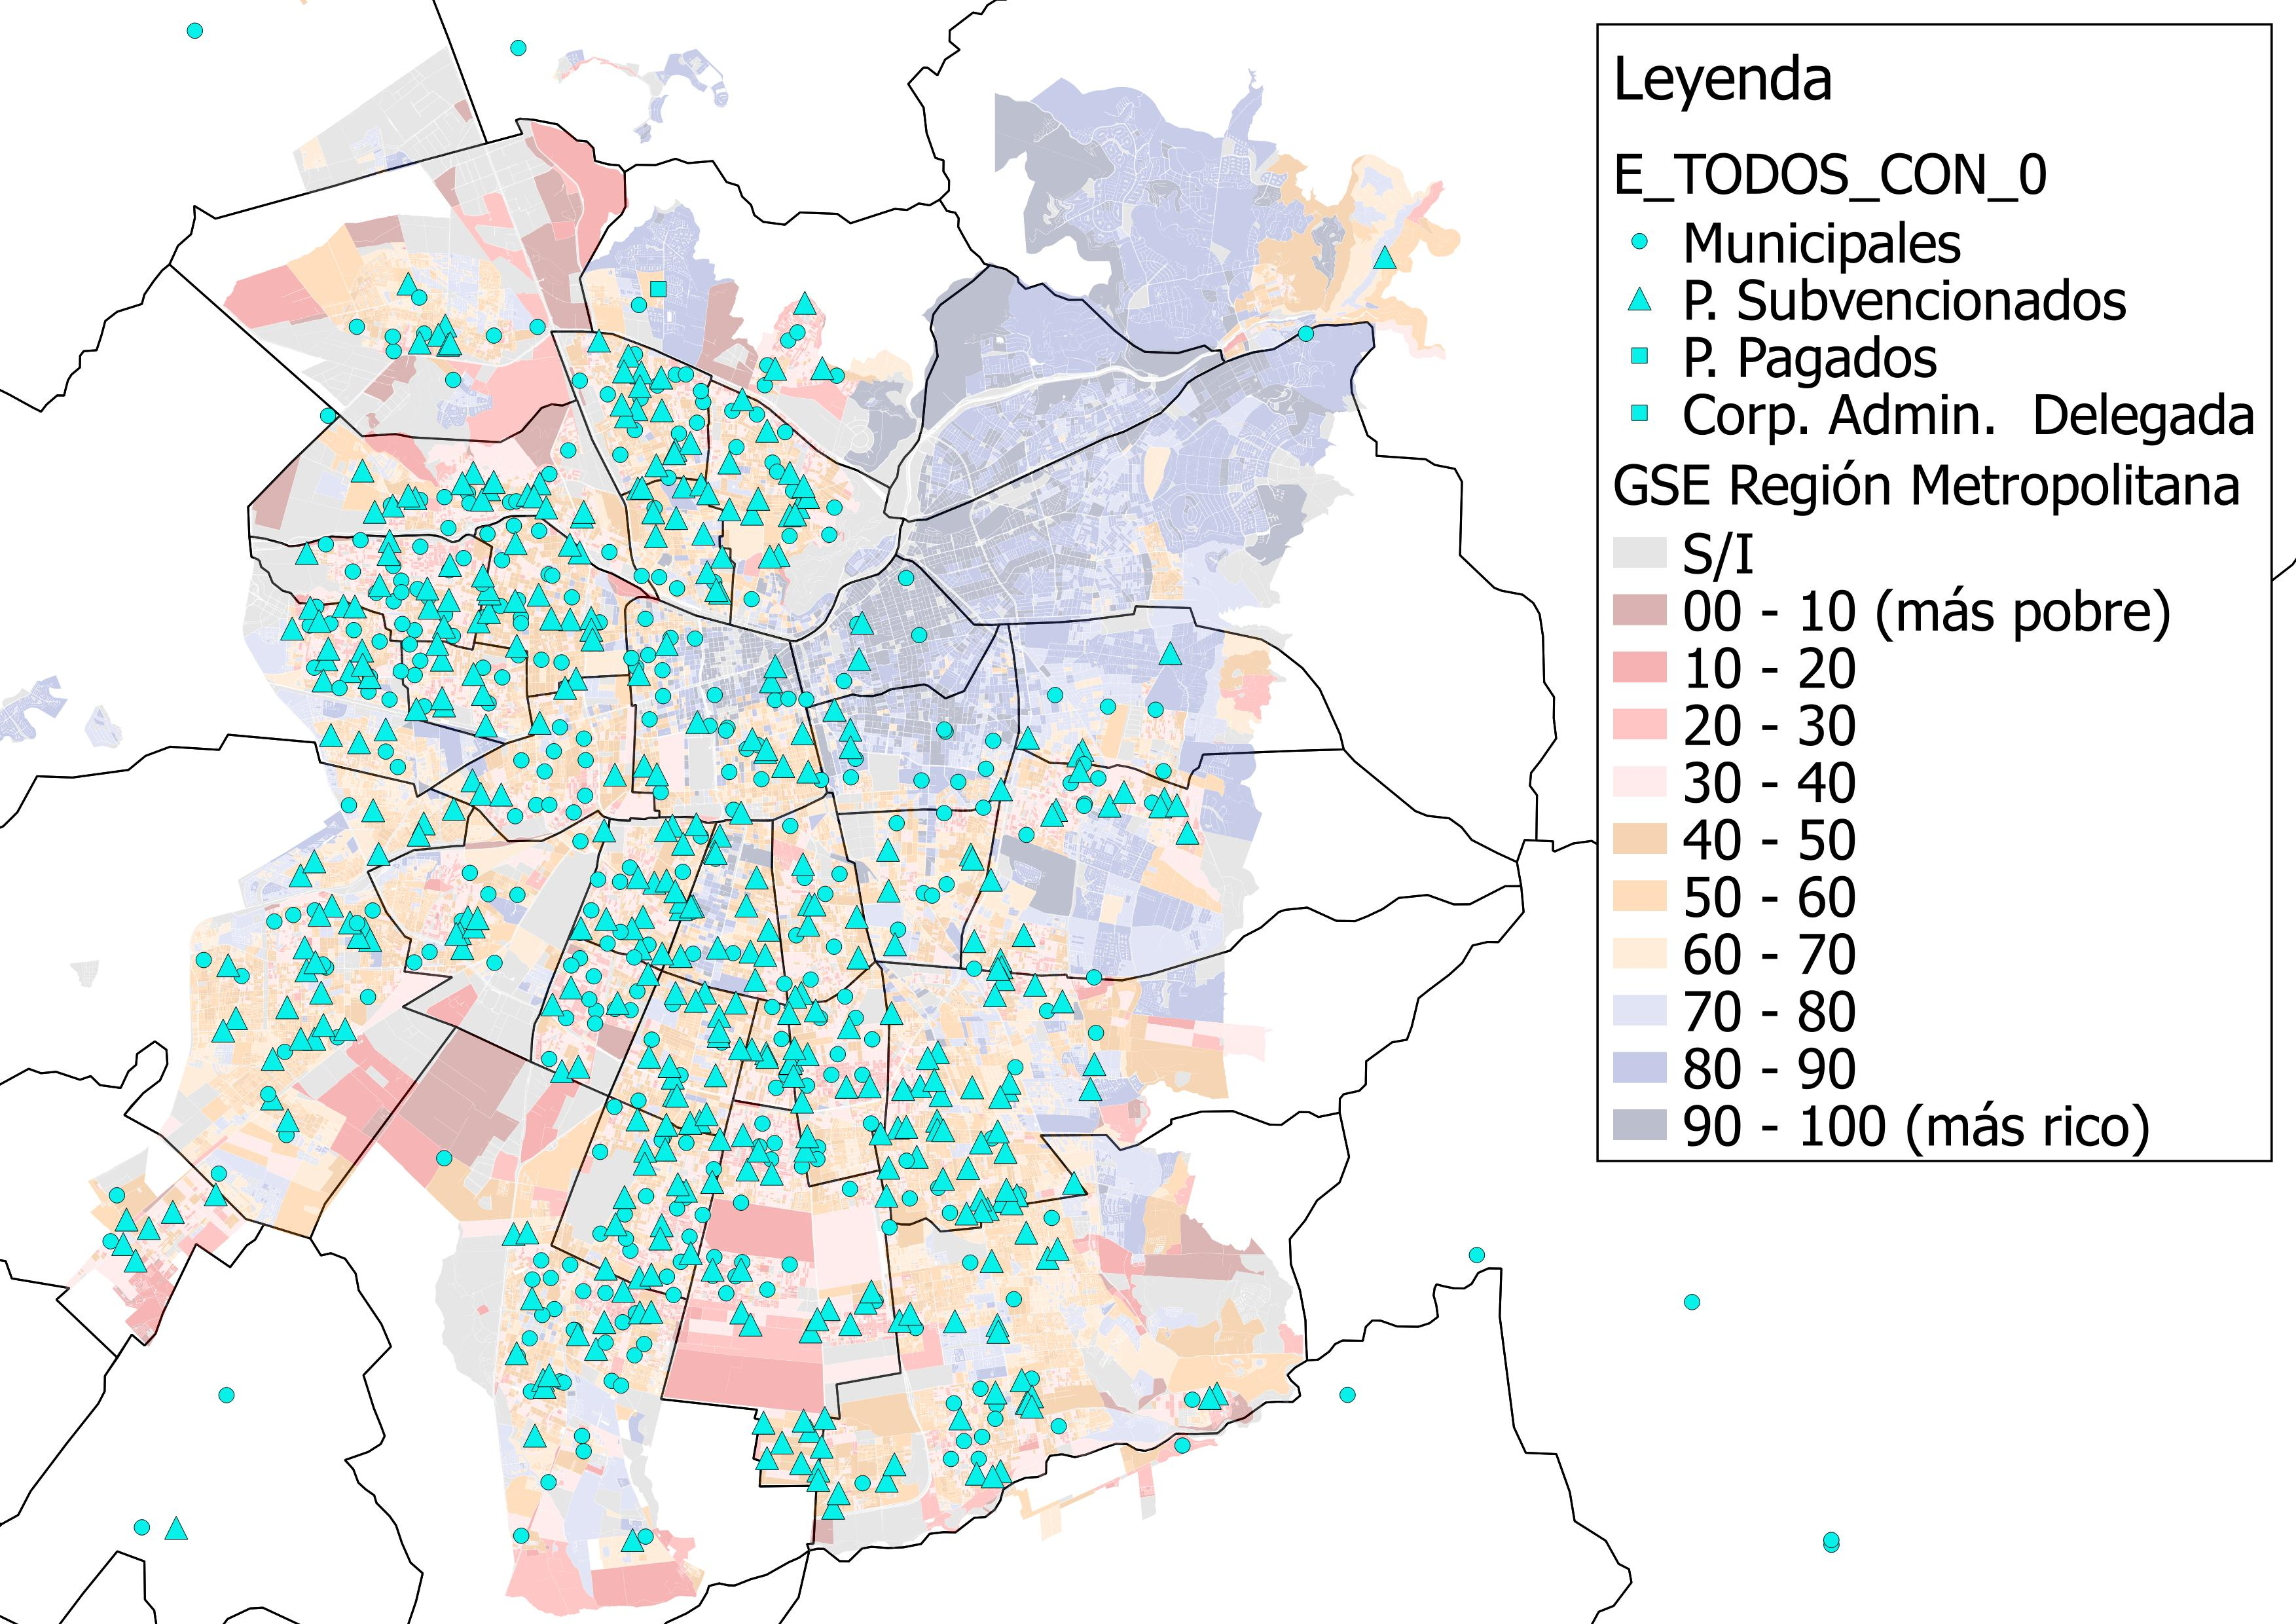
\includegraphics[width=7.5cm]{images/establecimientos/E_TODOS_CON_0.jpg}}
  \subfloat[Establecimientos clúster E\_TODOS\_CON\_1.]{
   \label{f:}
    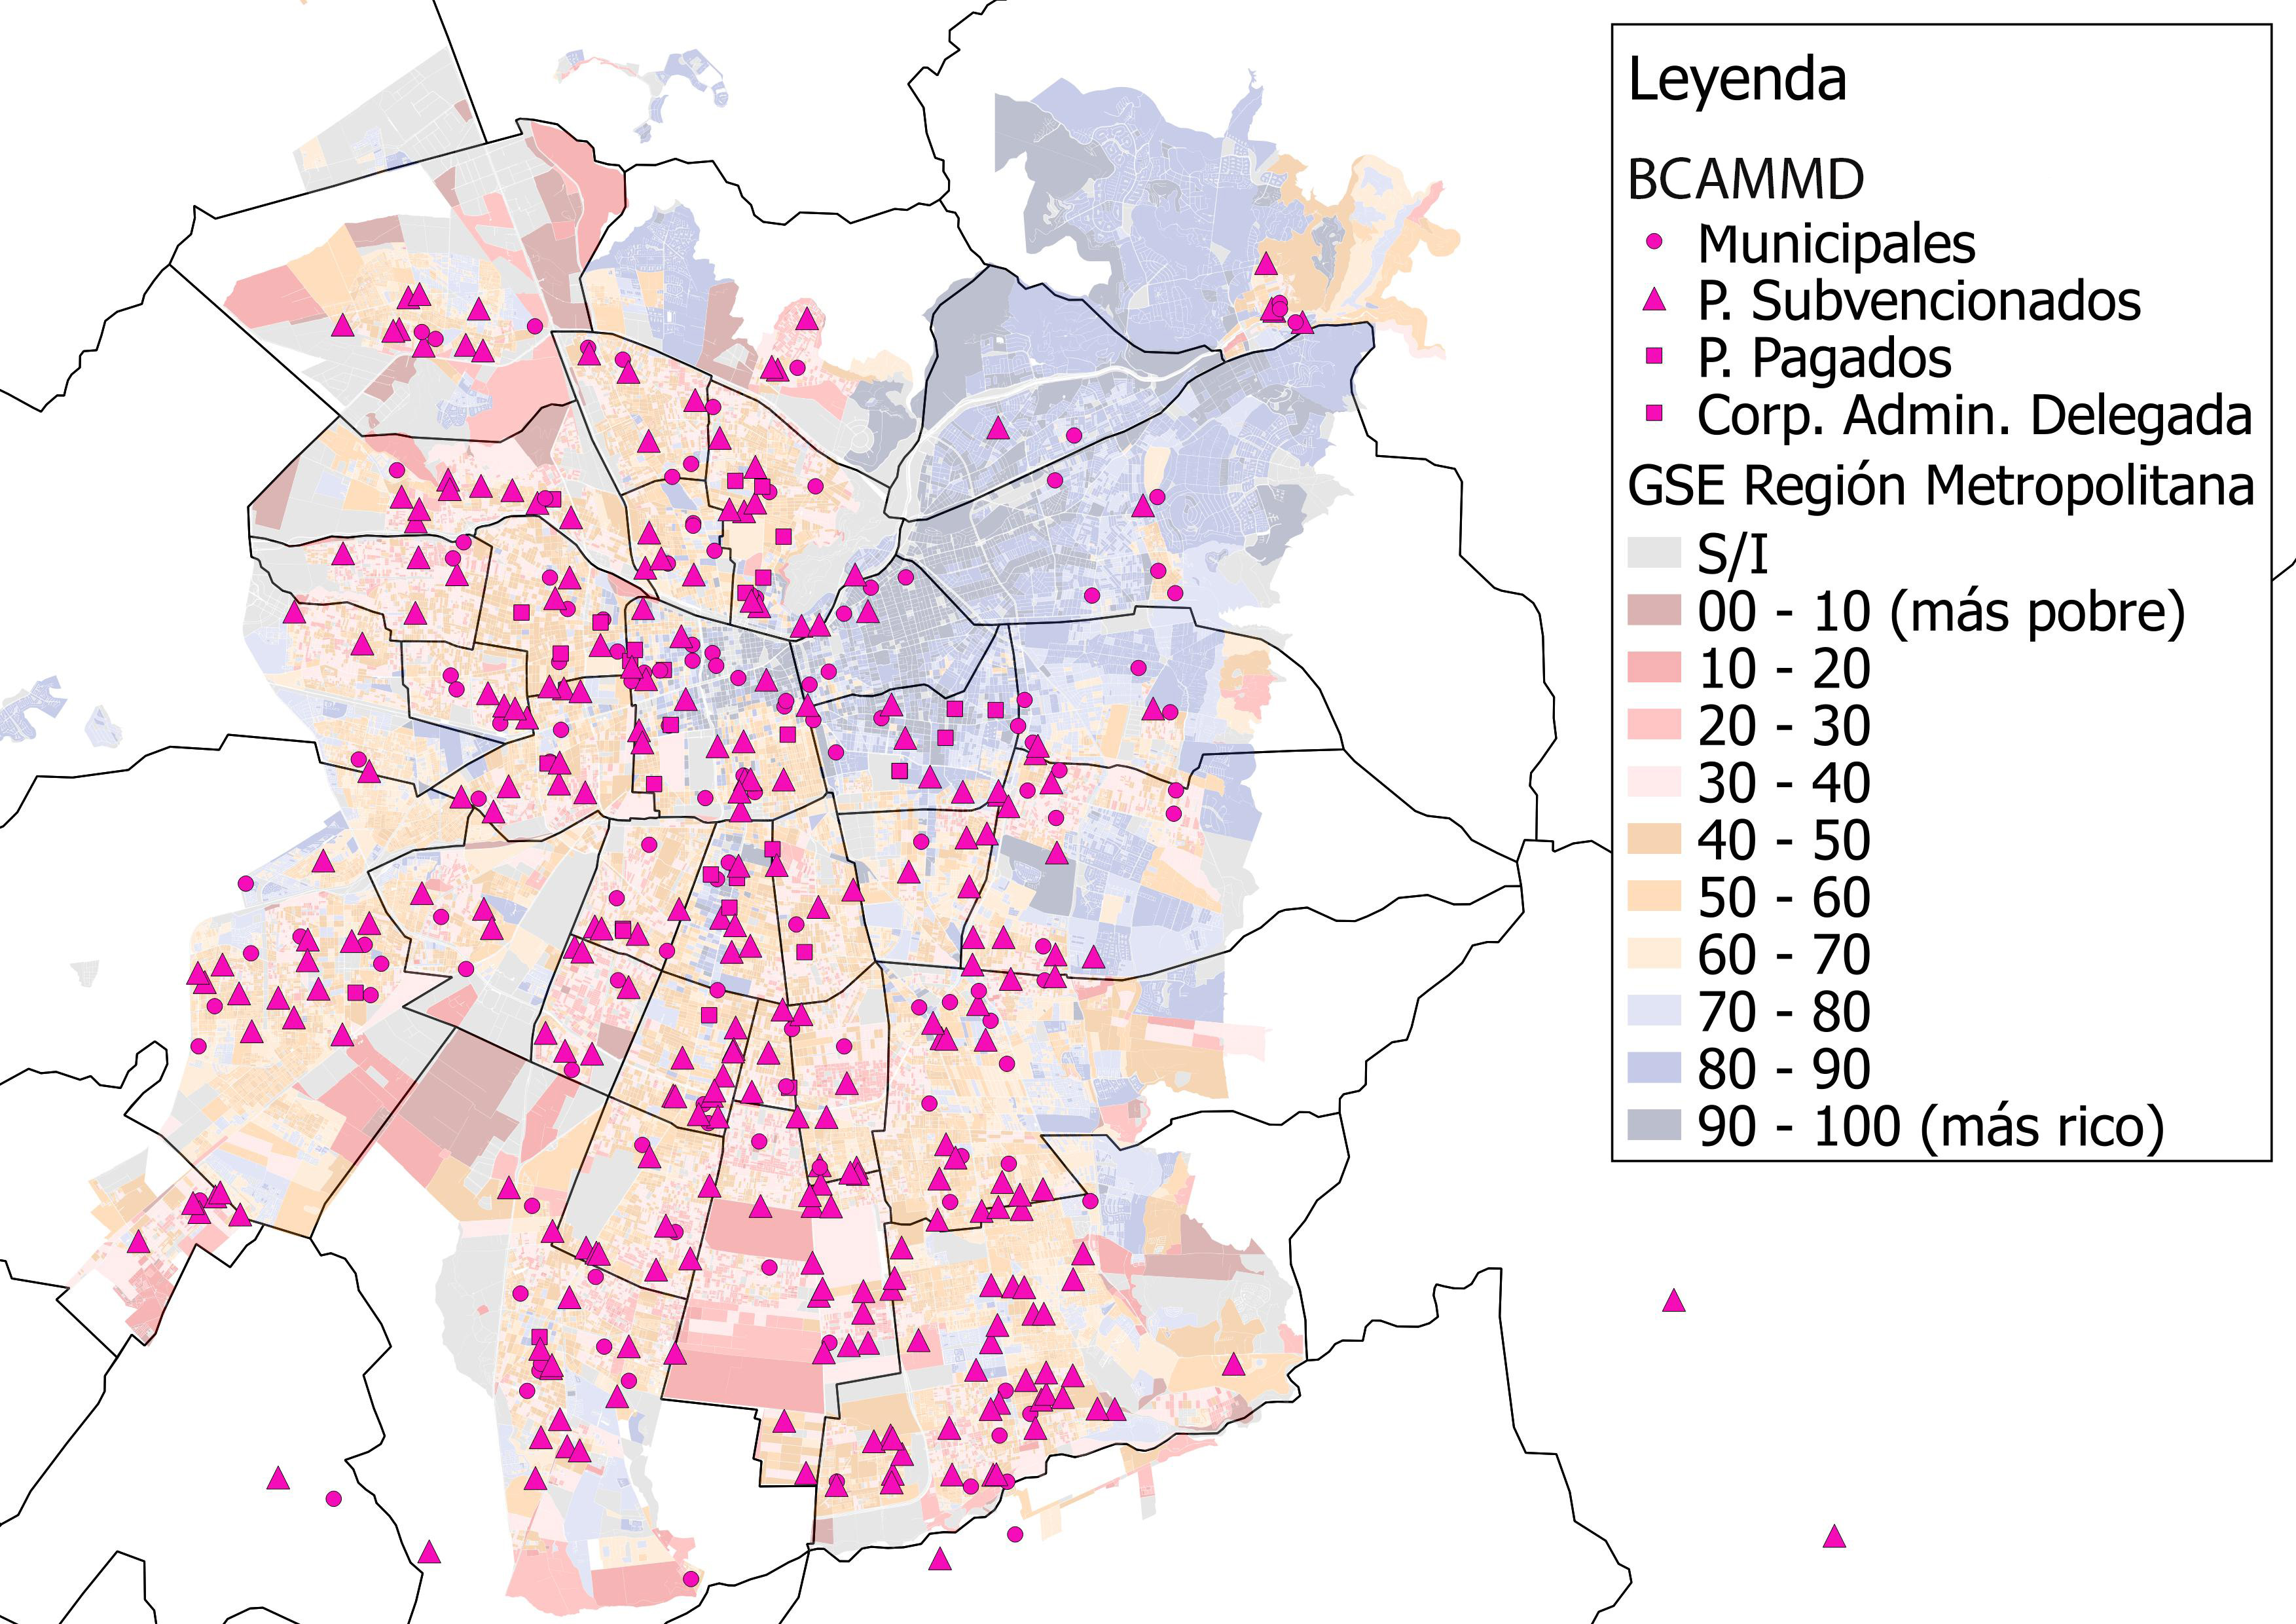
\includegraphics[width=7.5cm]{images/establecimientos/E_TODOS_CON_1.jpg}}\hspace{1mm}
  \subfloat[Establecimientos clúster E\_TODOS\_CON\_2.]{
   \label{f:}
    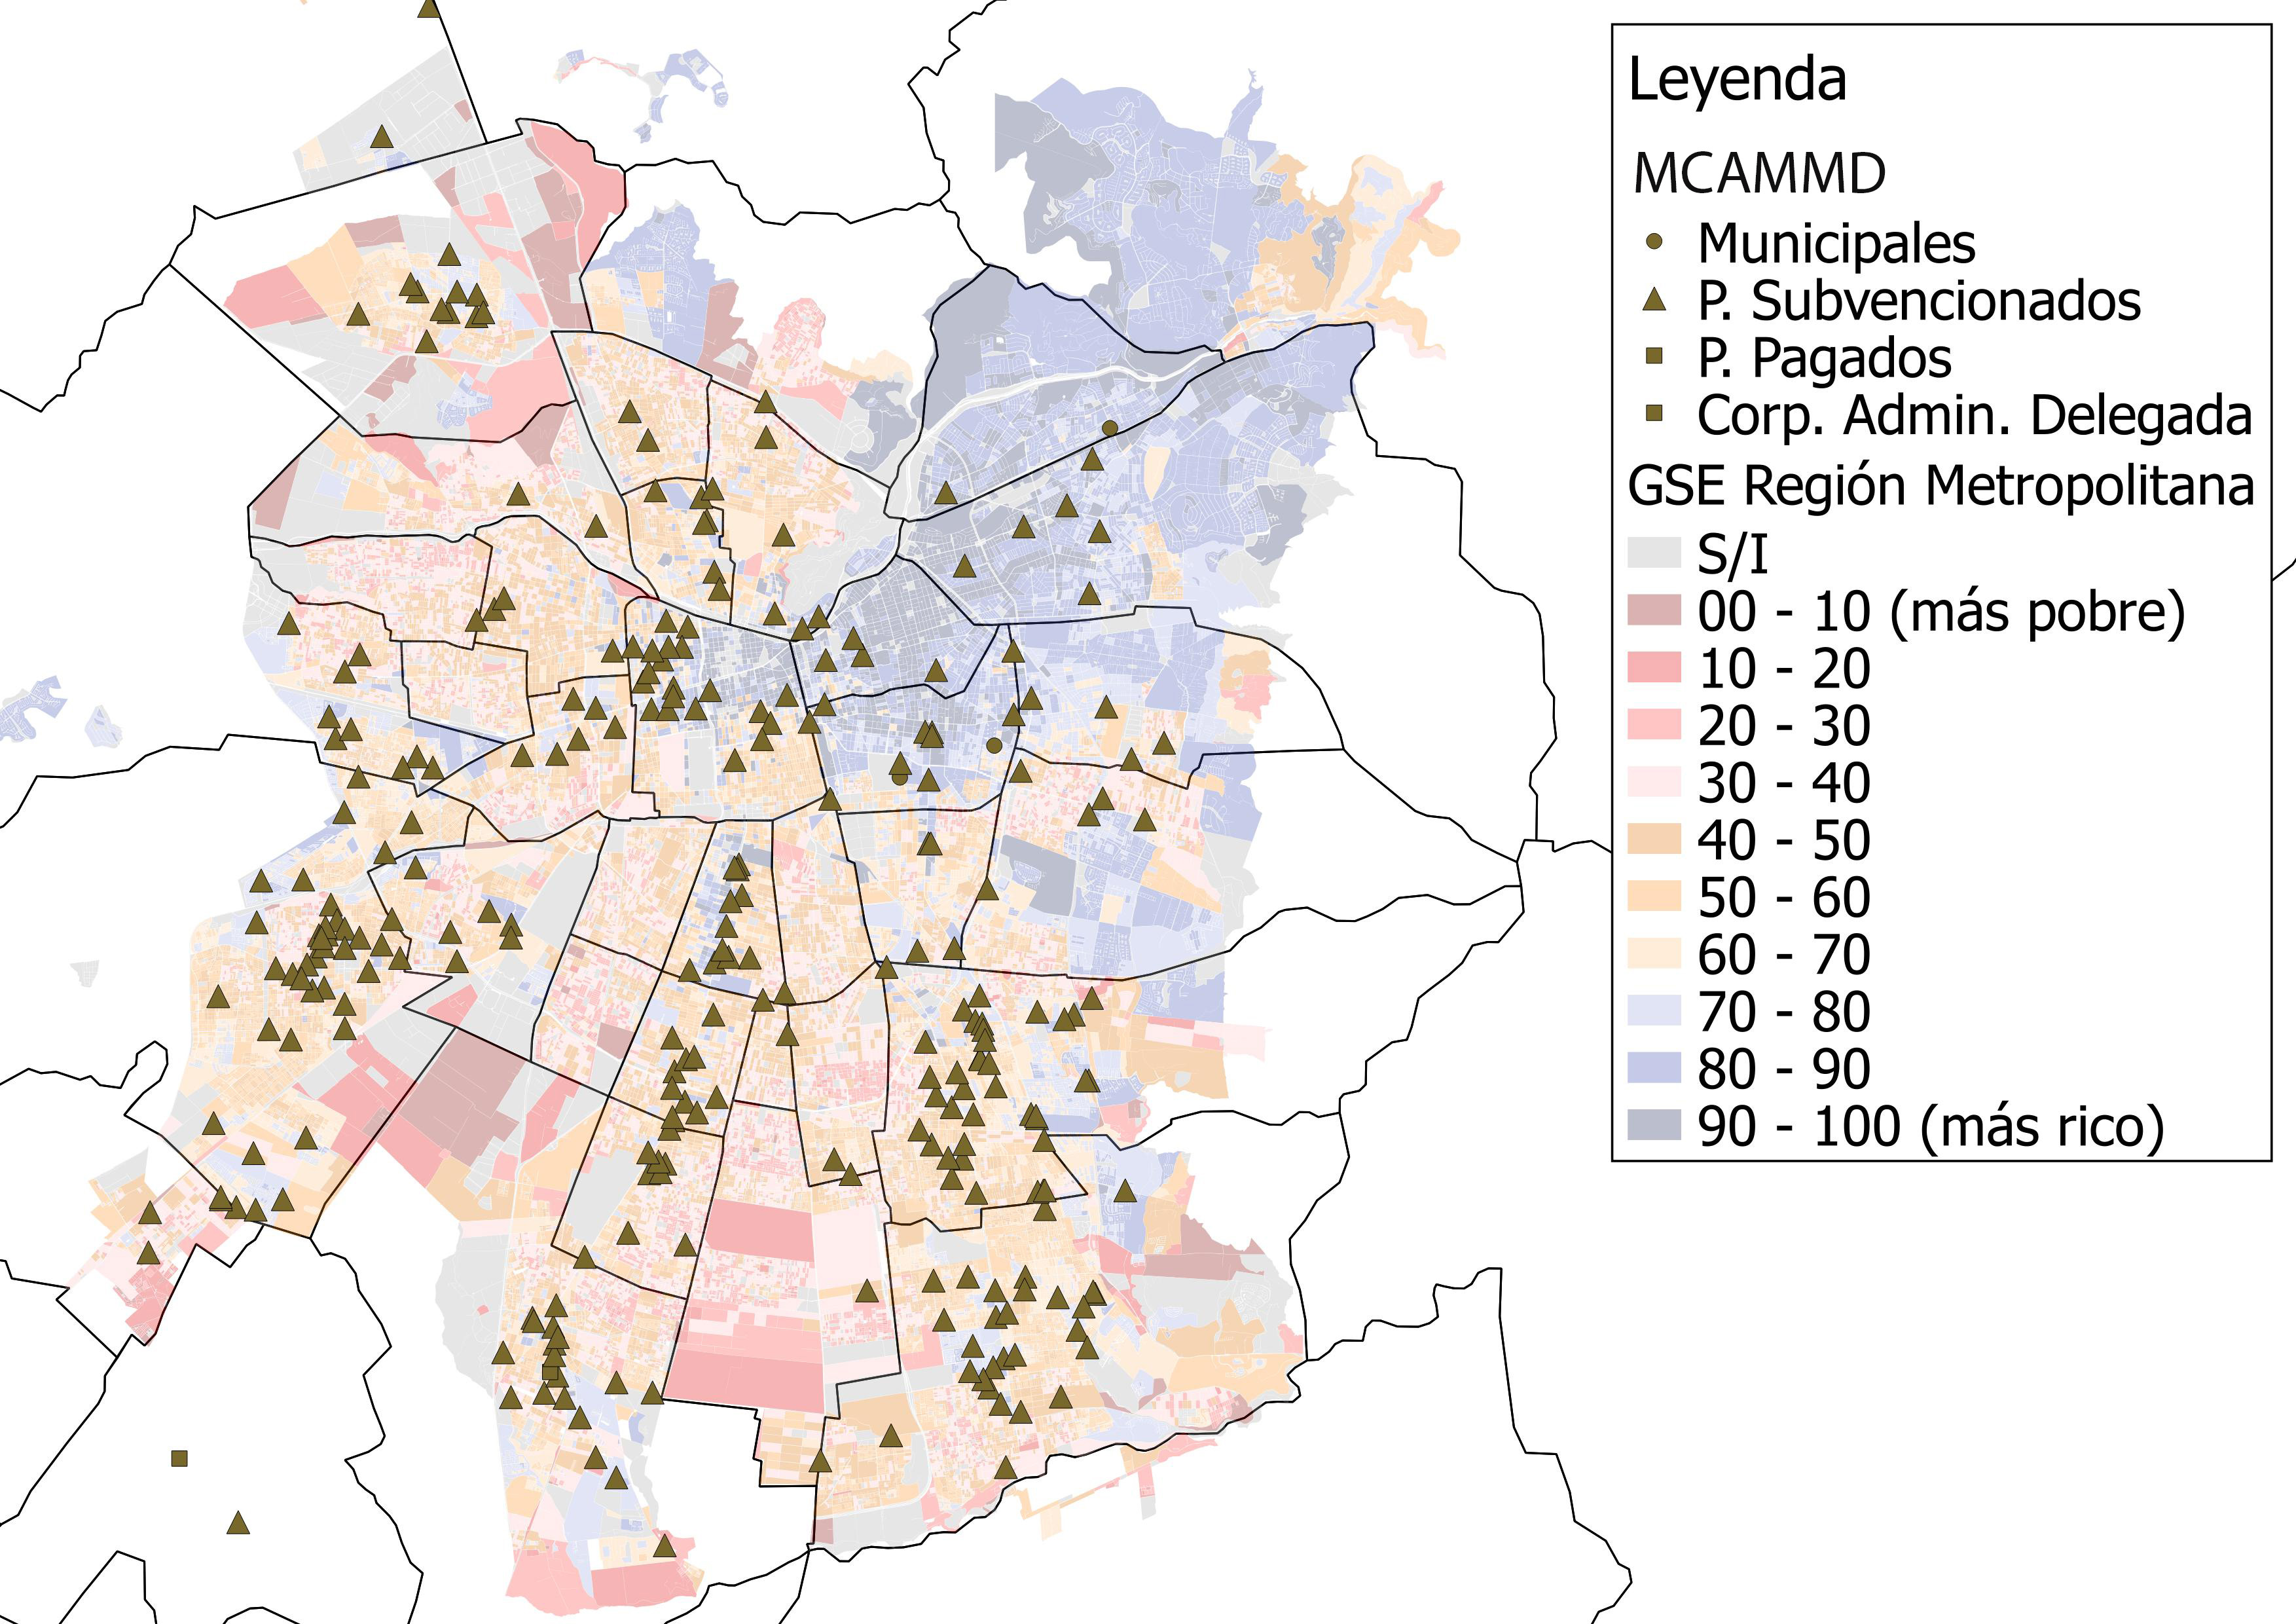
\includegraphics[width=7.5cm]{images/establecimientos/E_TODOS_CON_2.jpg}}
  \subfloat[Establecimientos clúster E\_TODOS\_CON\_3.]{
   \label{f:}
    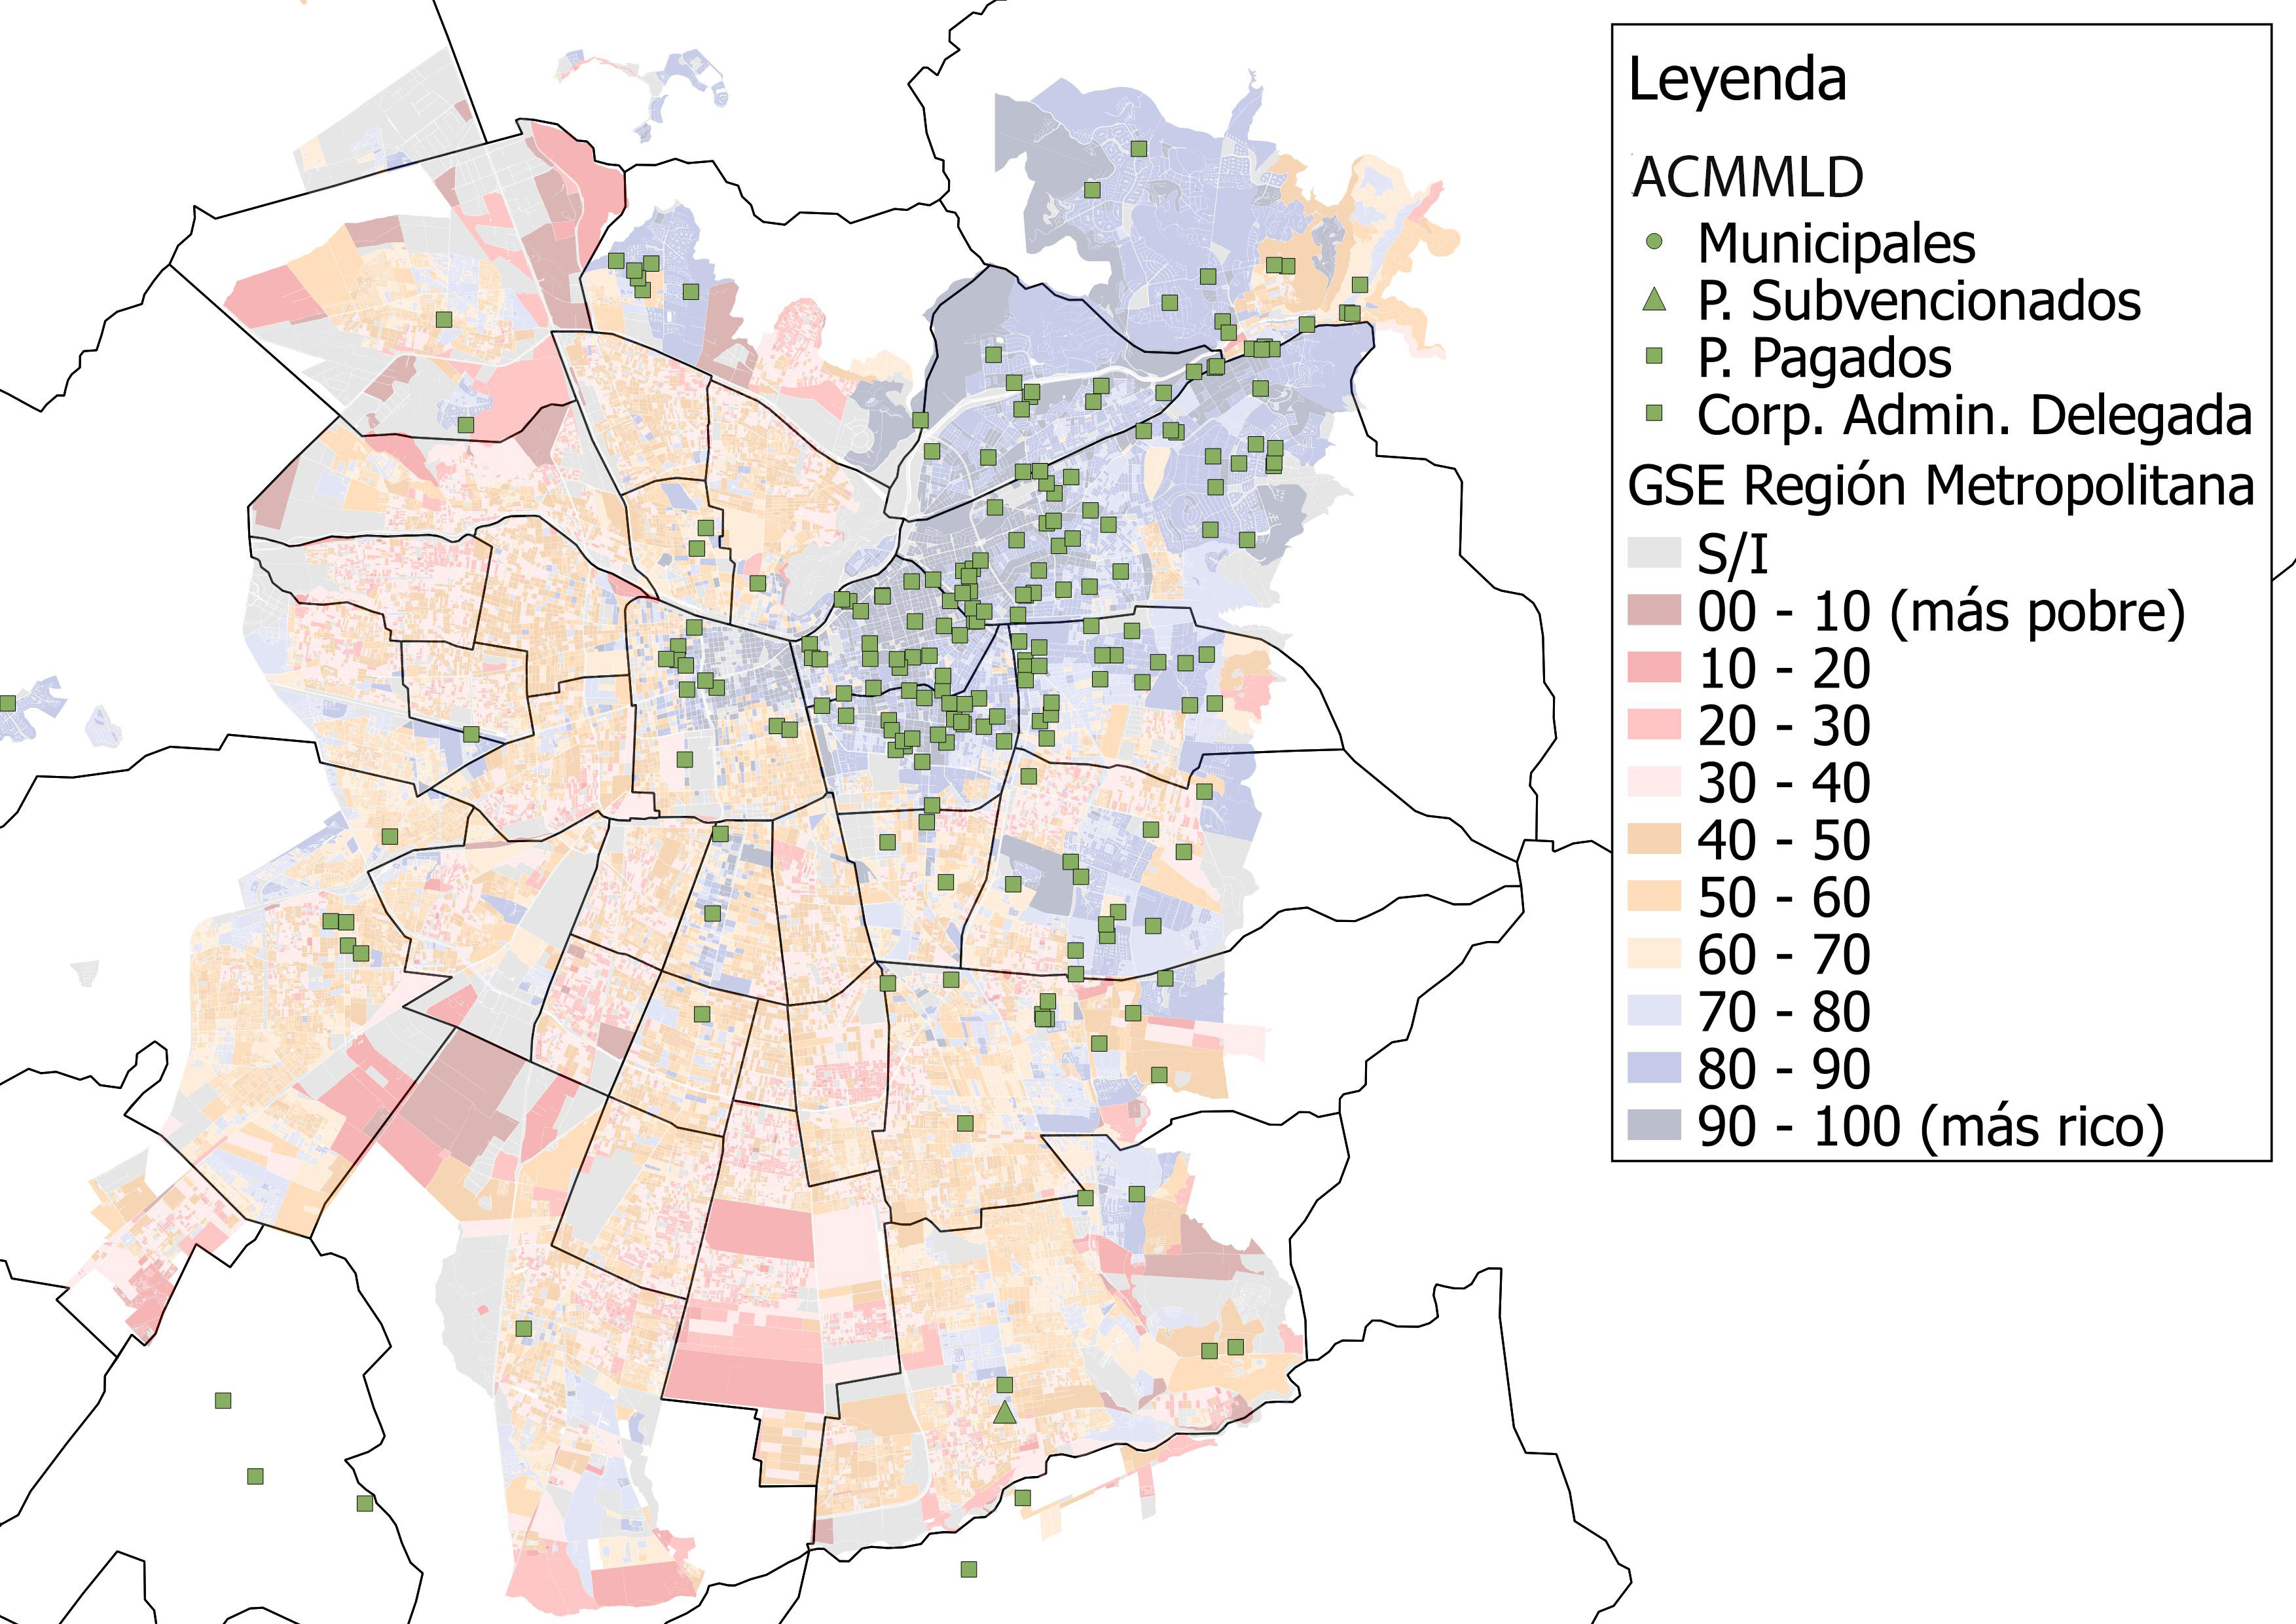
\includegraphics[width=7.5cm]{images/establecimientos/E_TODOS_CON_3.jpg}}
 \caption{Mapas de clústers de establecimientos (con atributos relacionales) sobre mapa GSE de la Región Metropolitana.}
 \label{f:}
\end{figure}

\begin{figure}[h]
 \centering
  \subfloat[Matrículas en colegios de E\_TODOS\_SIN\_0.]{
   \label{f:}
    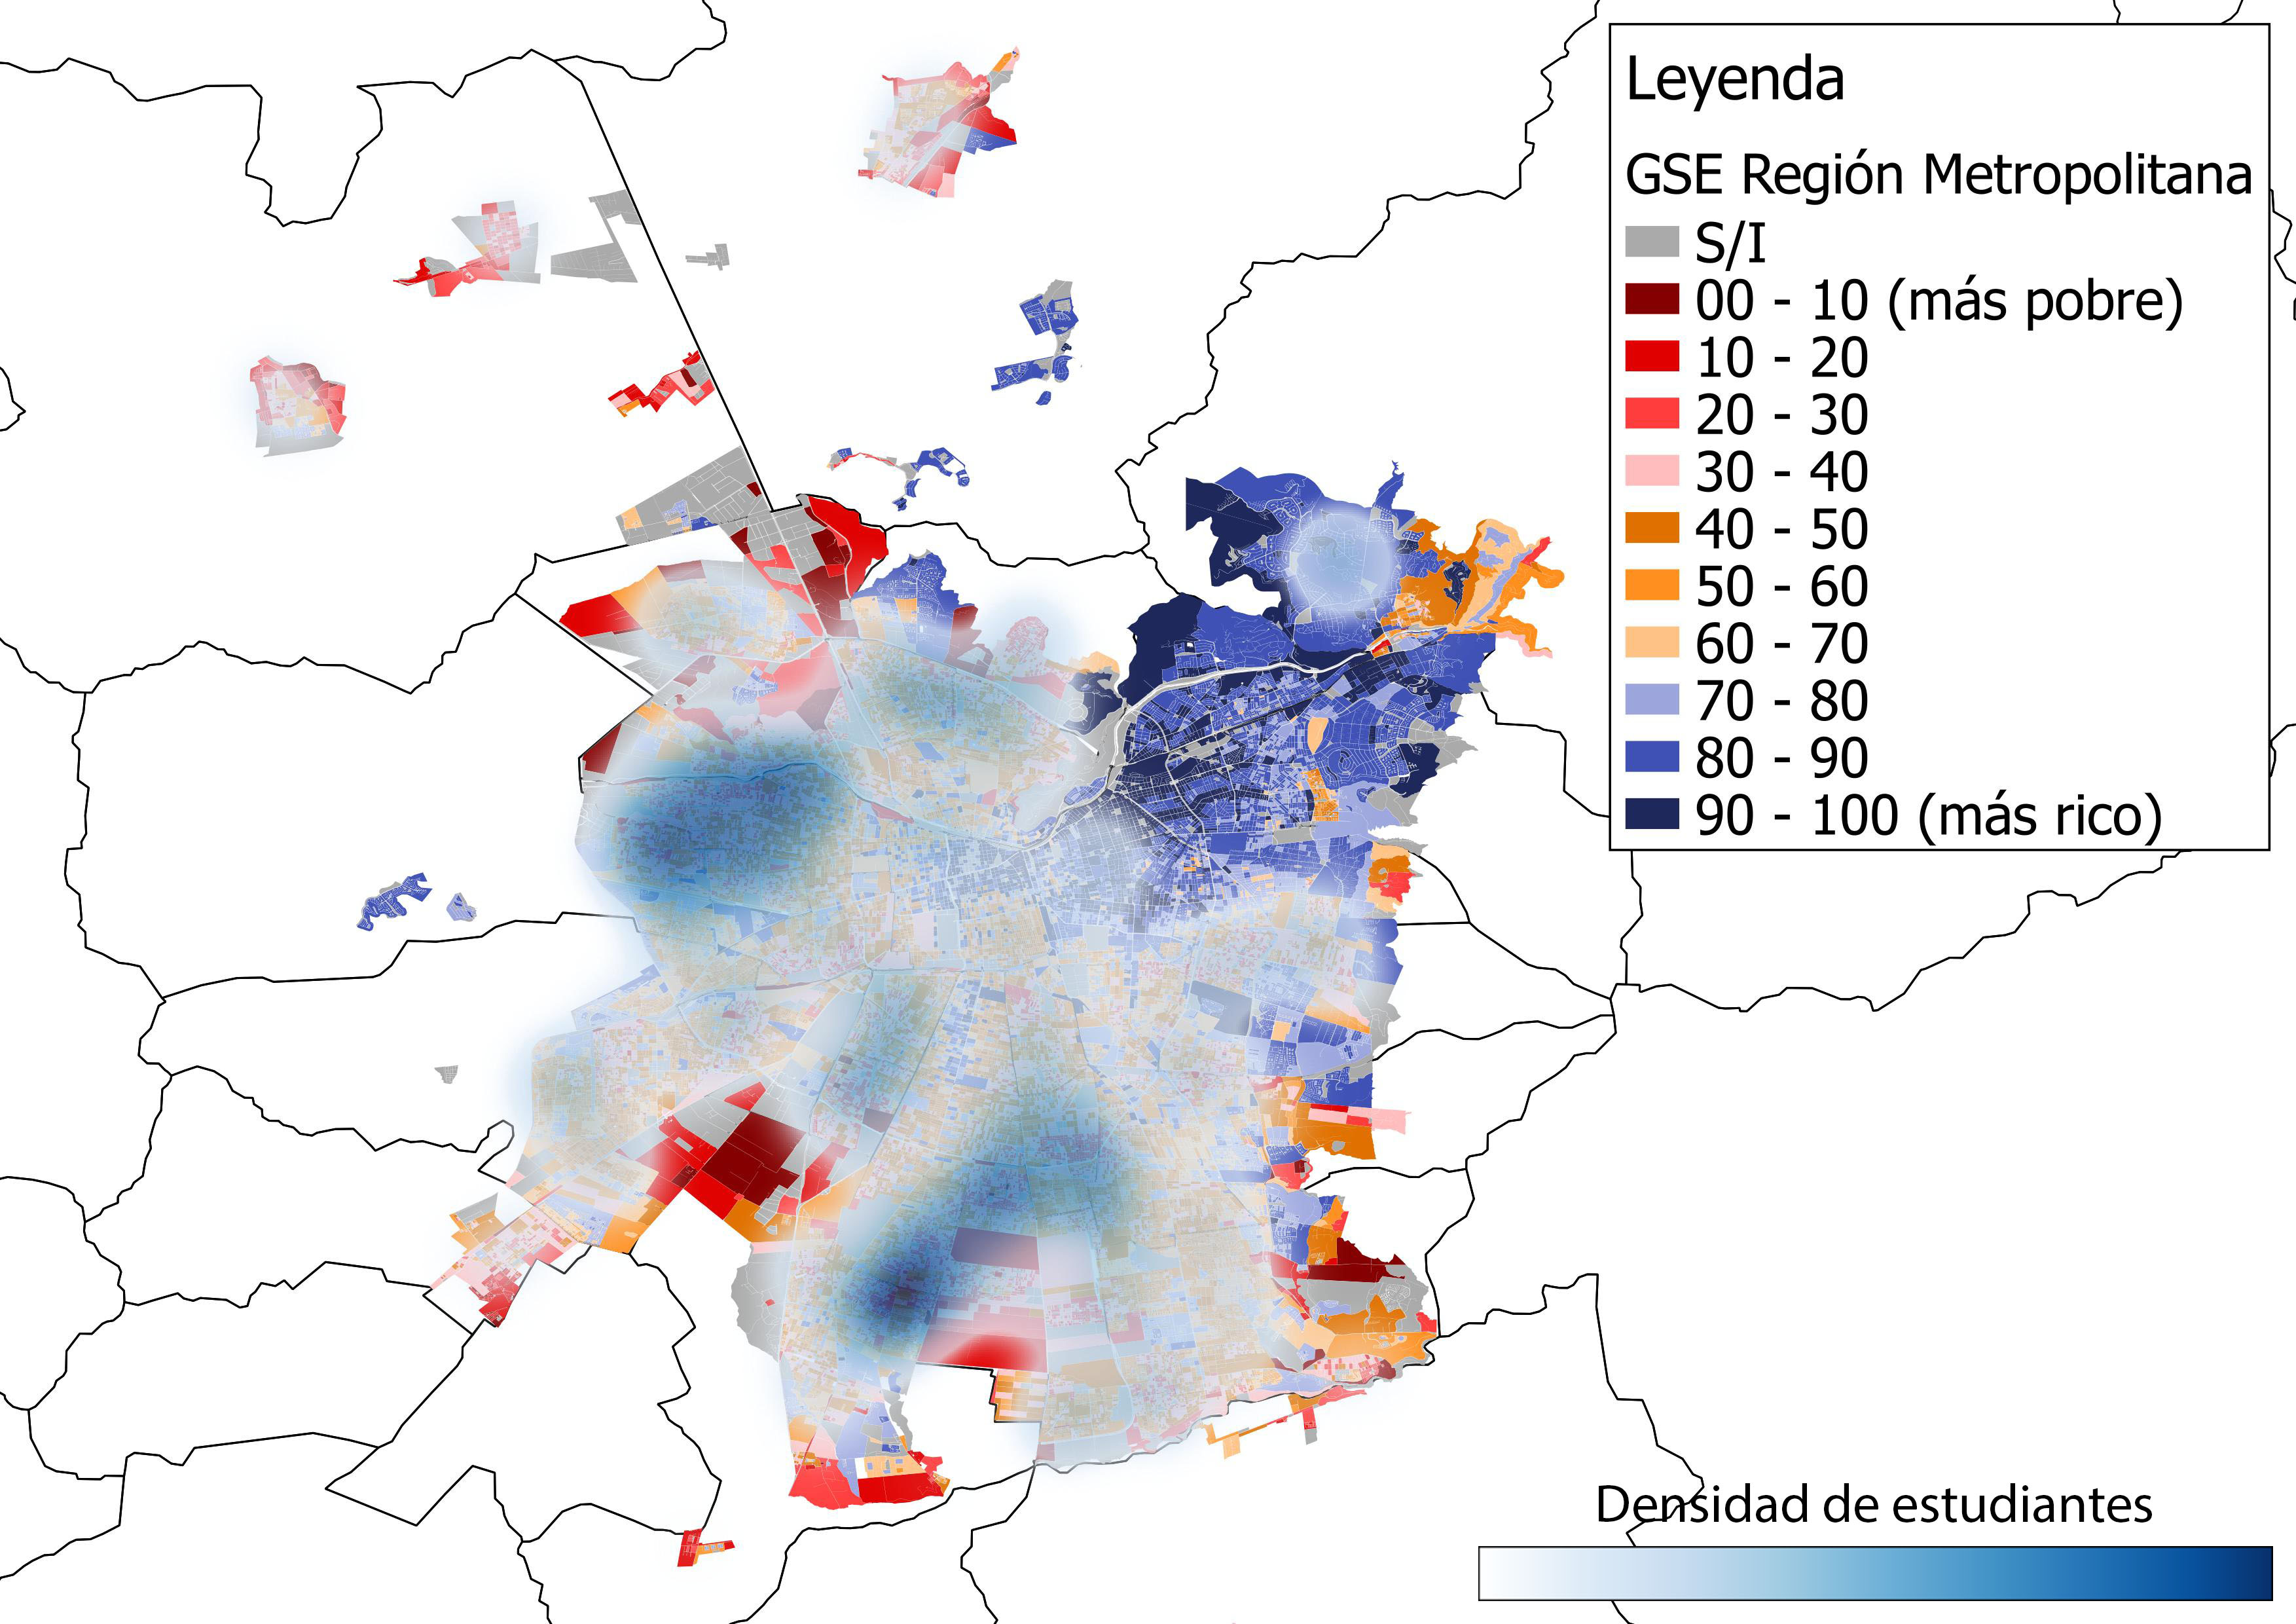
\includegraphics[width=7.5cm]{images/matriculas/E_SIN_0_final.jpg}}
  \subfloat[Matrículas en colegios de E\_TODOS\_SIN\_1.]{
   \label{f:}
    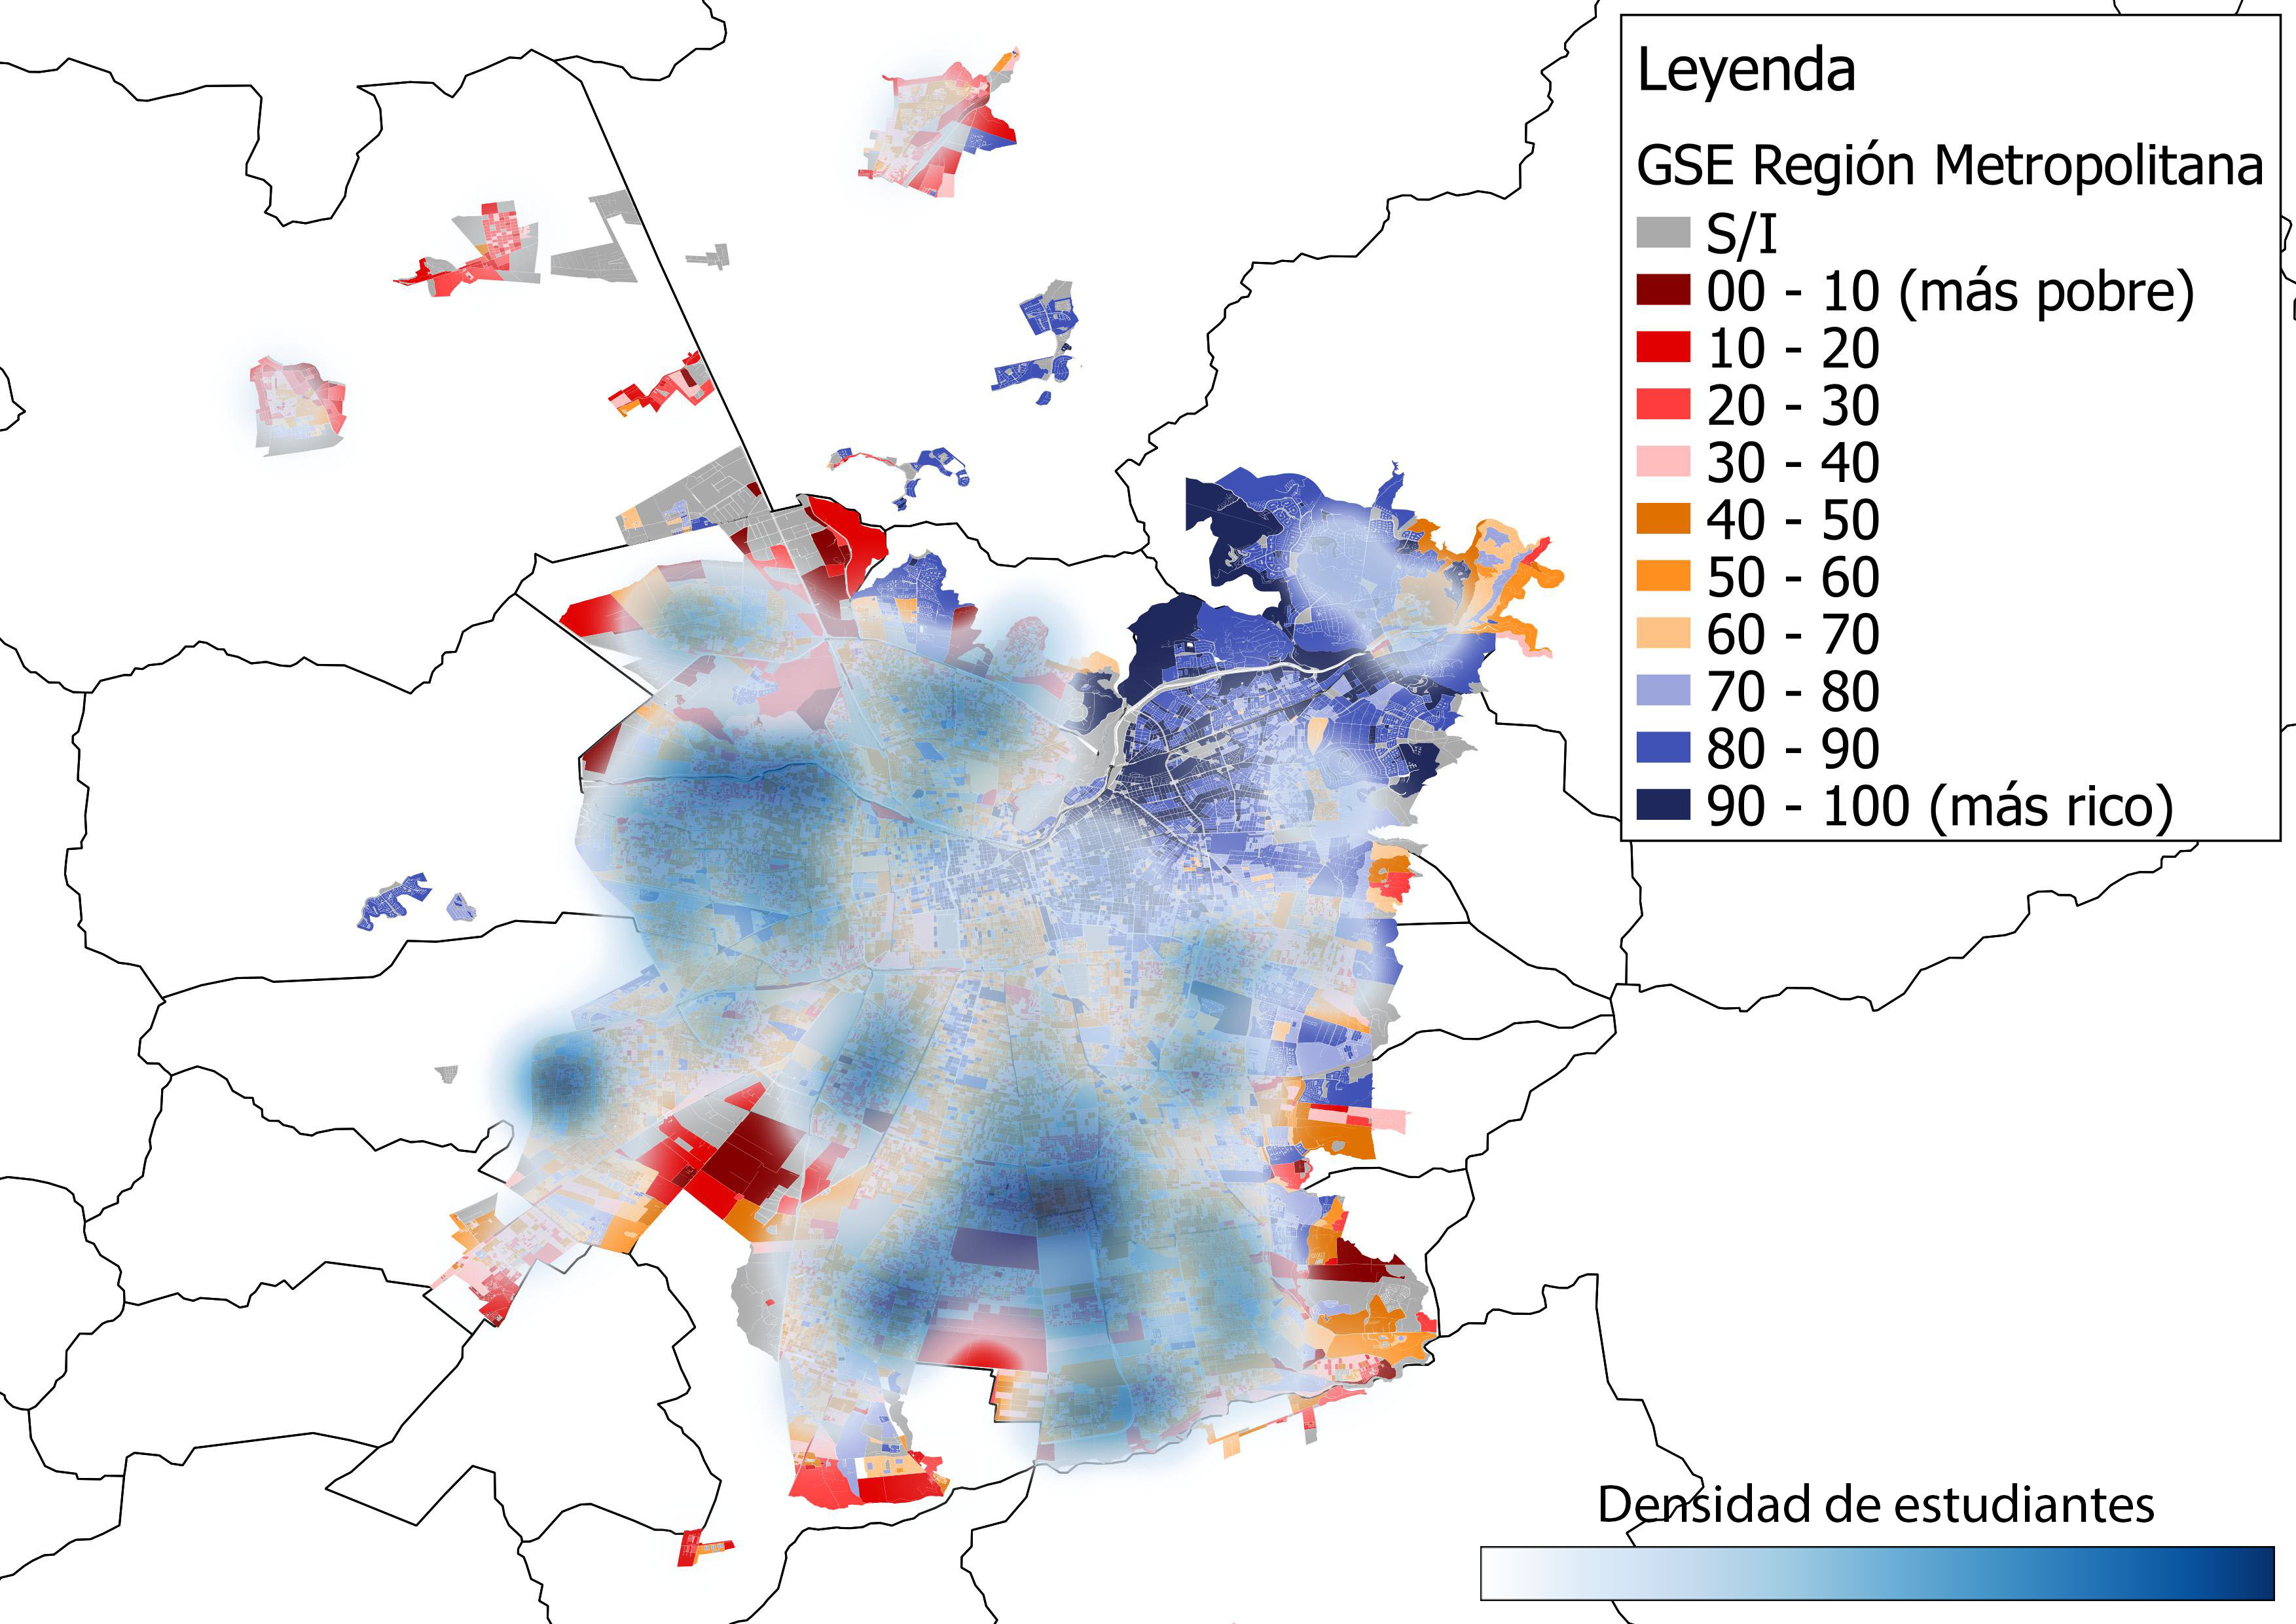
\includegraphics[width=7.5cm]{images/matriculas/E_SIN_1_final.jpg}}\hspace{1mm}
  \subfloat[Matrículas en colegios de E\_TODOS\_SIN\_2.]{
   \label{f:}
    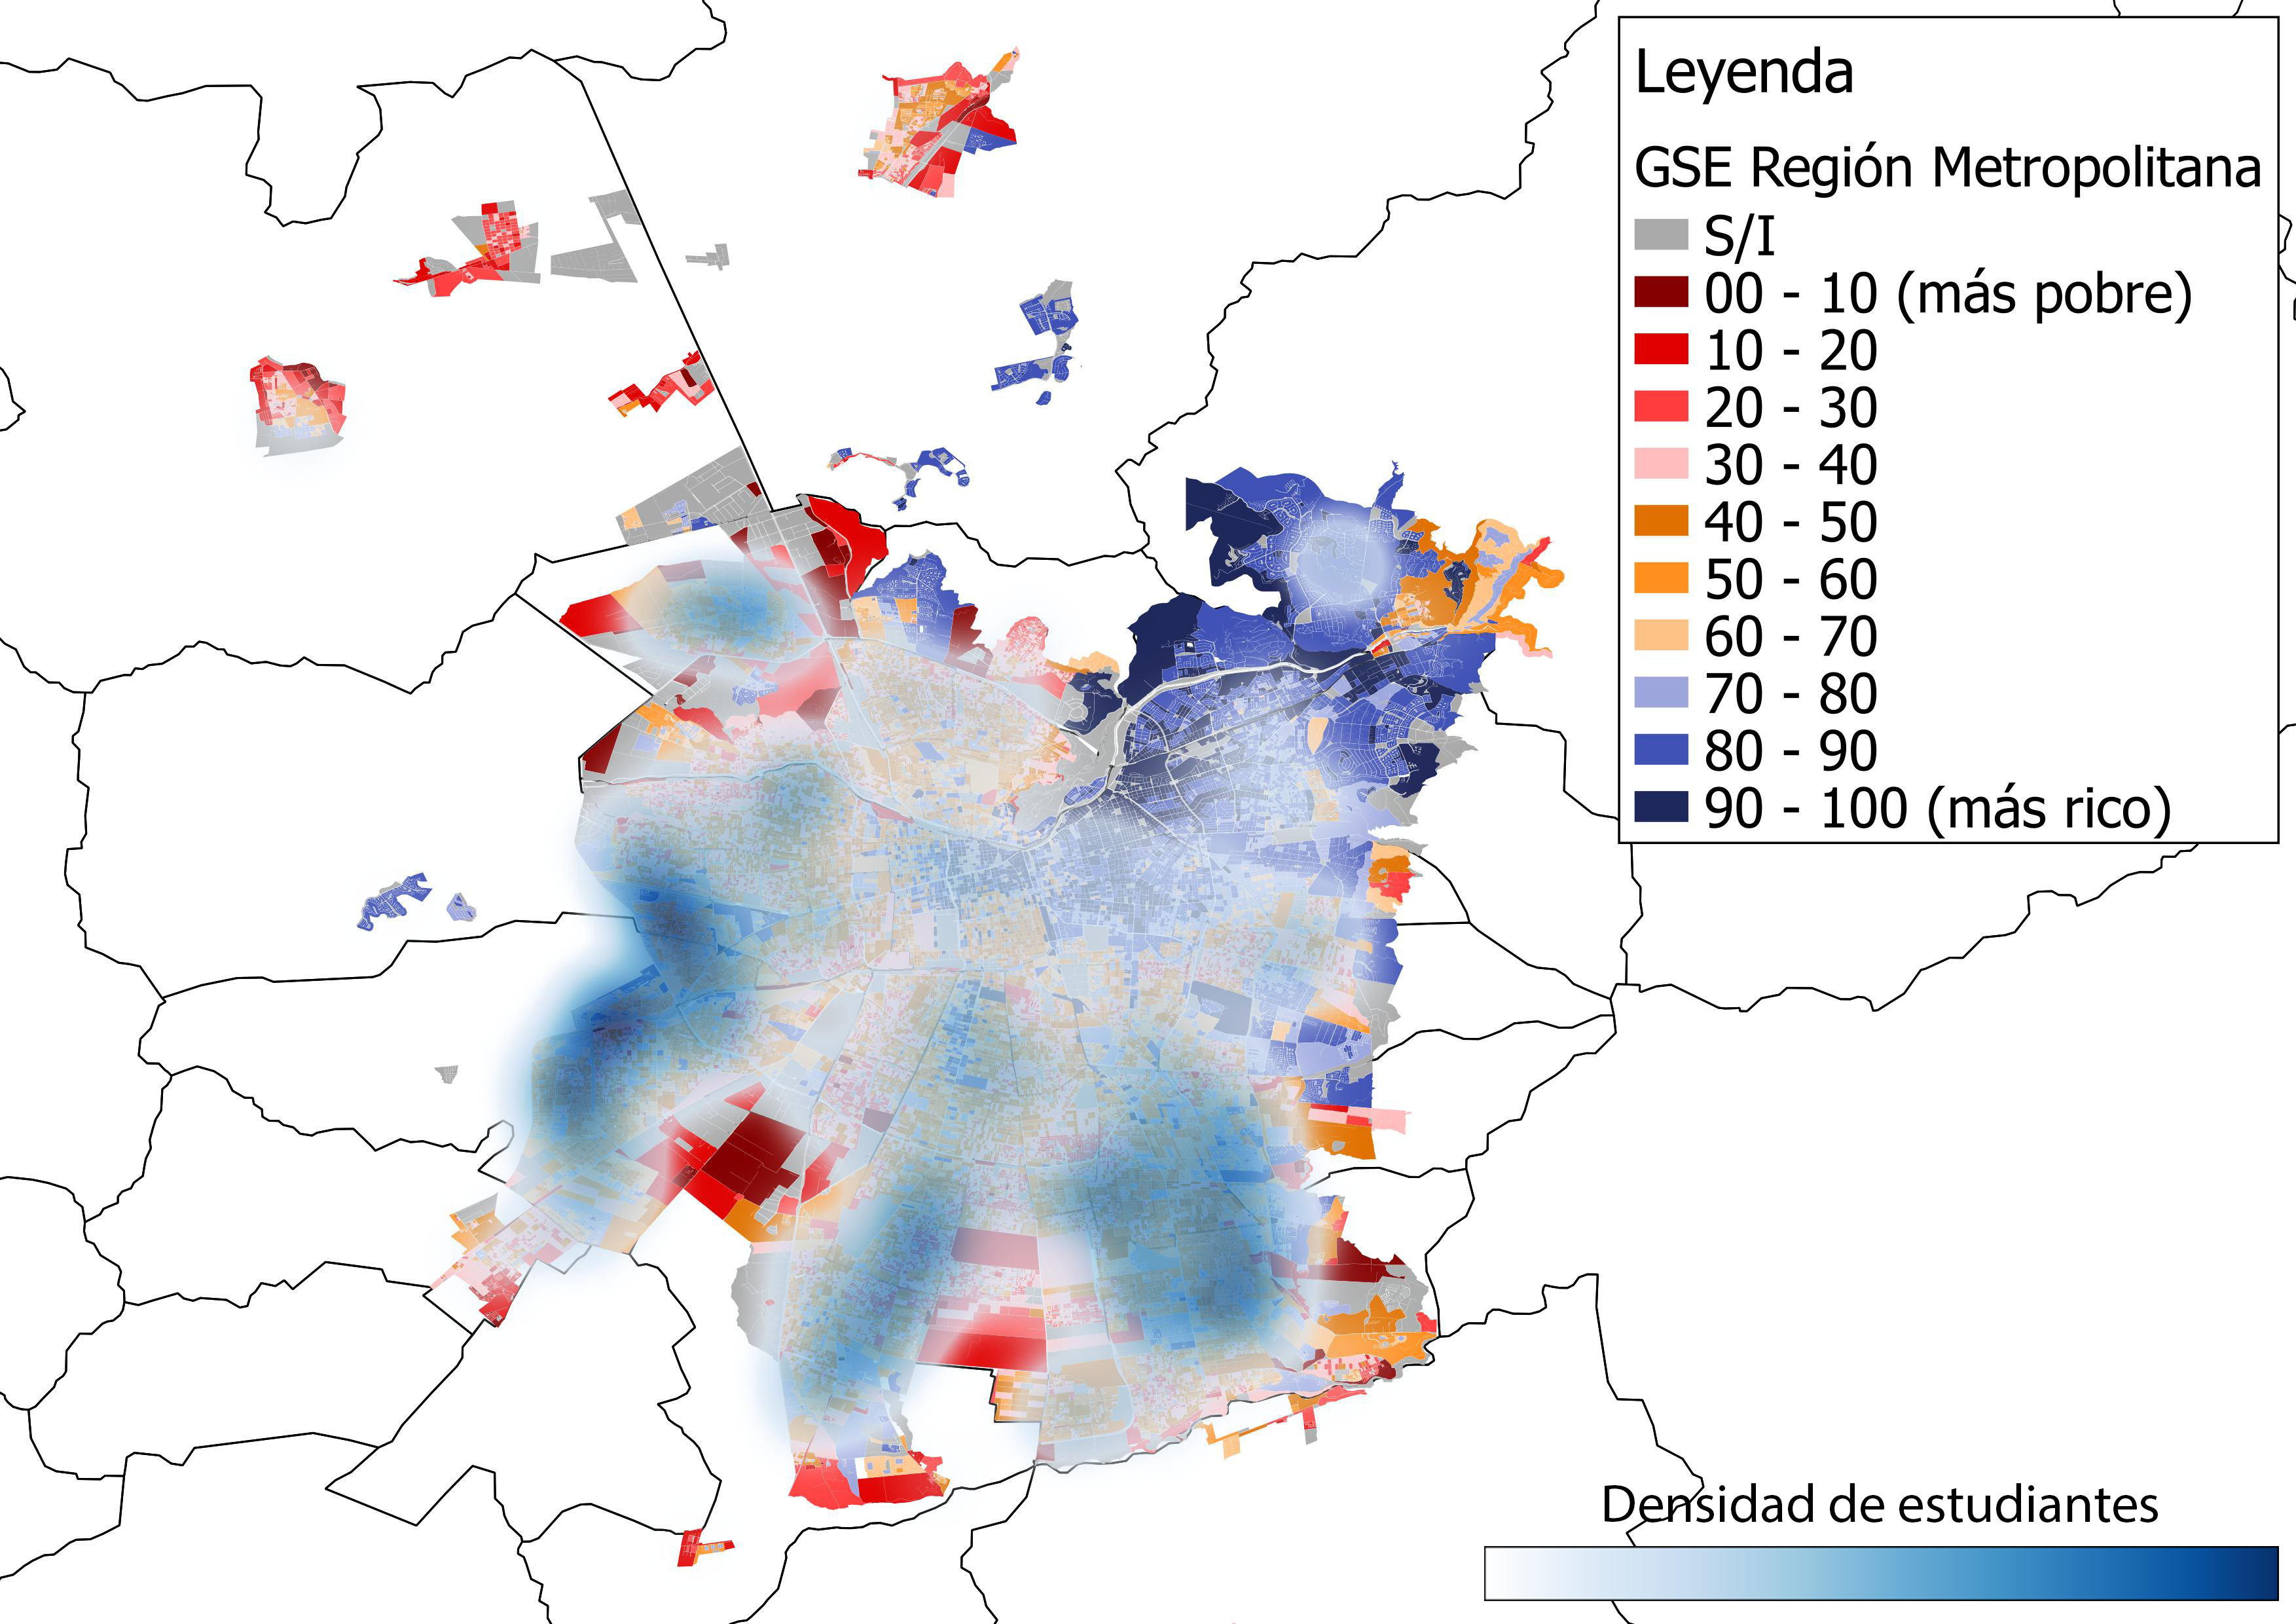
\includegraphics[width=7.5cm]{images/matriculas/E_SIN_2_final.jpg}}
  \subfloat[Matrículas en colegios de E\_TODOS\_SIN\_3.]{
   \label{f:}
    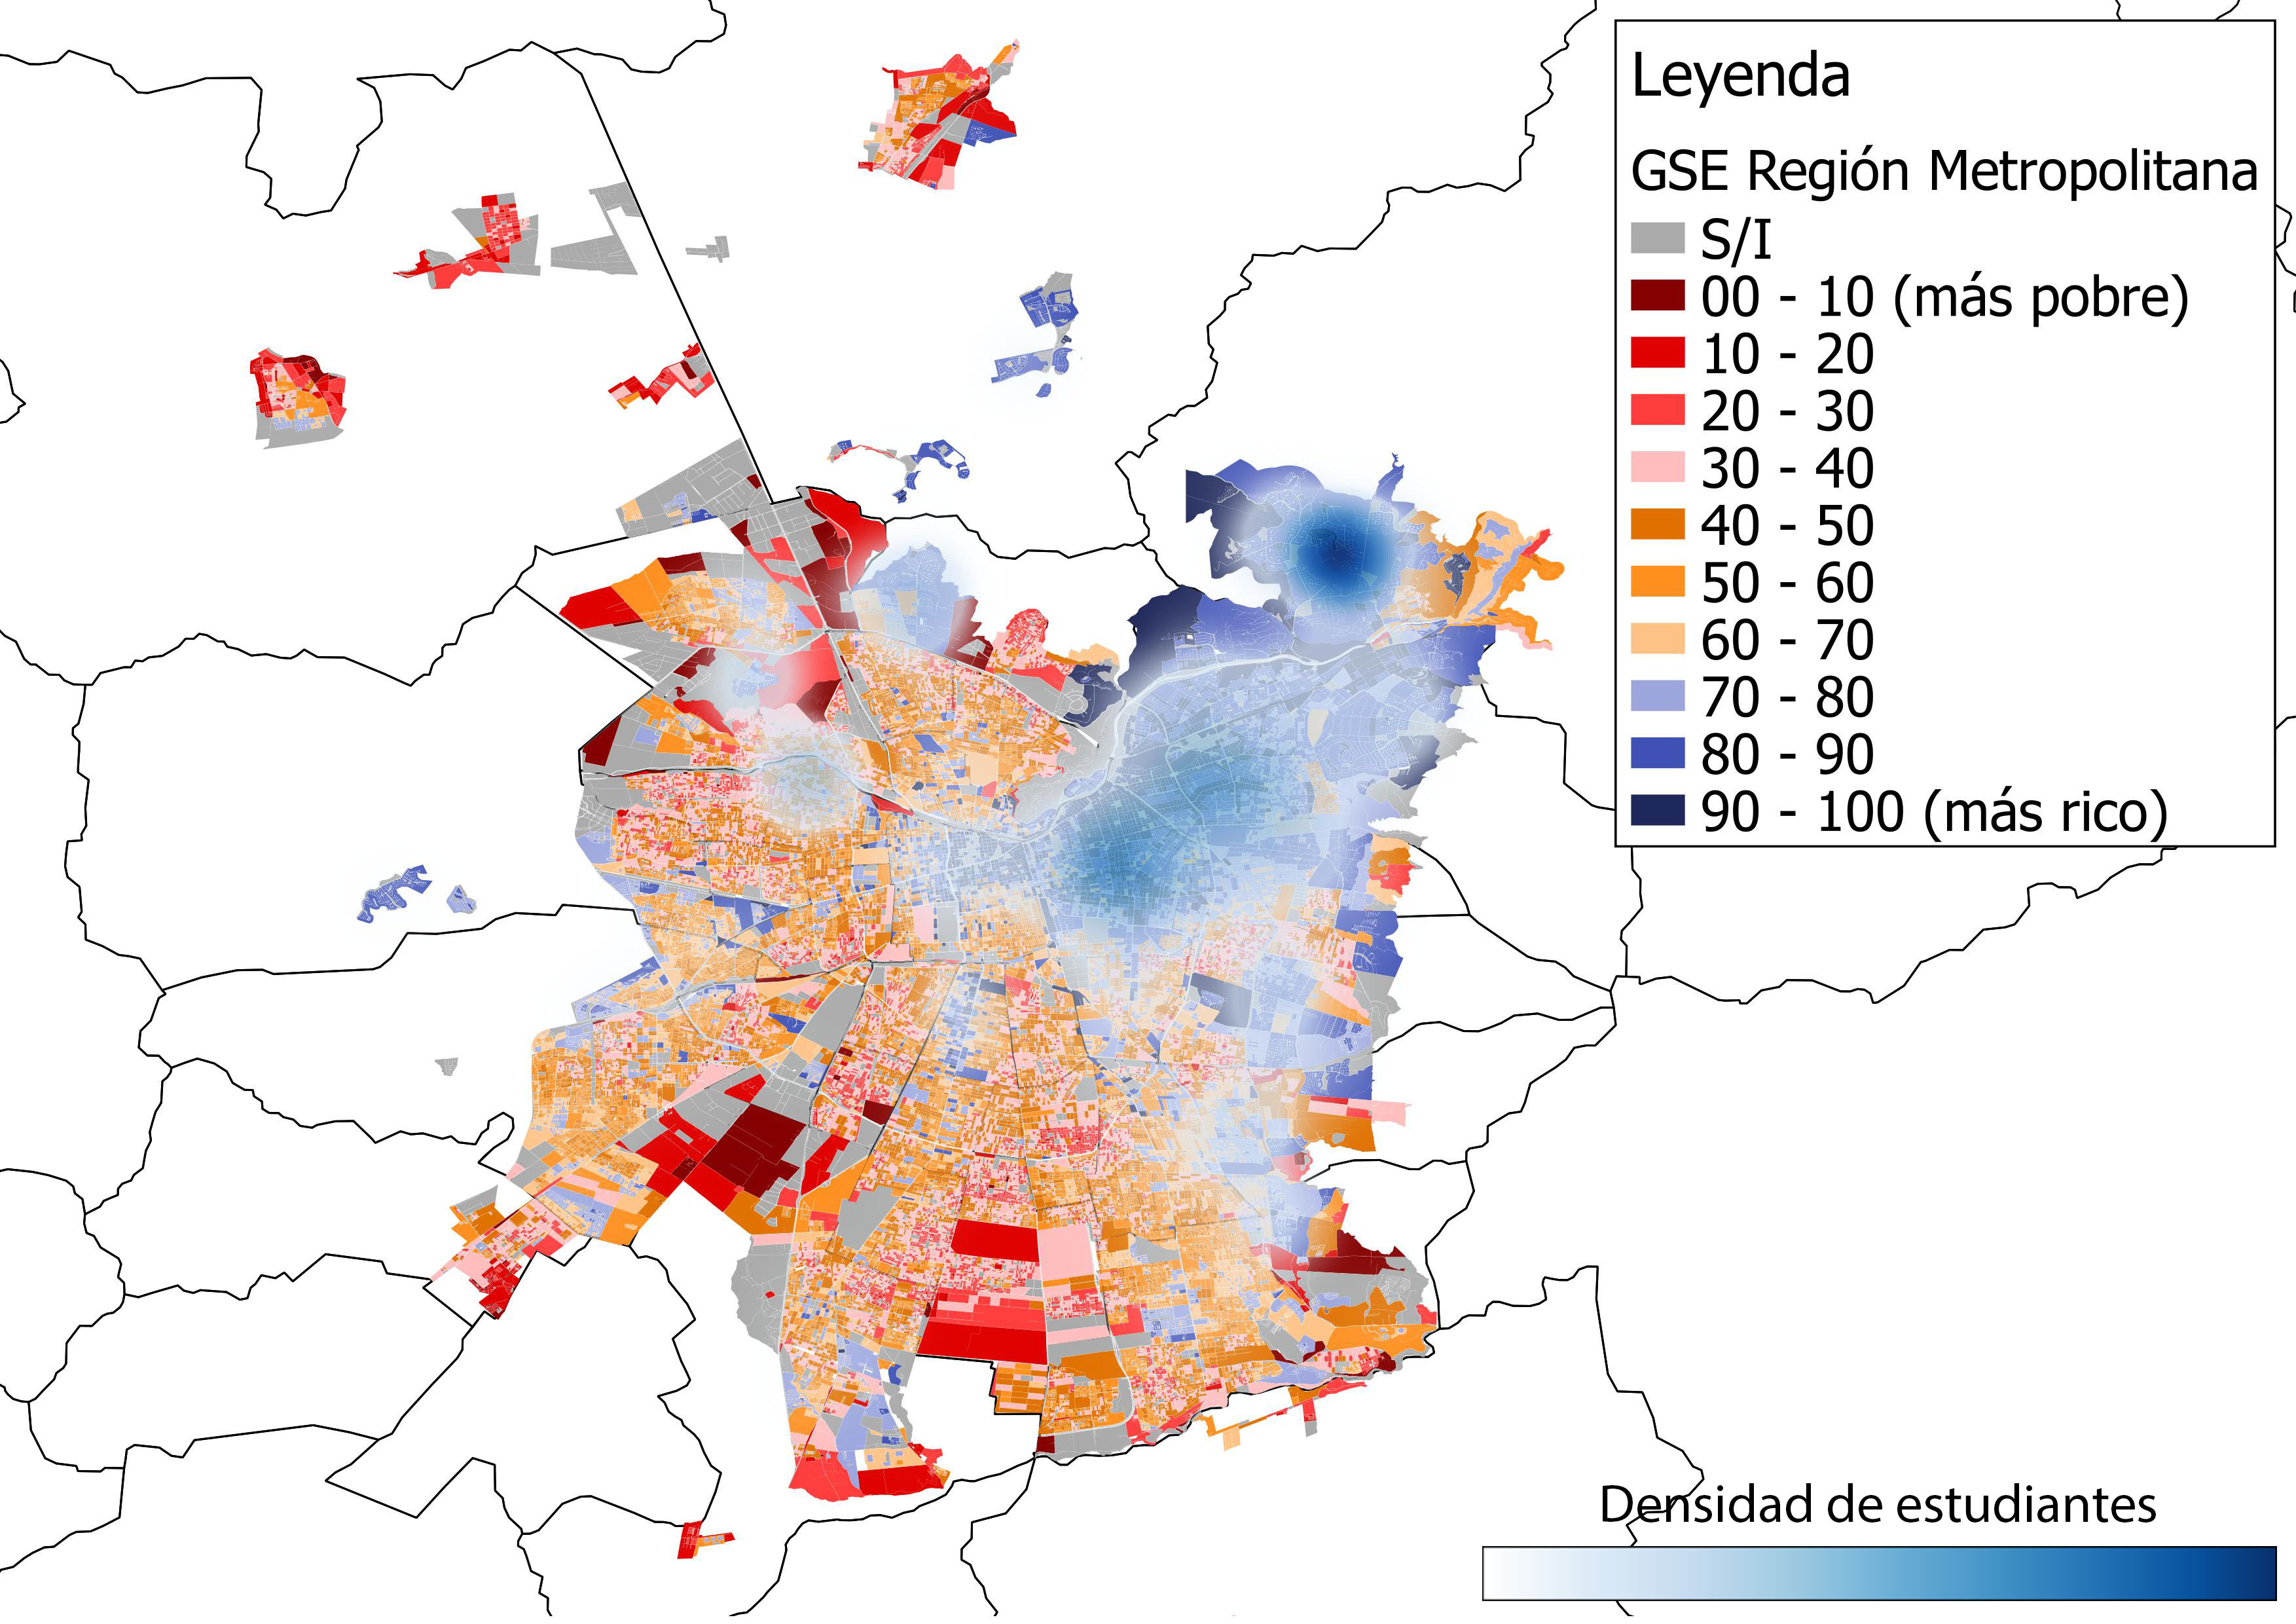
\includegraphics[width=7.5cm]{images/matriculas/E_SIN_3_final.jpg}}
 \caption{Mapas de calor de matrículas en clústers de establecimientos sobre mapa GSE de la Región Metropolitana.}
 \label{f:}
\end{figure}

\begin{figure}[h]
 \centering
  \subfloat[Matrículas clúster M\_TODAS\_SIN\_0.]{
   \label{f:}
    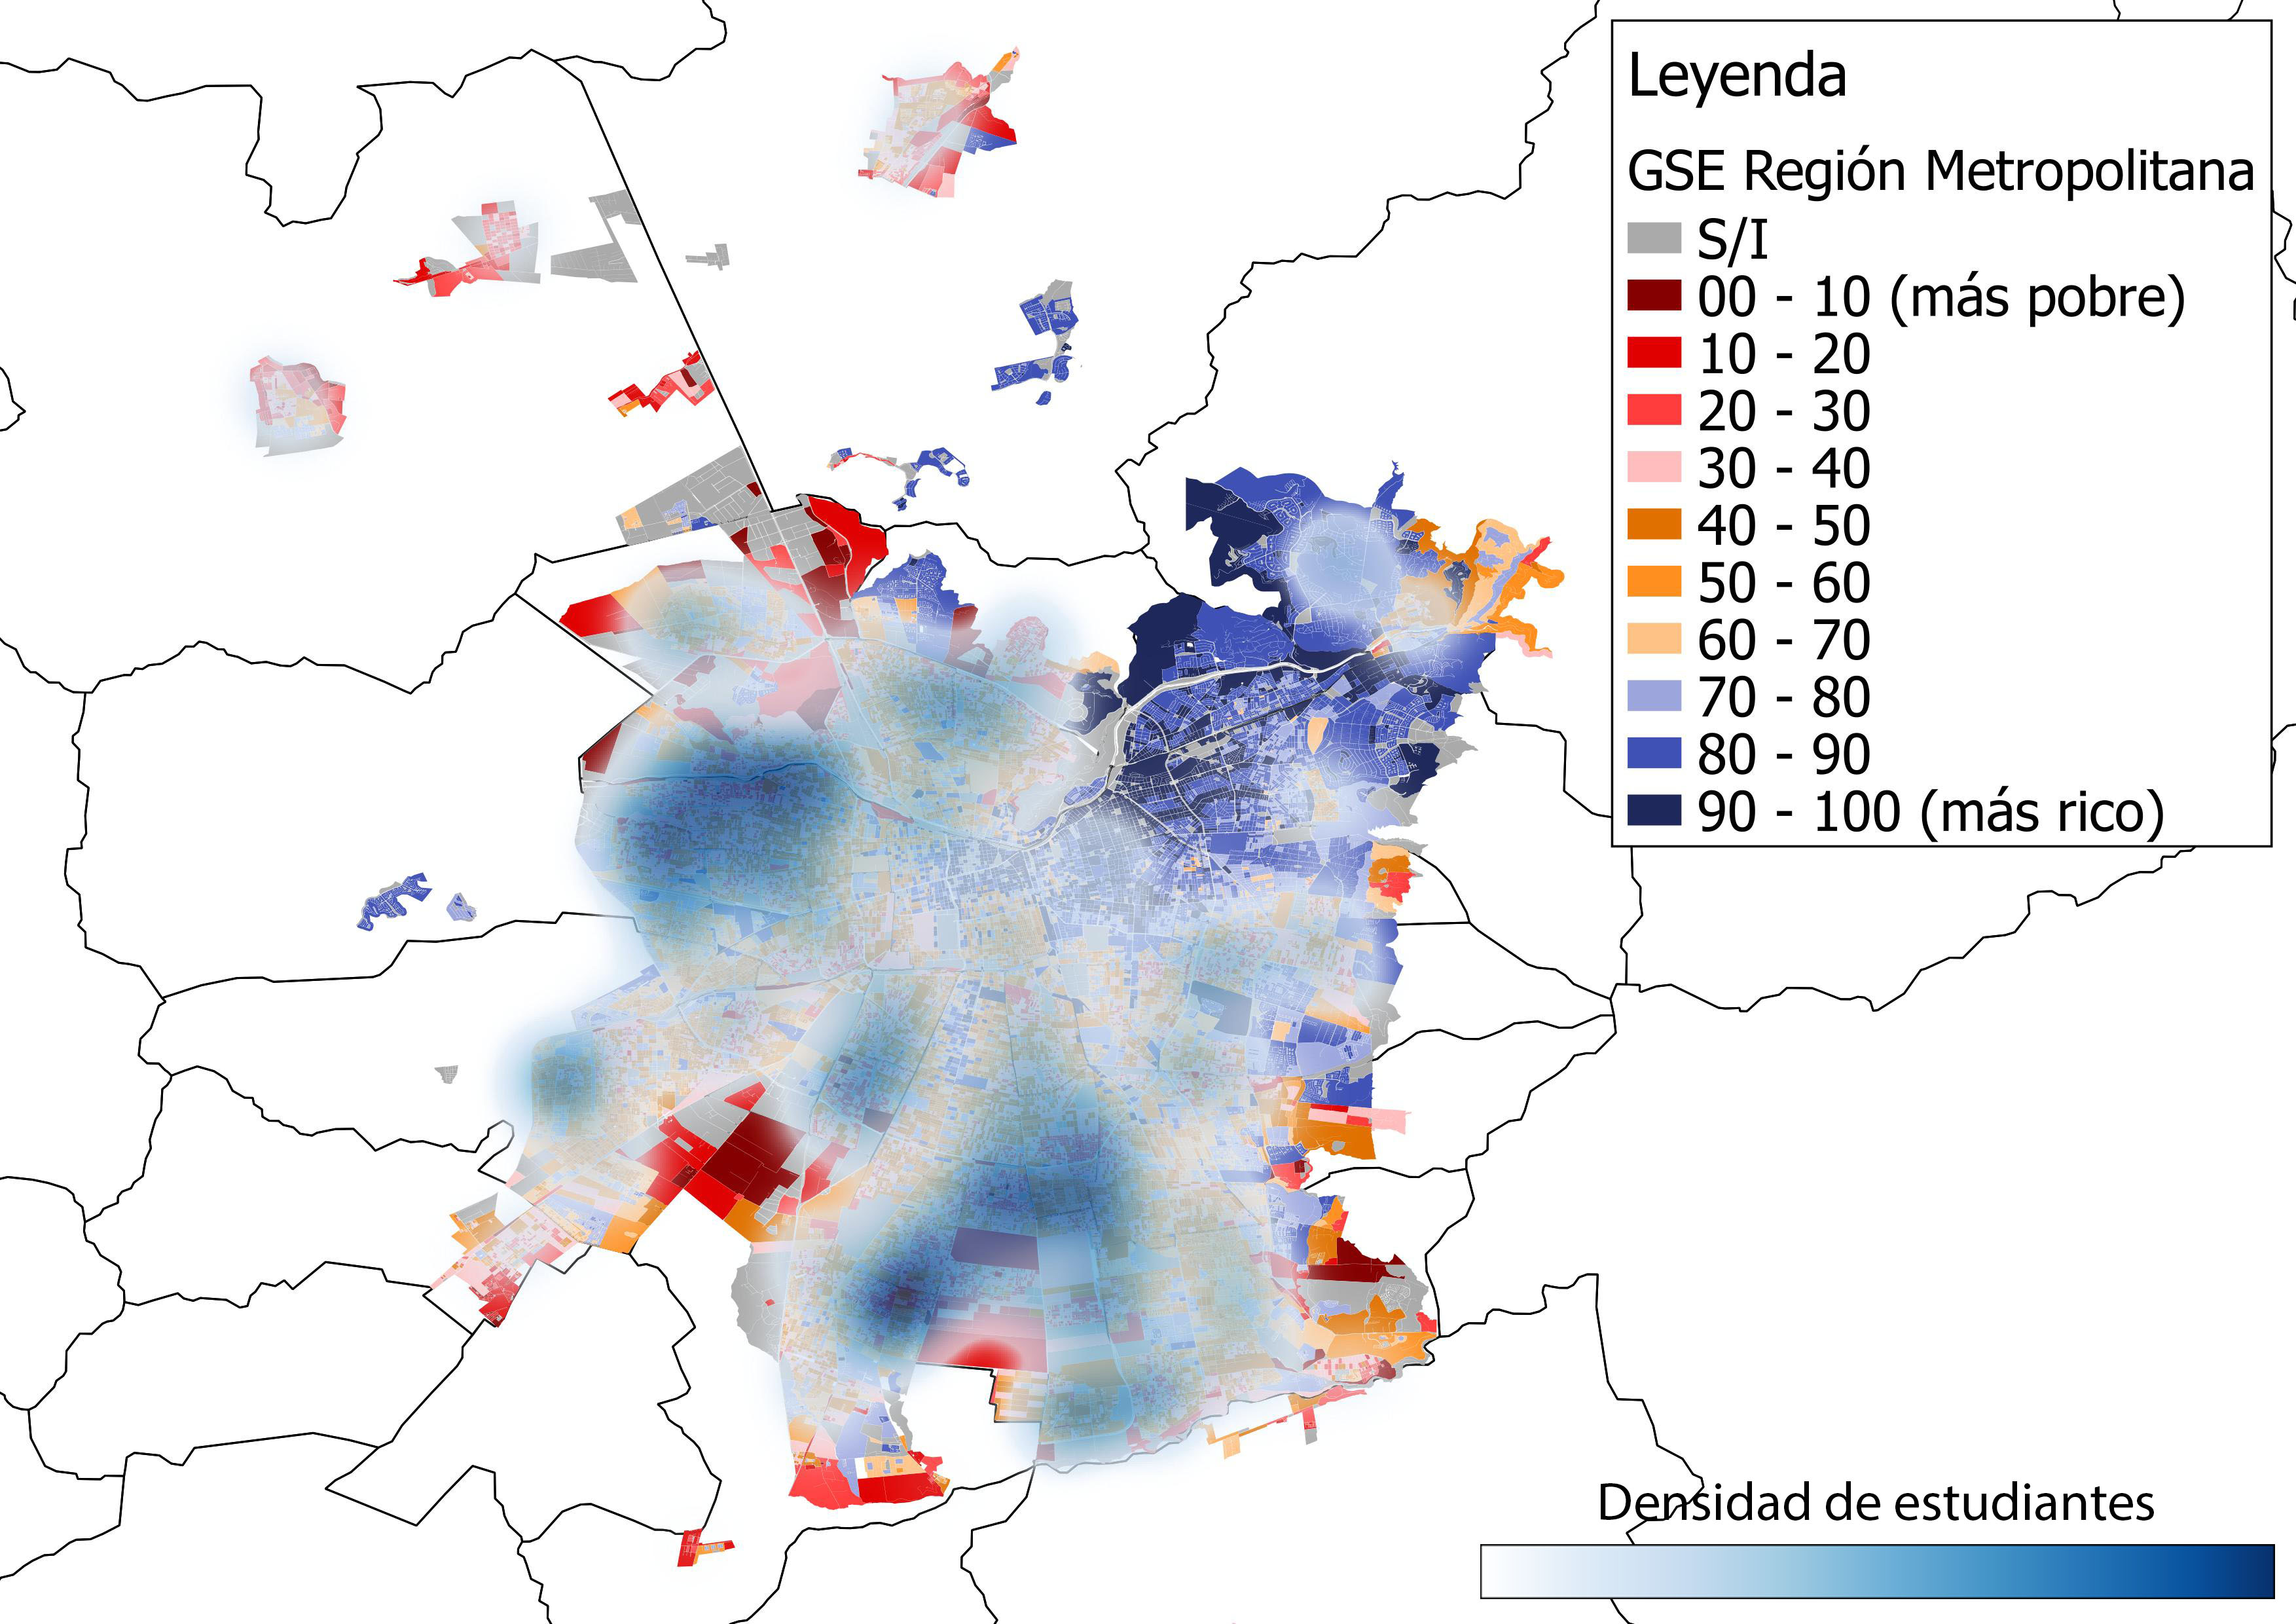
\includegraphics[width=7.5cm]{images/matriculas/M_SIN_0_final.jpg}}
  \subfloat[Matrículas clúster M\_TODAS\_SIN\_1.]{
   \label{f:}
    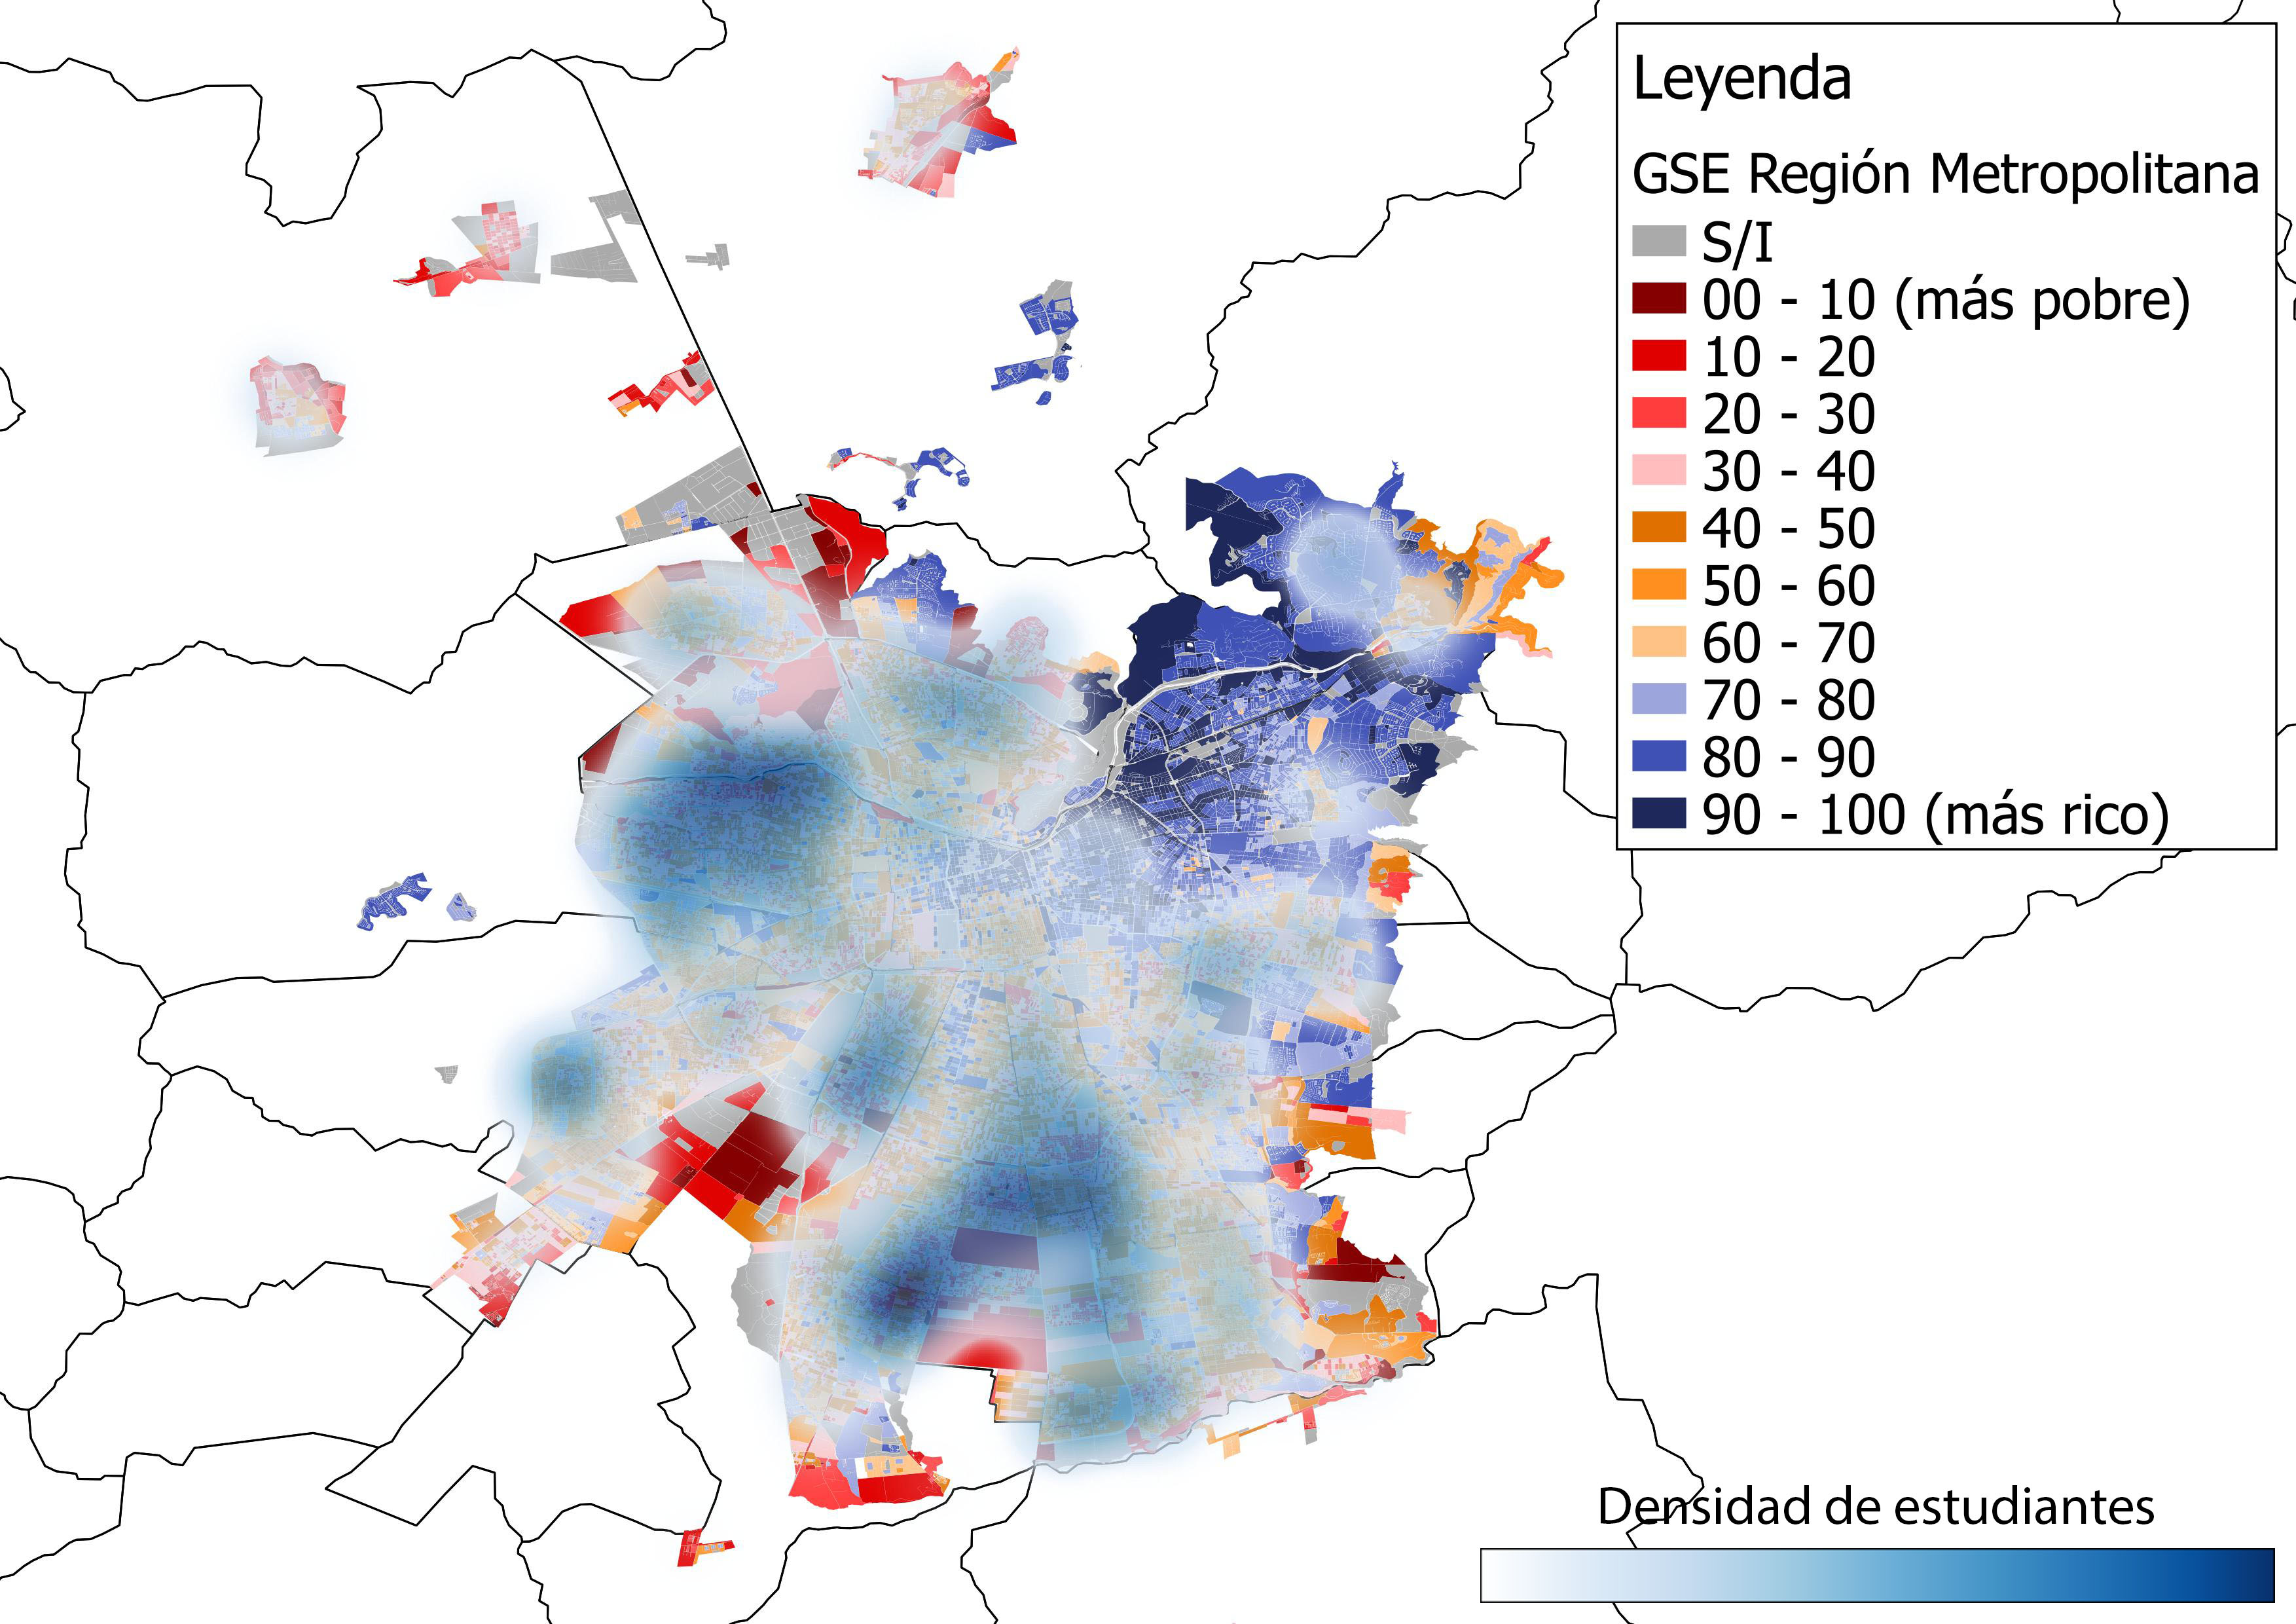
\includegraphics[width=7.5cm]{images/matriculas/M_SIN_1_final.jpg}}\hspace{1mm}
  \subfloat[Matrículas clúster M\_TODAS\_SIN\_2.]{
   \label{f:}
    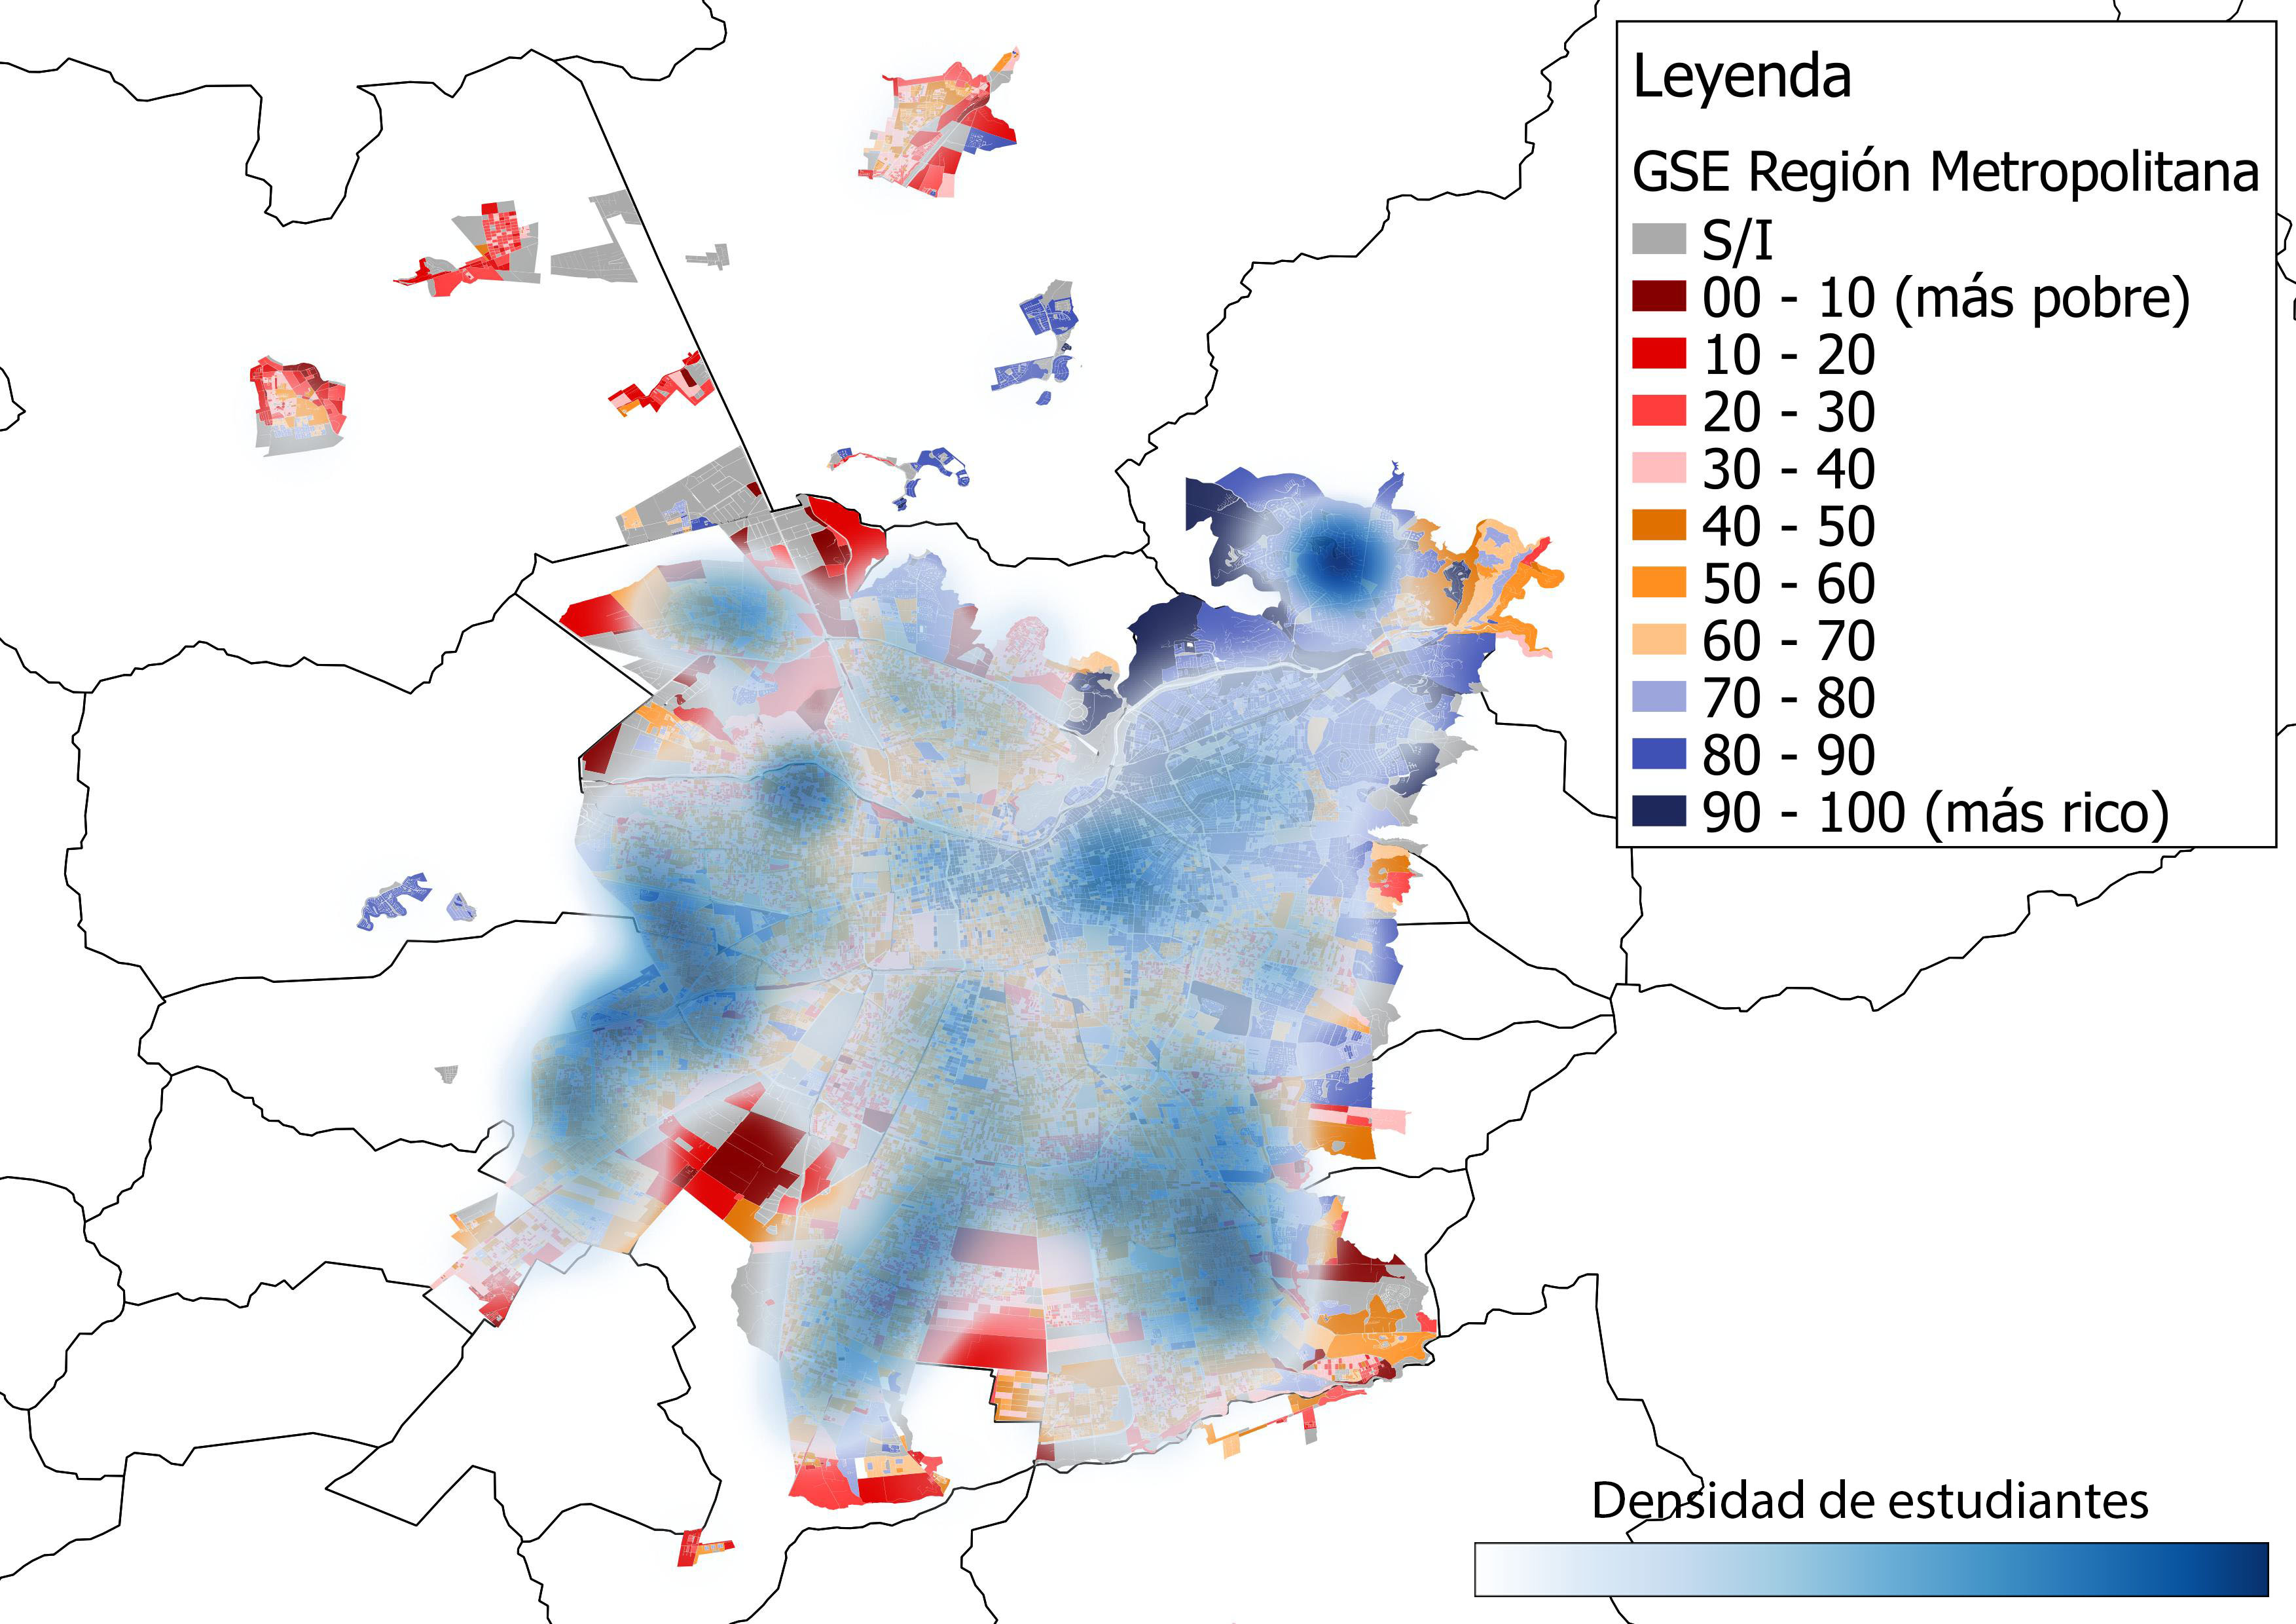
\includegraphics[width=7.5cm]{images/matriculas/M_SIN_2_final.jpg}}
  \subfloat[Matrículas clúster M\_TODAS\_SIN\_3.]{
   \label{f:}
    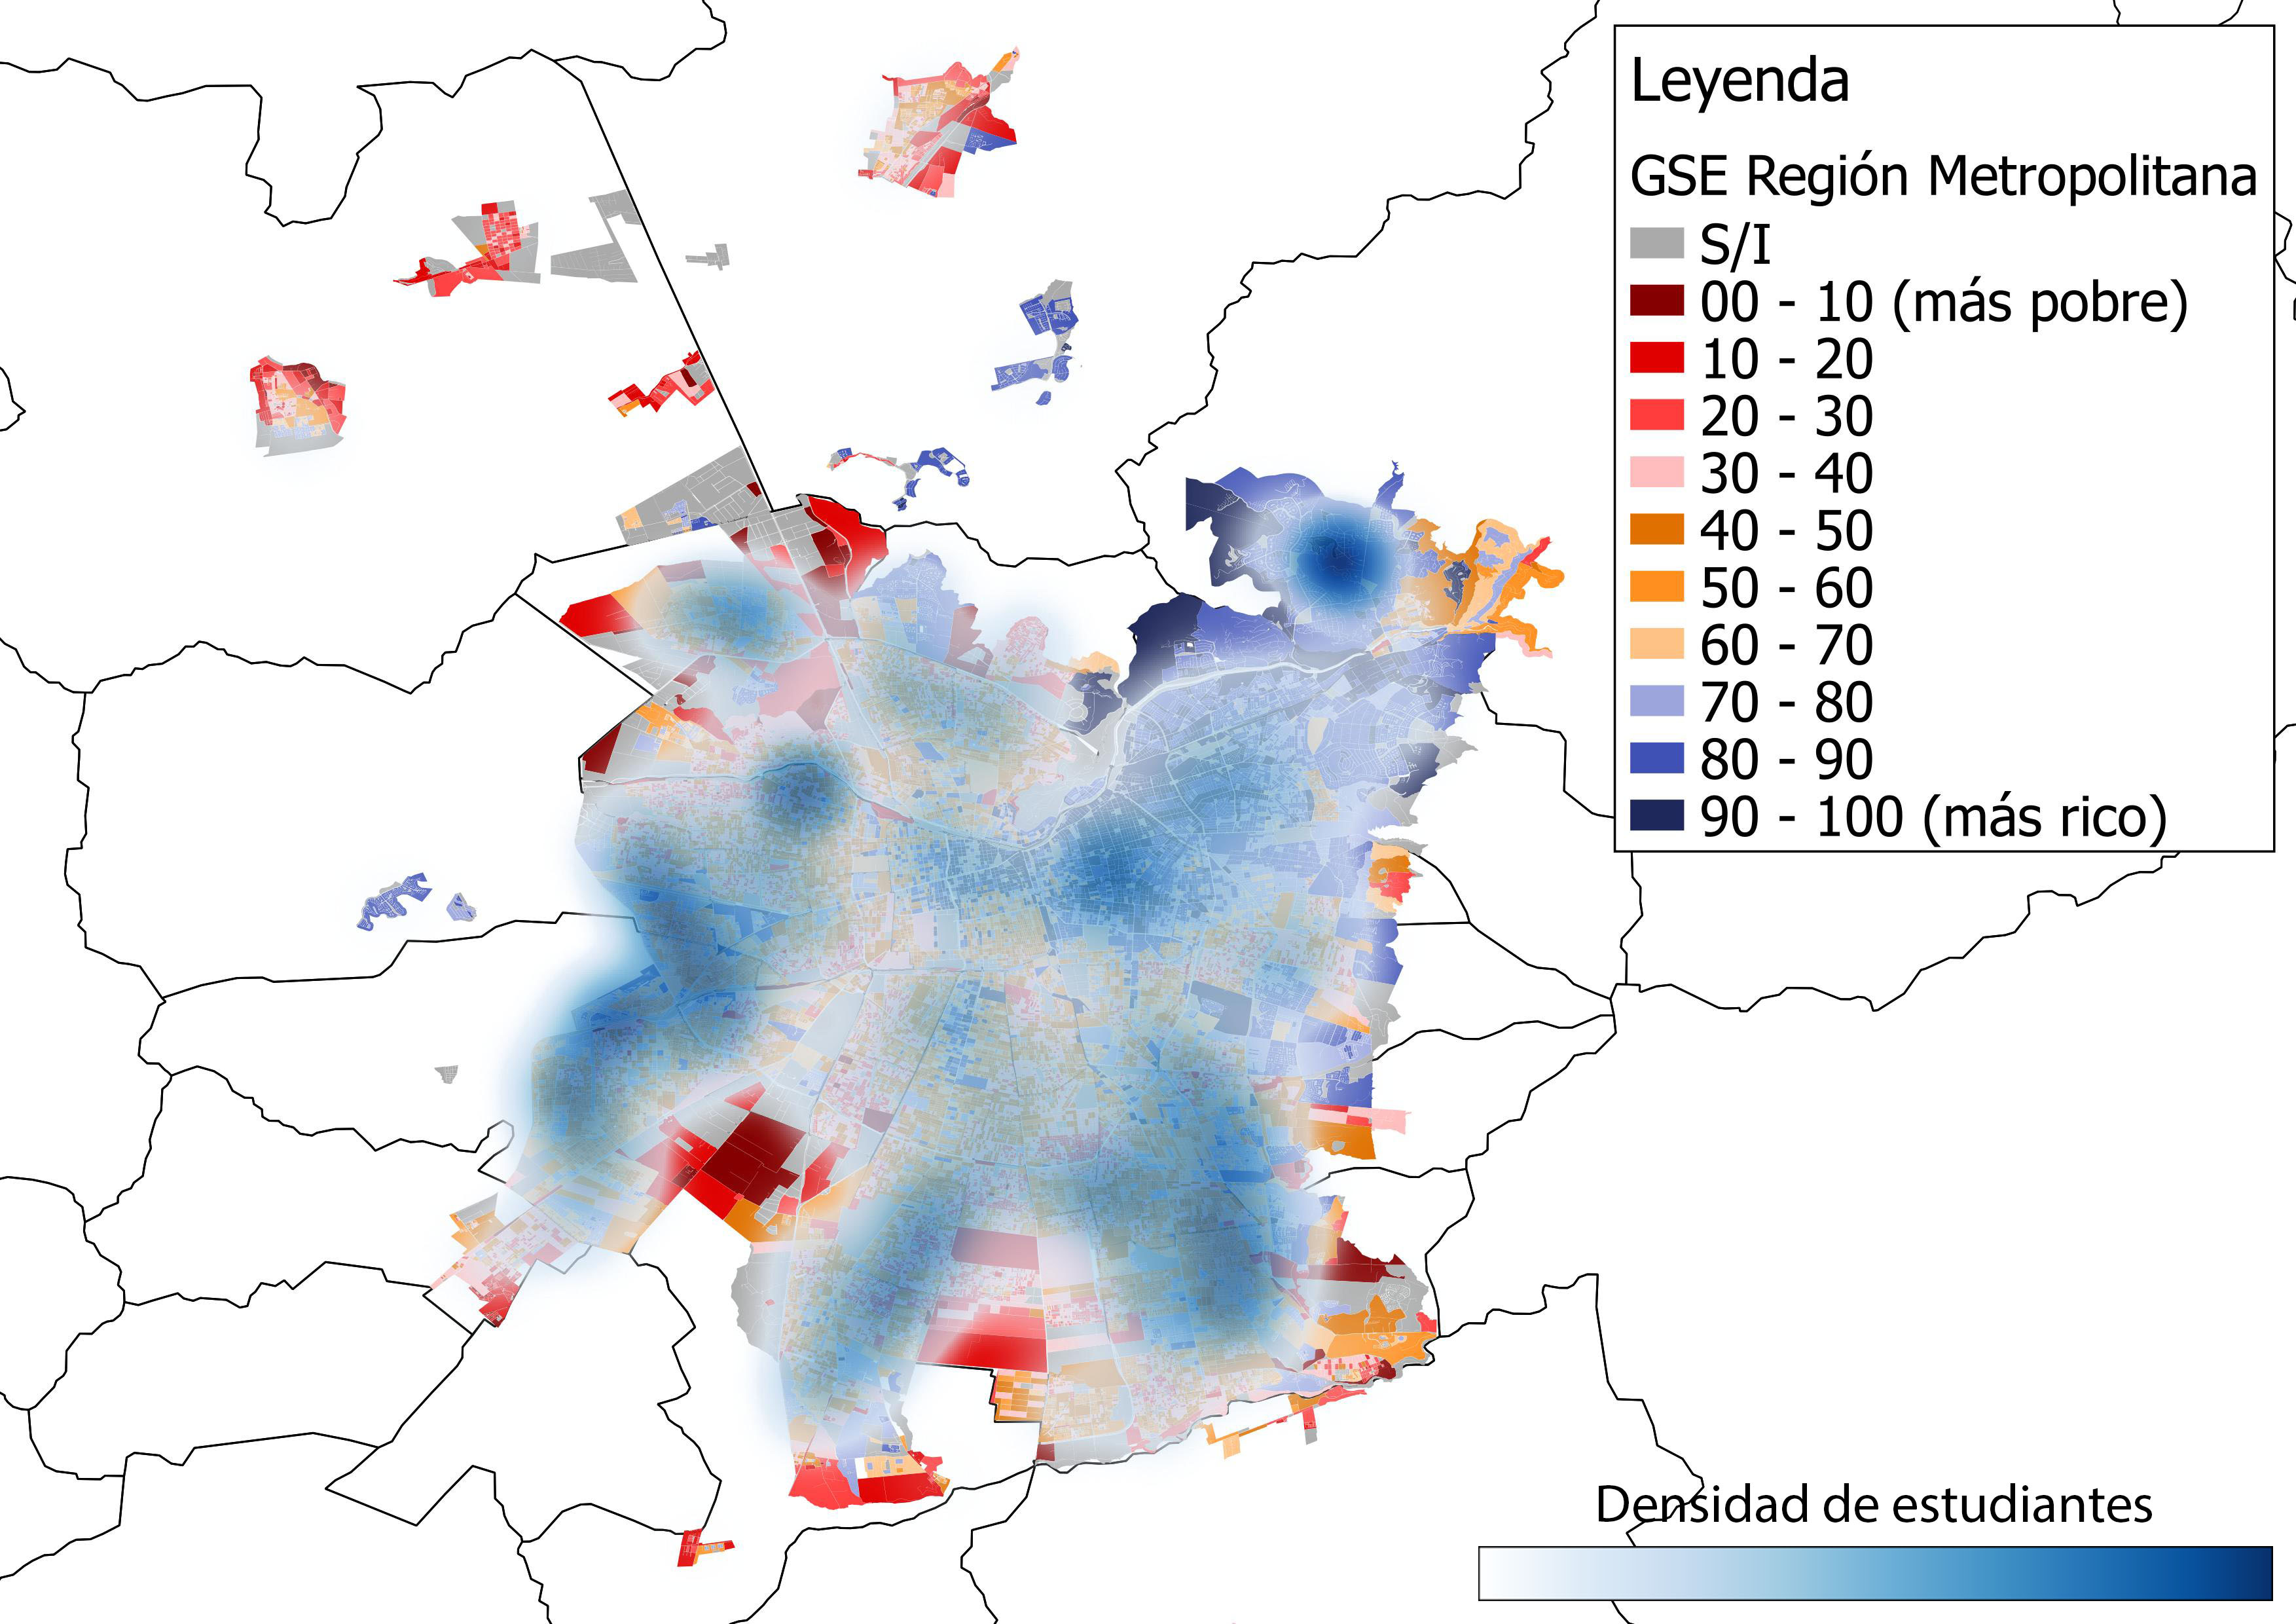
\includegraphics[width=7.5cm]{images/matriculas/M_SIN_3_final.jpg}}
 \caption{Mapas de calor de clústers de matrículas sobre mapa GSE de la Región Metropolitana.}
 \label{f:}
\end{figure}

\begin{figure}[h]
 \centering
  \subfloat[Matrículas en colegios de E\_TODOS\_CON\_0.]{
   \label{f:}
    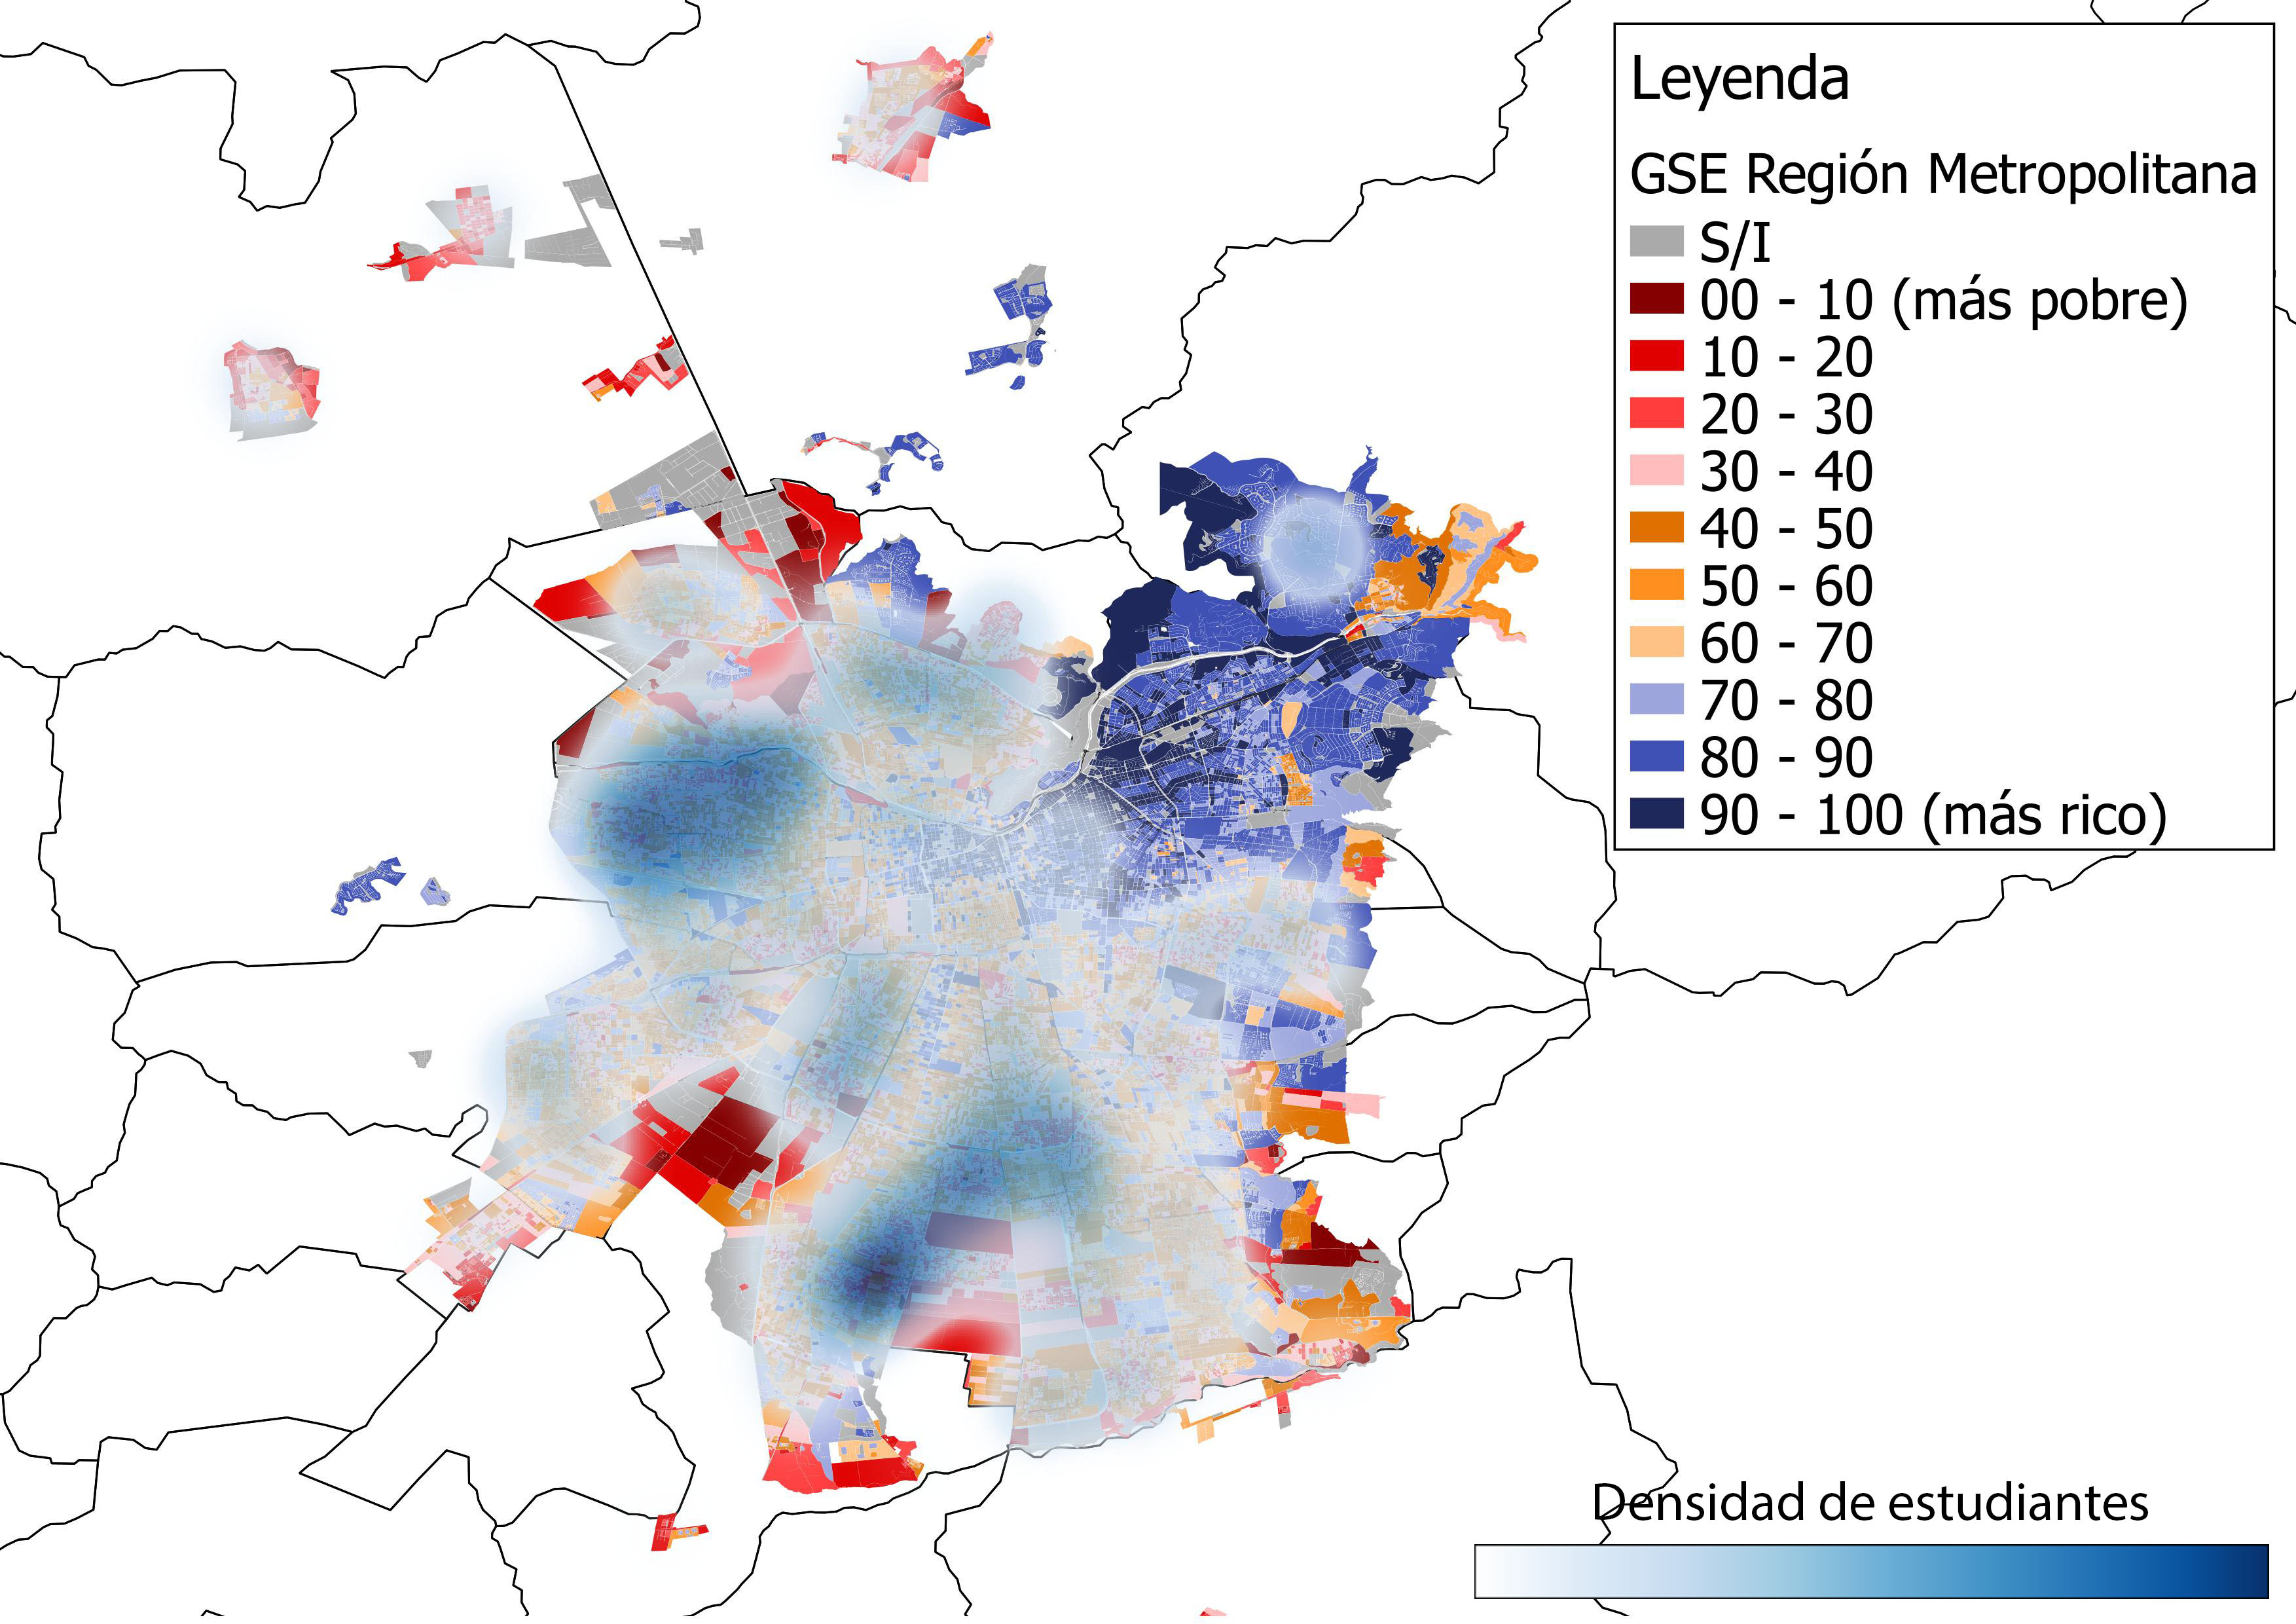
\includegraphics[width=7.5cm]{images/matriculas/E_CON_0_final.jpg}}
  \subfloat[Matrículas en colegios de E\_TODOS\_CON\_1.]{
   \label{f:}
    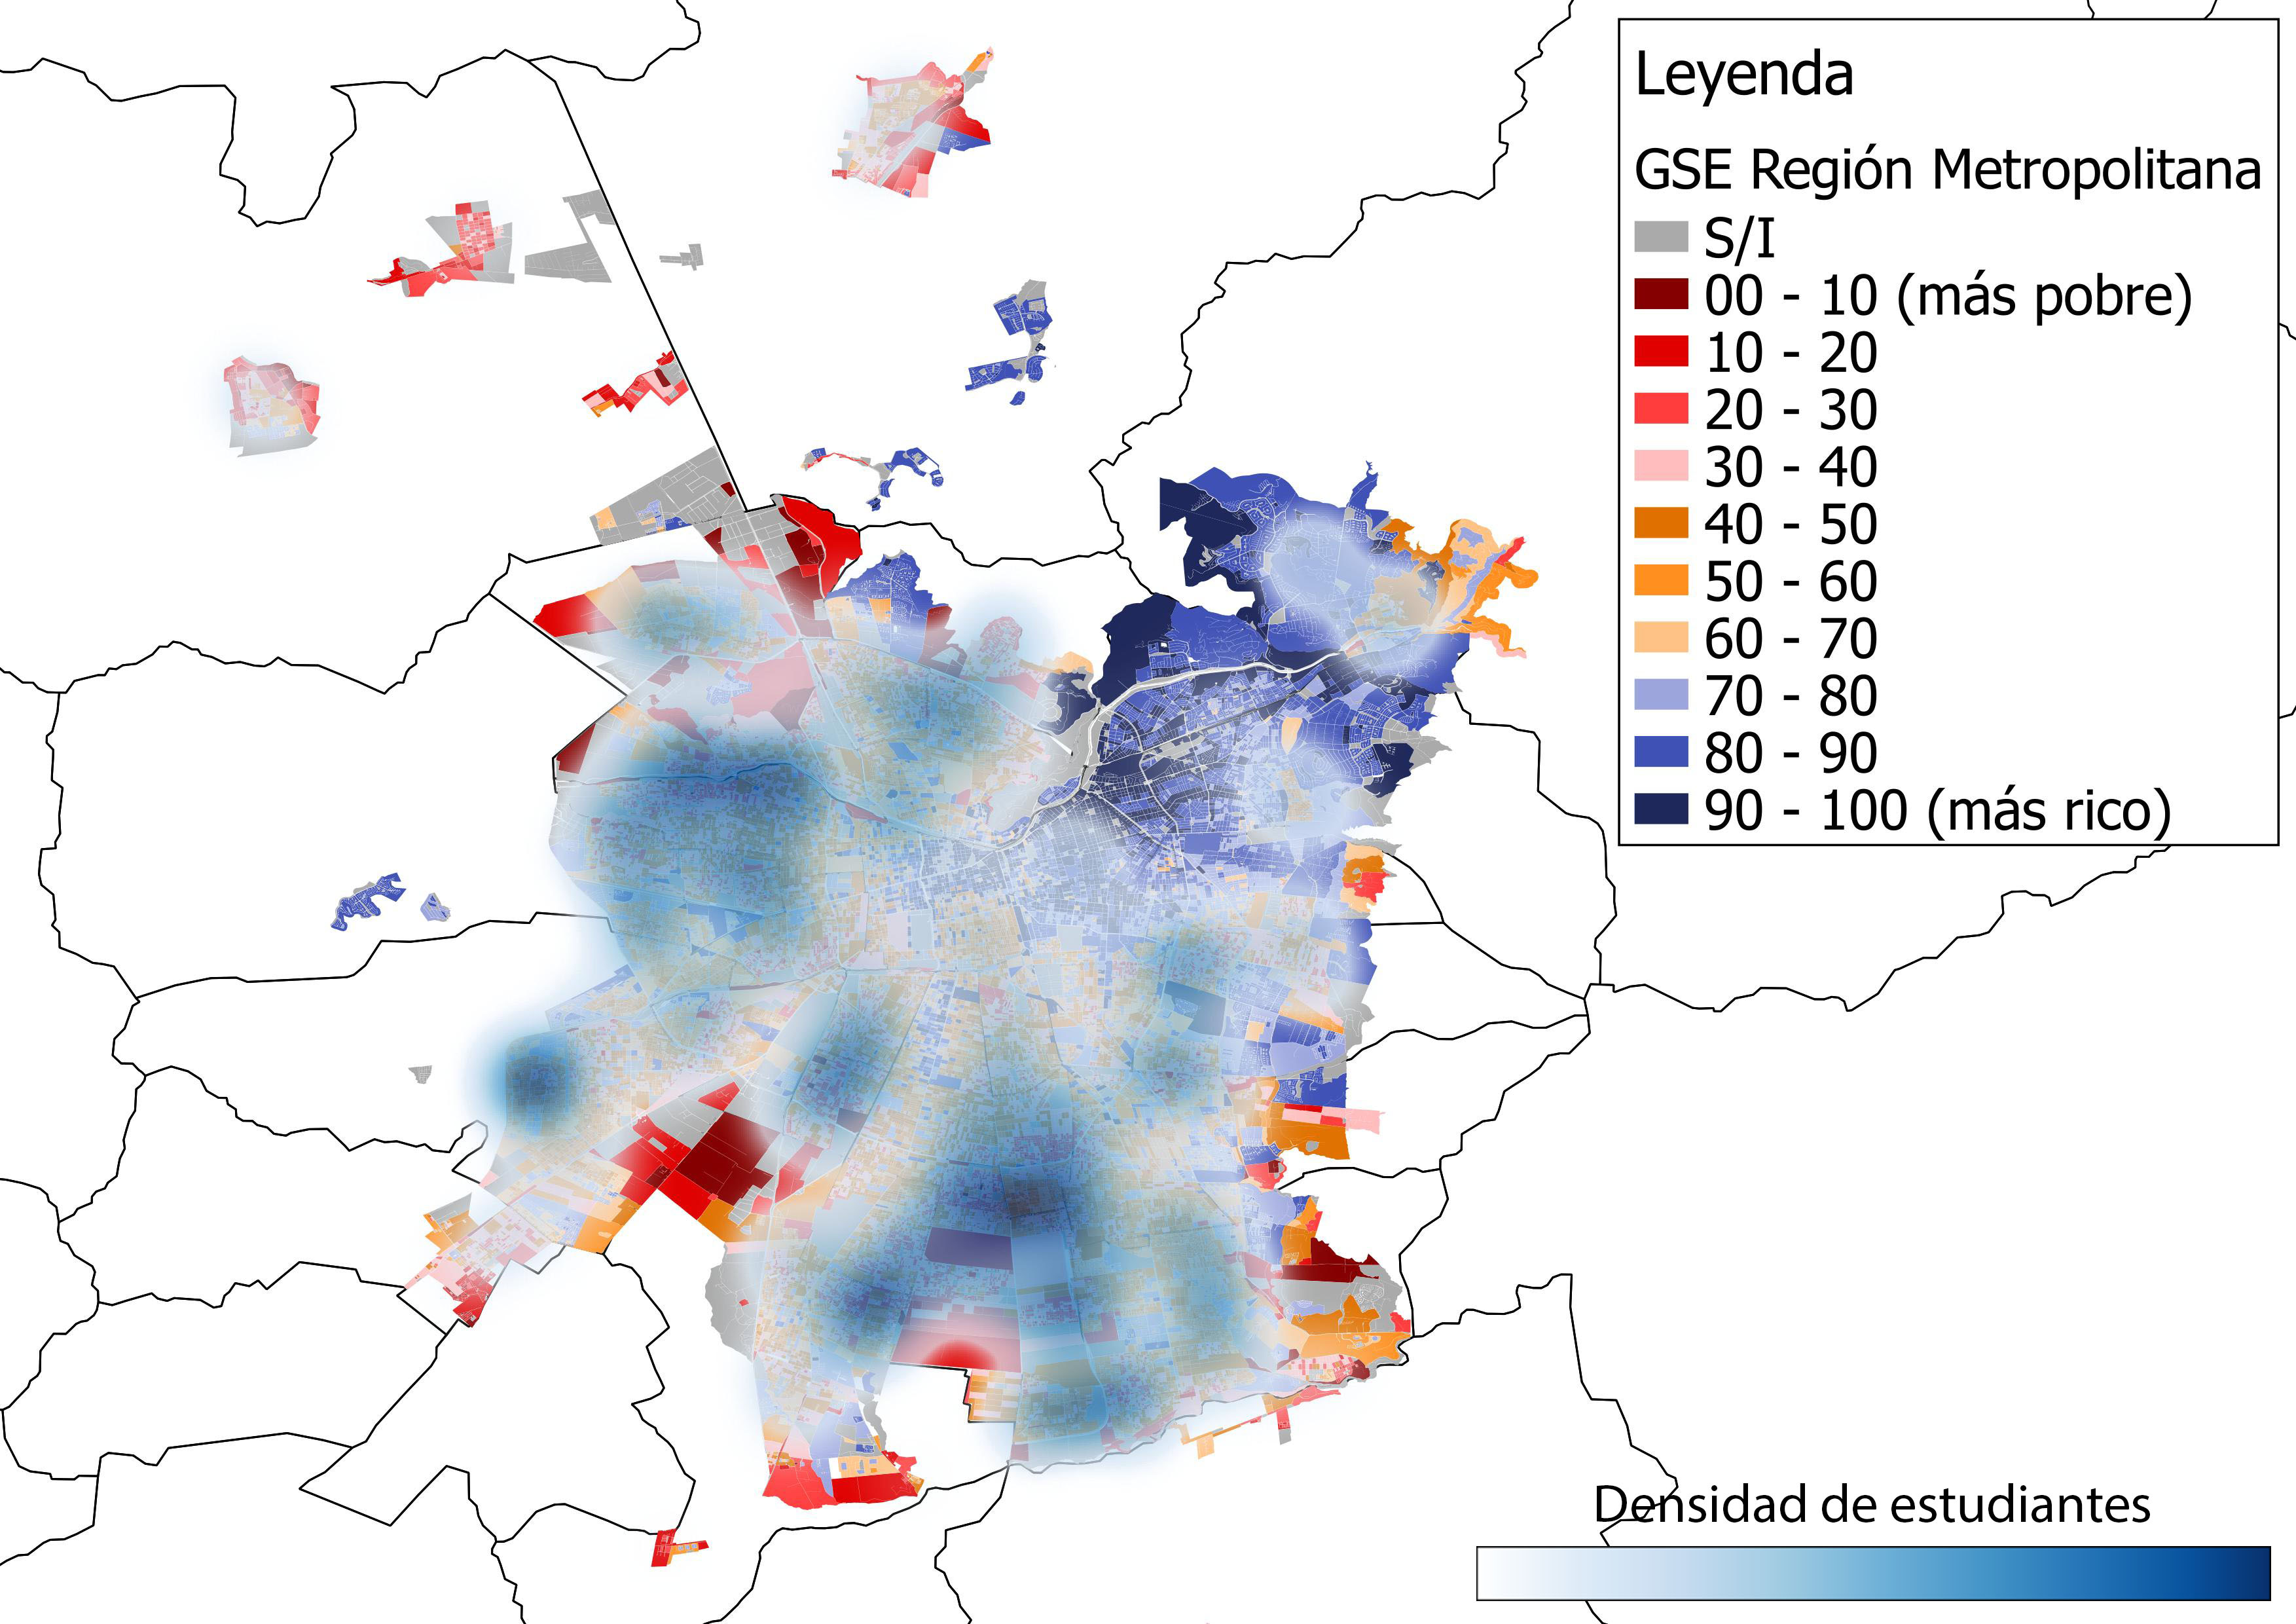
\includegraphics[width=7.5cm]{images/matriculas/E_CON_1_final.jpg}}\hspace{1mm}
  \subfloat[Matrículas en colegios de E\_TODOS\_CON\_2.]{
   \label{f:}
    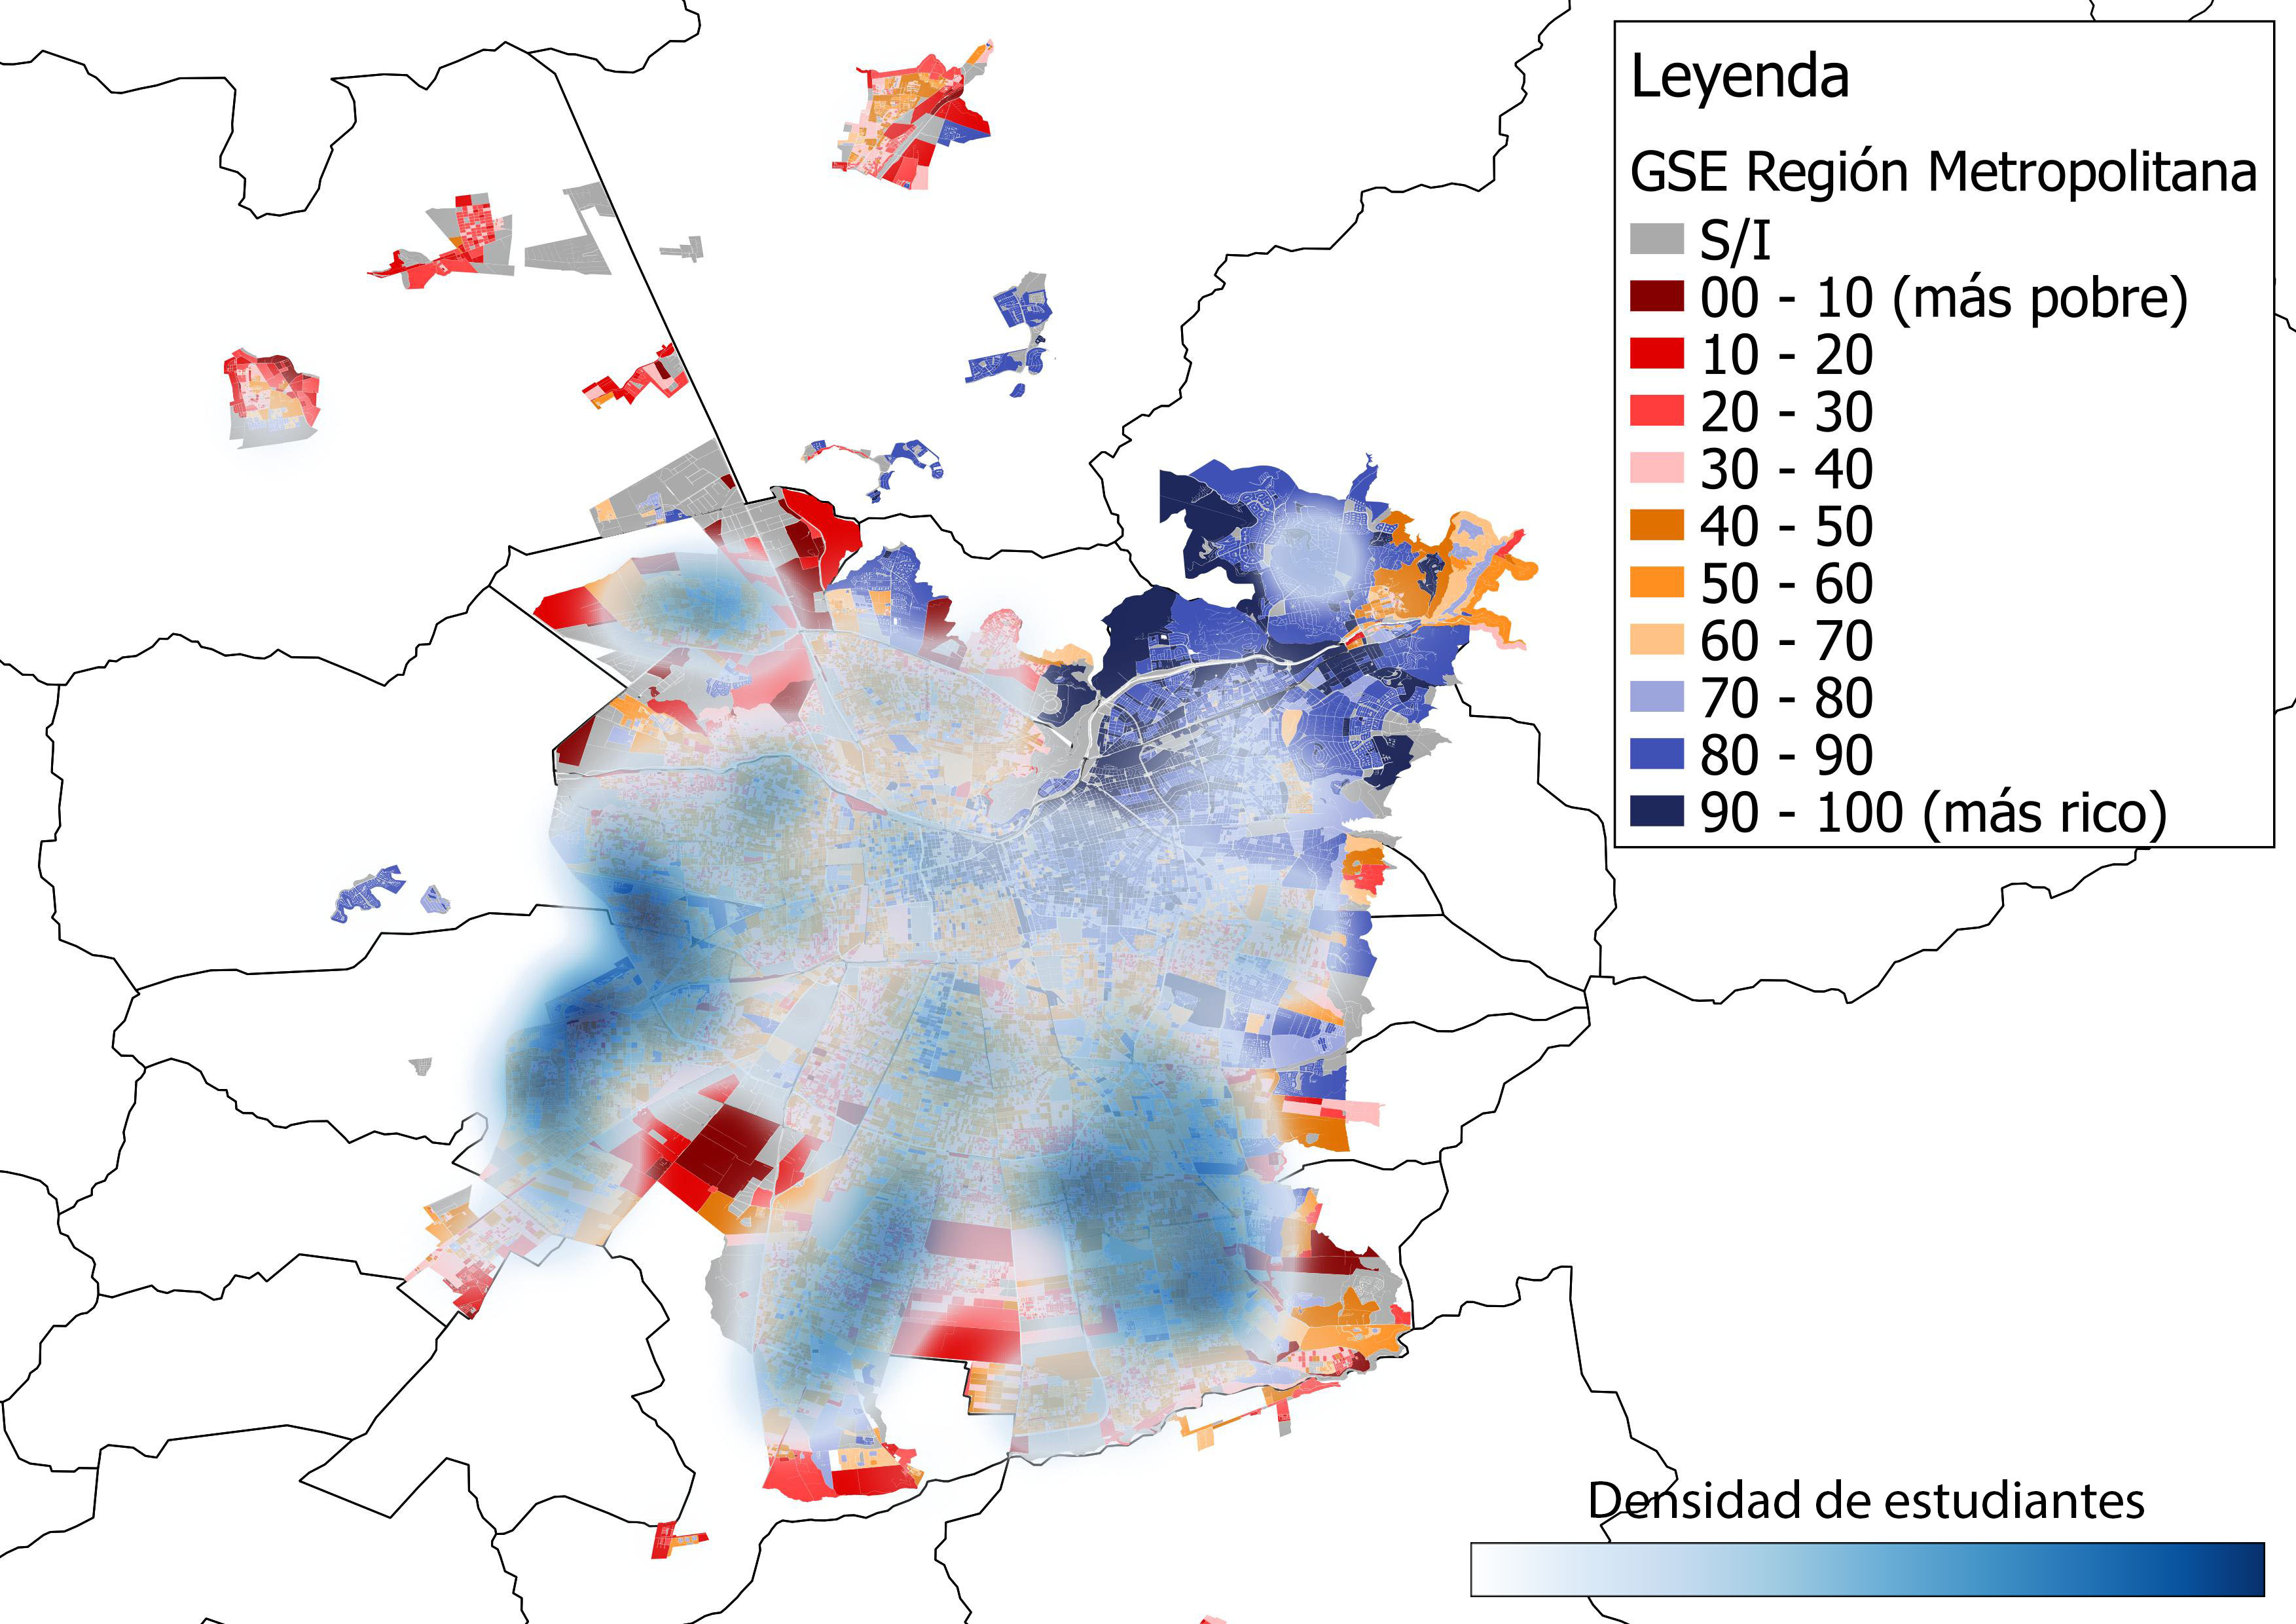
\includegraphics[width=7.5cm]{images/matriculas/E_CON_2_final.jpg}}
  \subfloat[Matrículas en colegios de E\_TODOS\_CON\_3.]{
   \label{f:}
    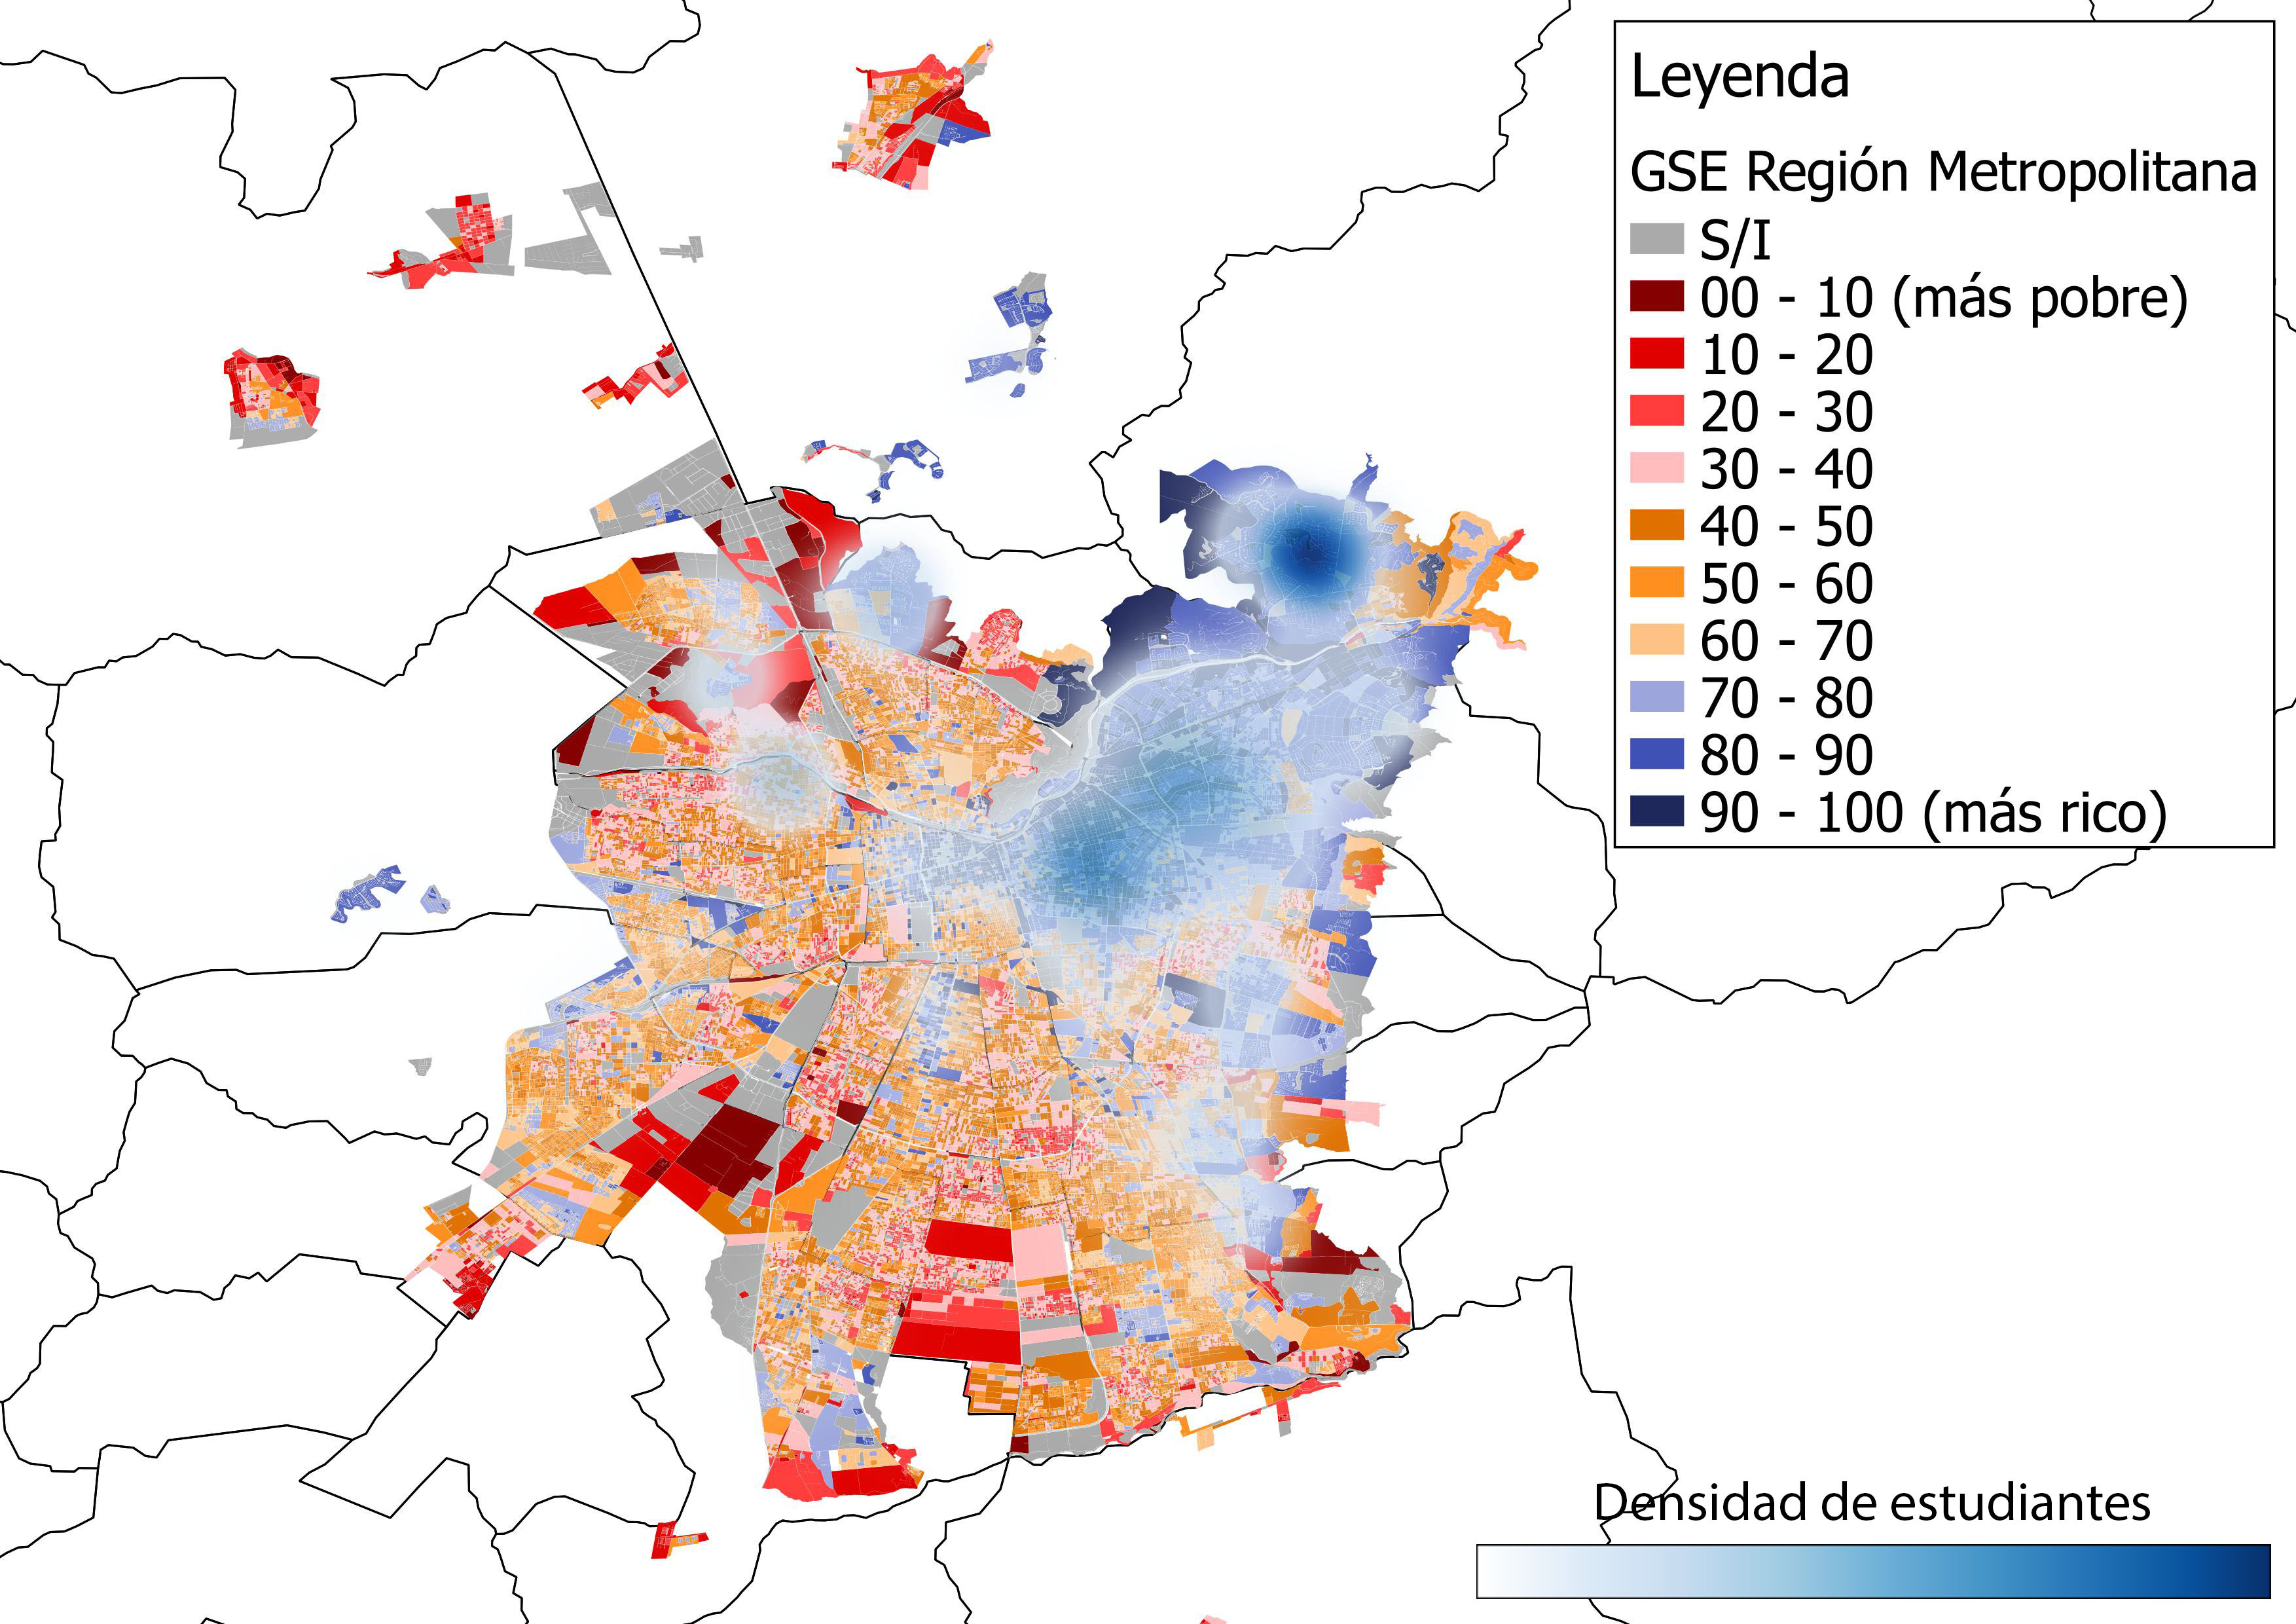
\includegraphics[width=7.5cm]{images/matriculas/E_CON_3_final.jpg}}
 \caption{Mapas de calor de matrículas (con atributos relacionales) en clústers de establecimientos sobre mapa GSE de la Región Metropolitana.}
 \label{f:}
\end{figure}

\begin{figure}[h]
 \centering
  \subfloat[Matrículas clúster M\_TODAS\_CON\_0.]{
   \label{f:}
    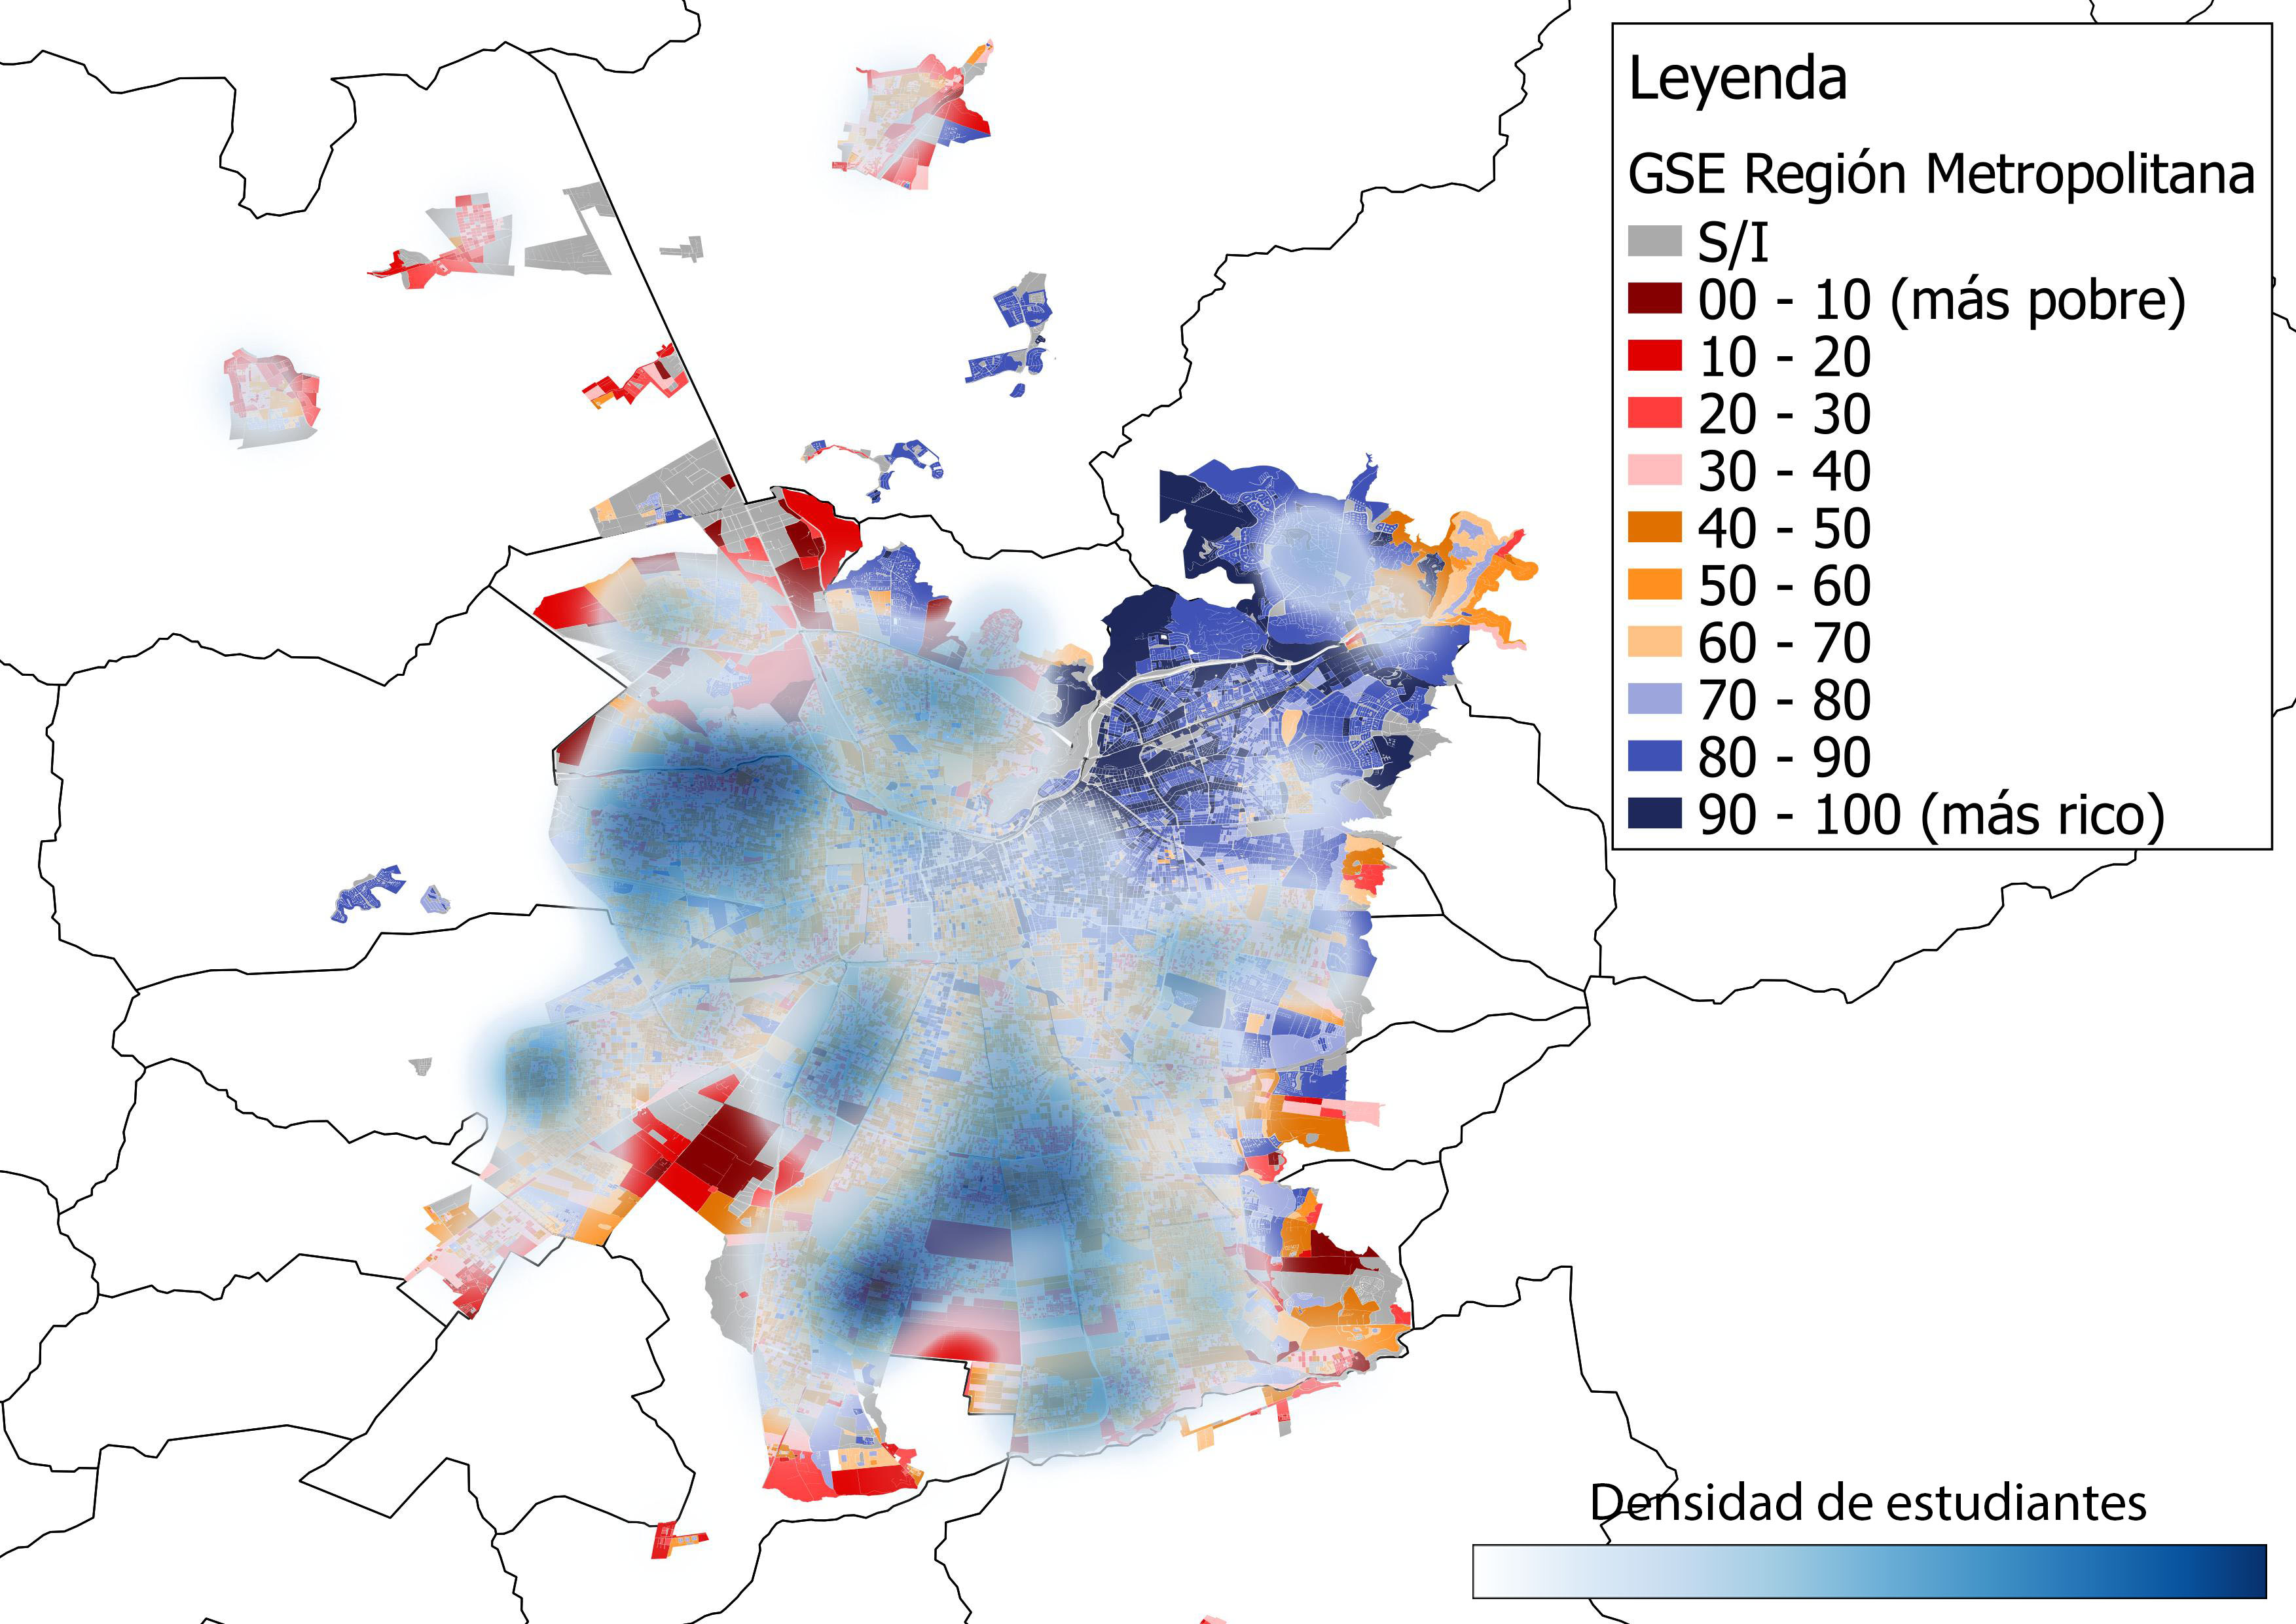
\includegraphics[width=7.5cm]{images/matriculas/M_CON_0_final.jpg}}
  \subfloat[Matrículas clúster M\_TODAS\_CON\_1.]{
   \label{f:}
    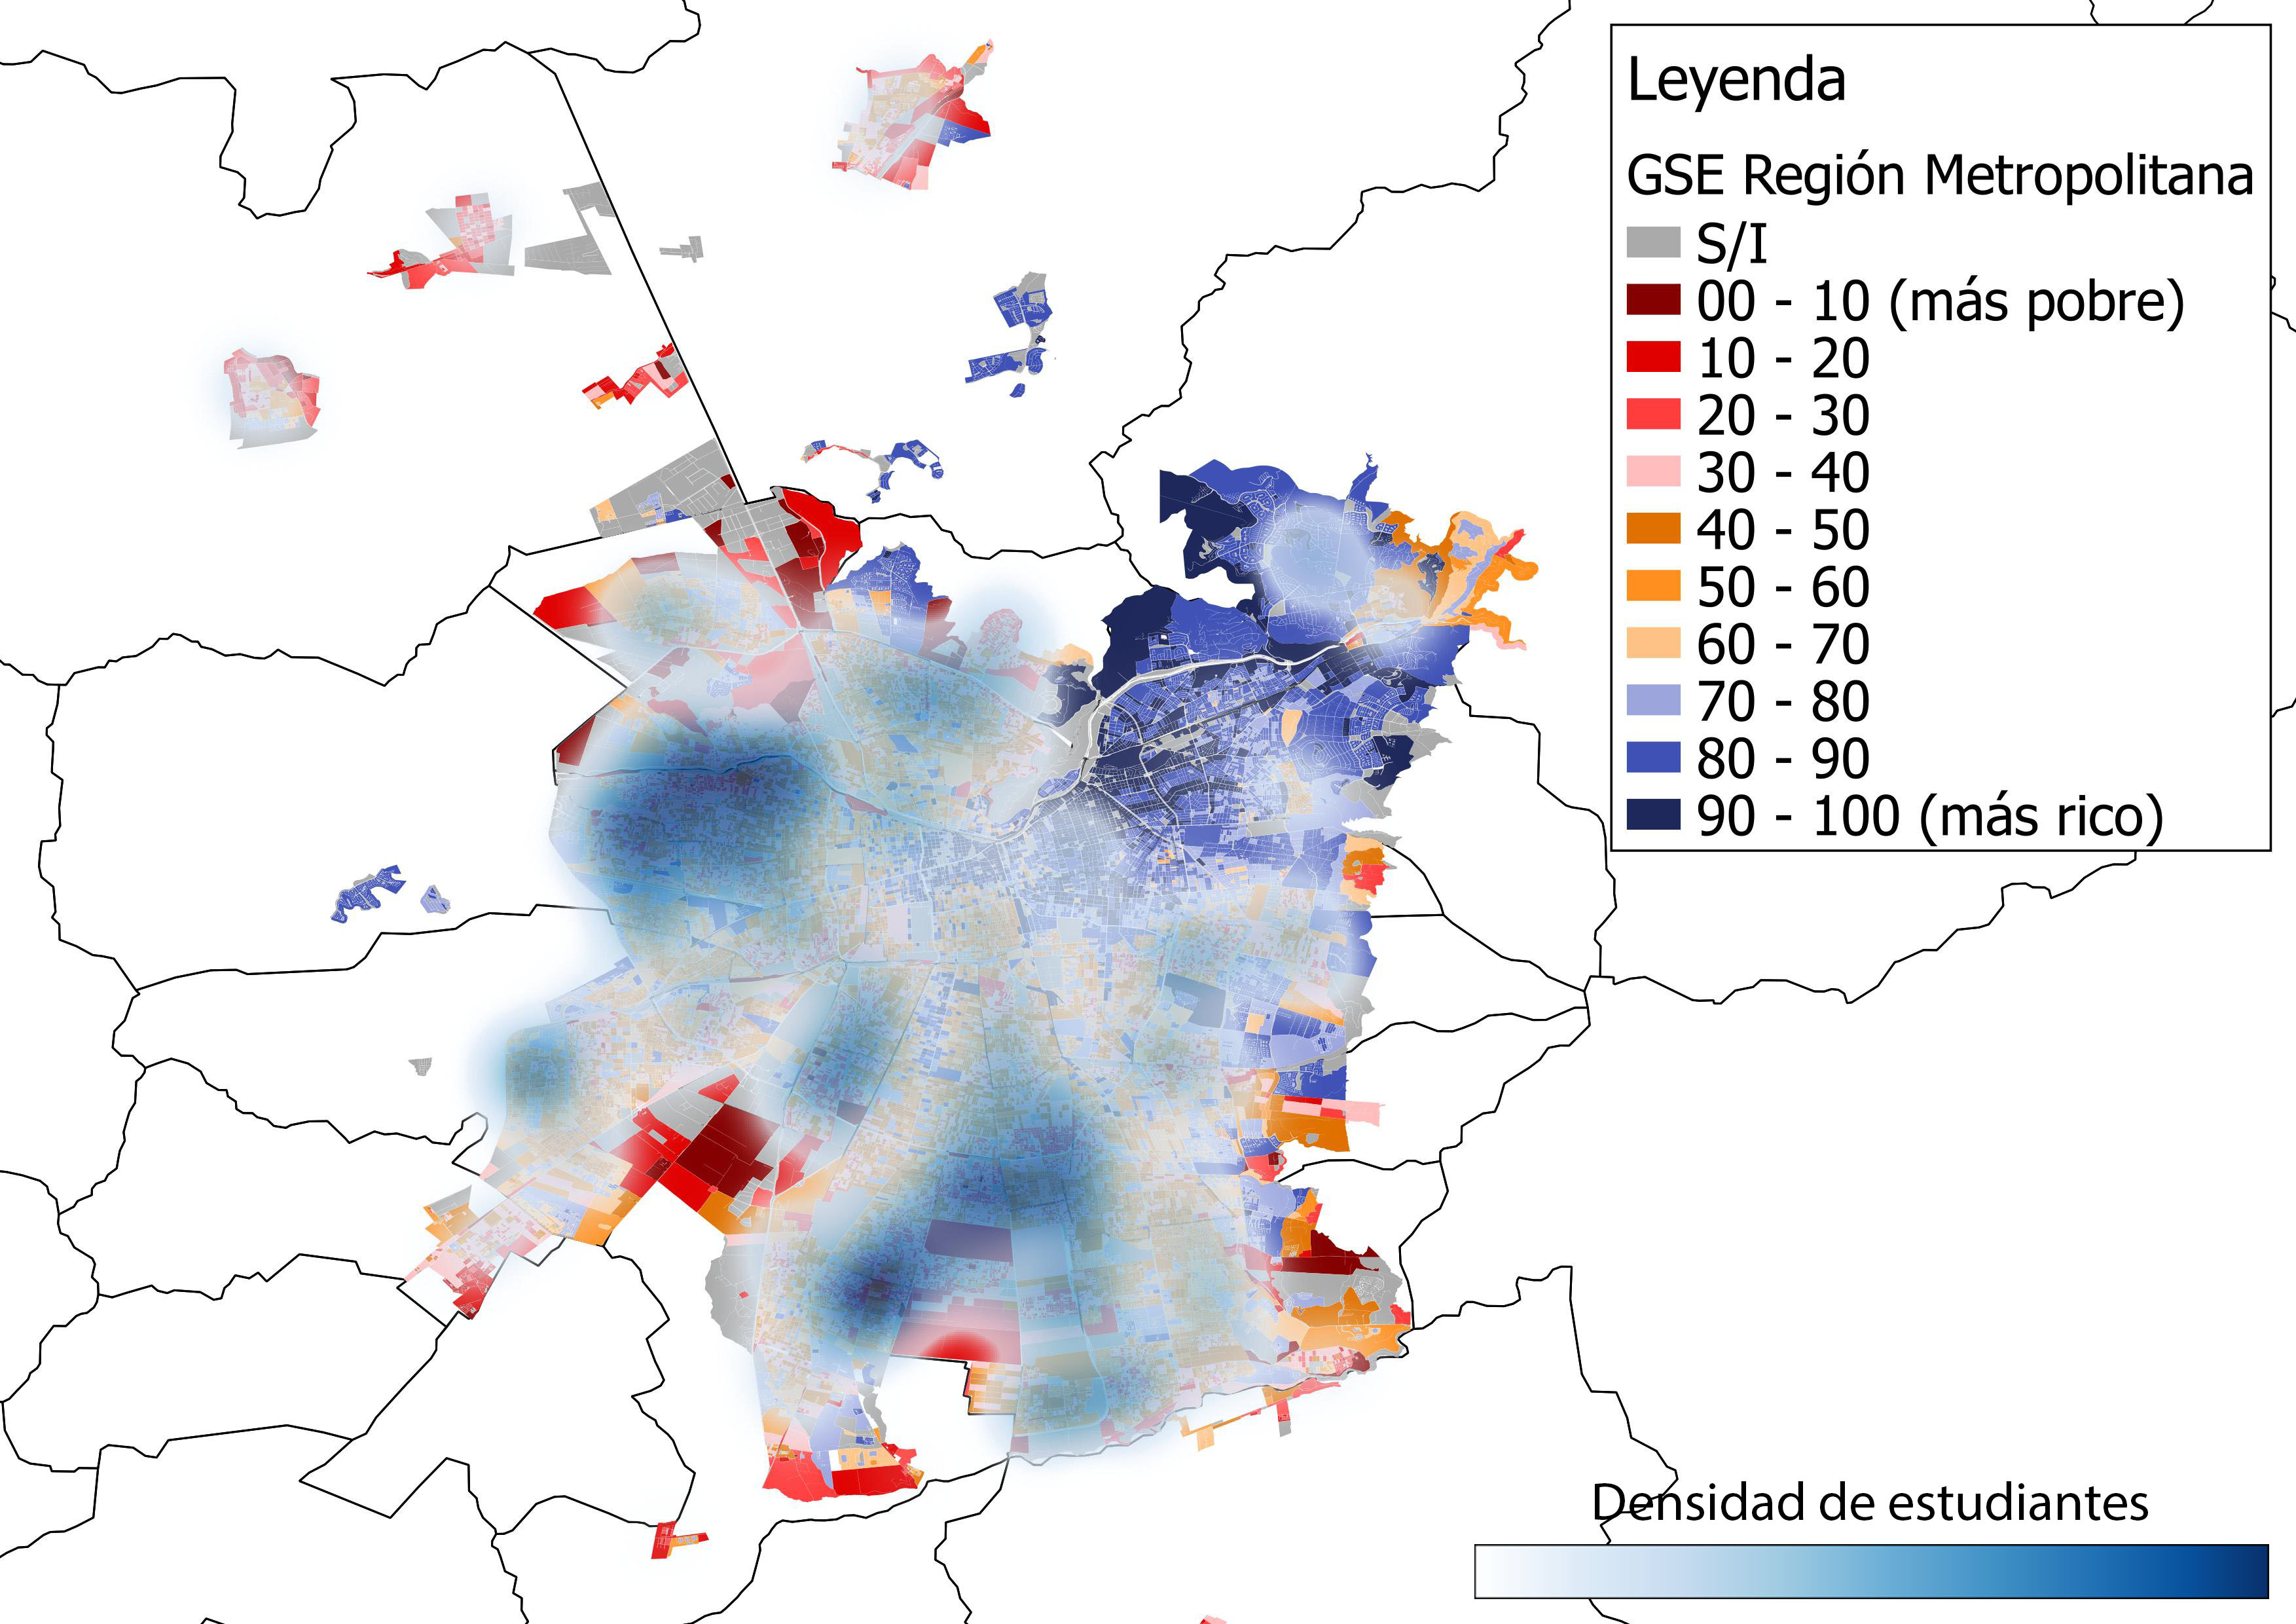
\includegraphics[width=7.5cm]{images/matriculas/M_CON_1_final.jpg}}\hspace{1mm}
  \subfloat[Matrículas clúster M\_TODAS\_CON\_2.]{
   \label{f:}
    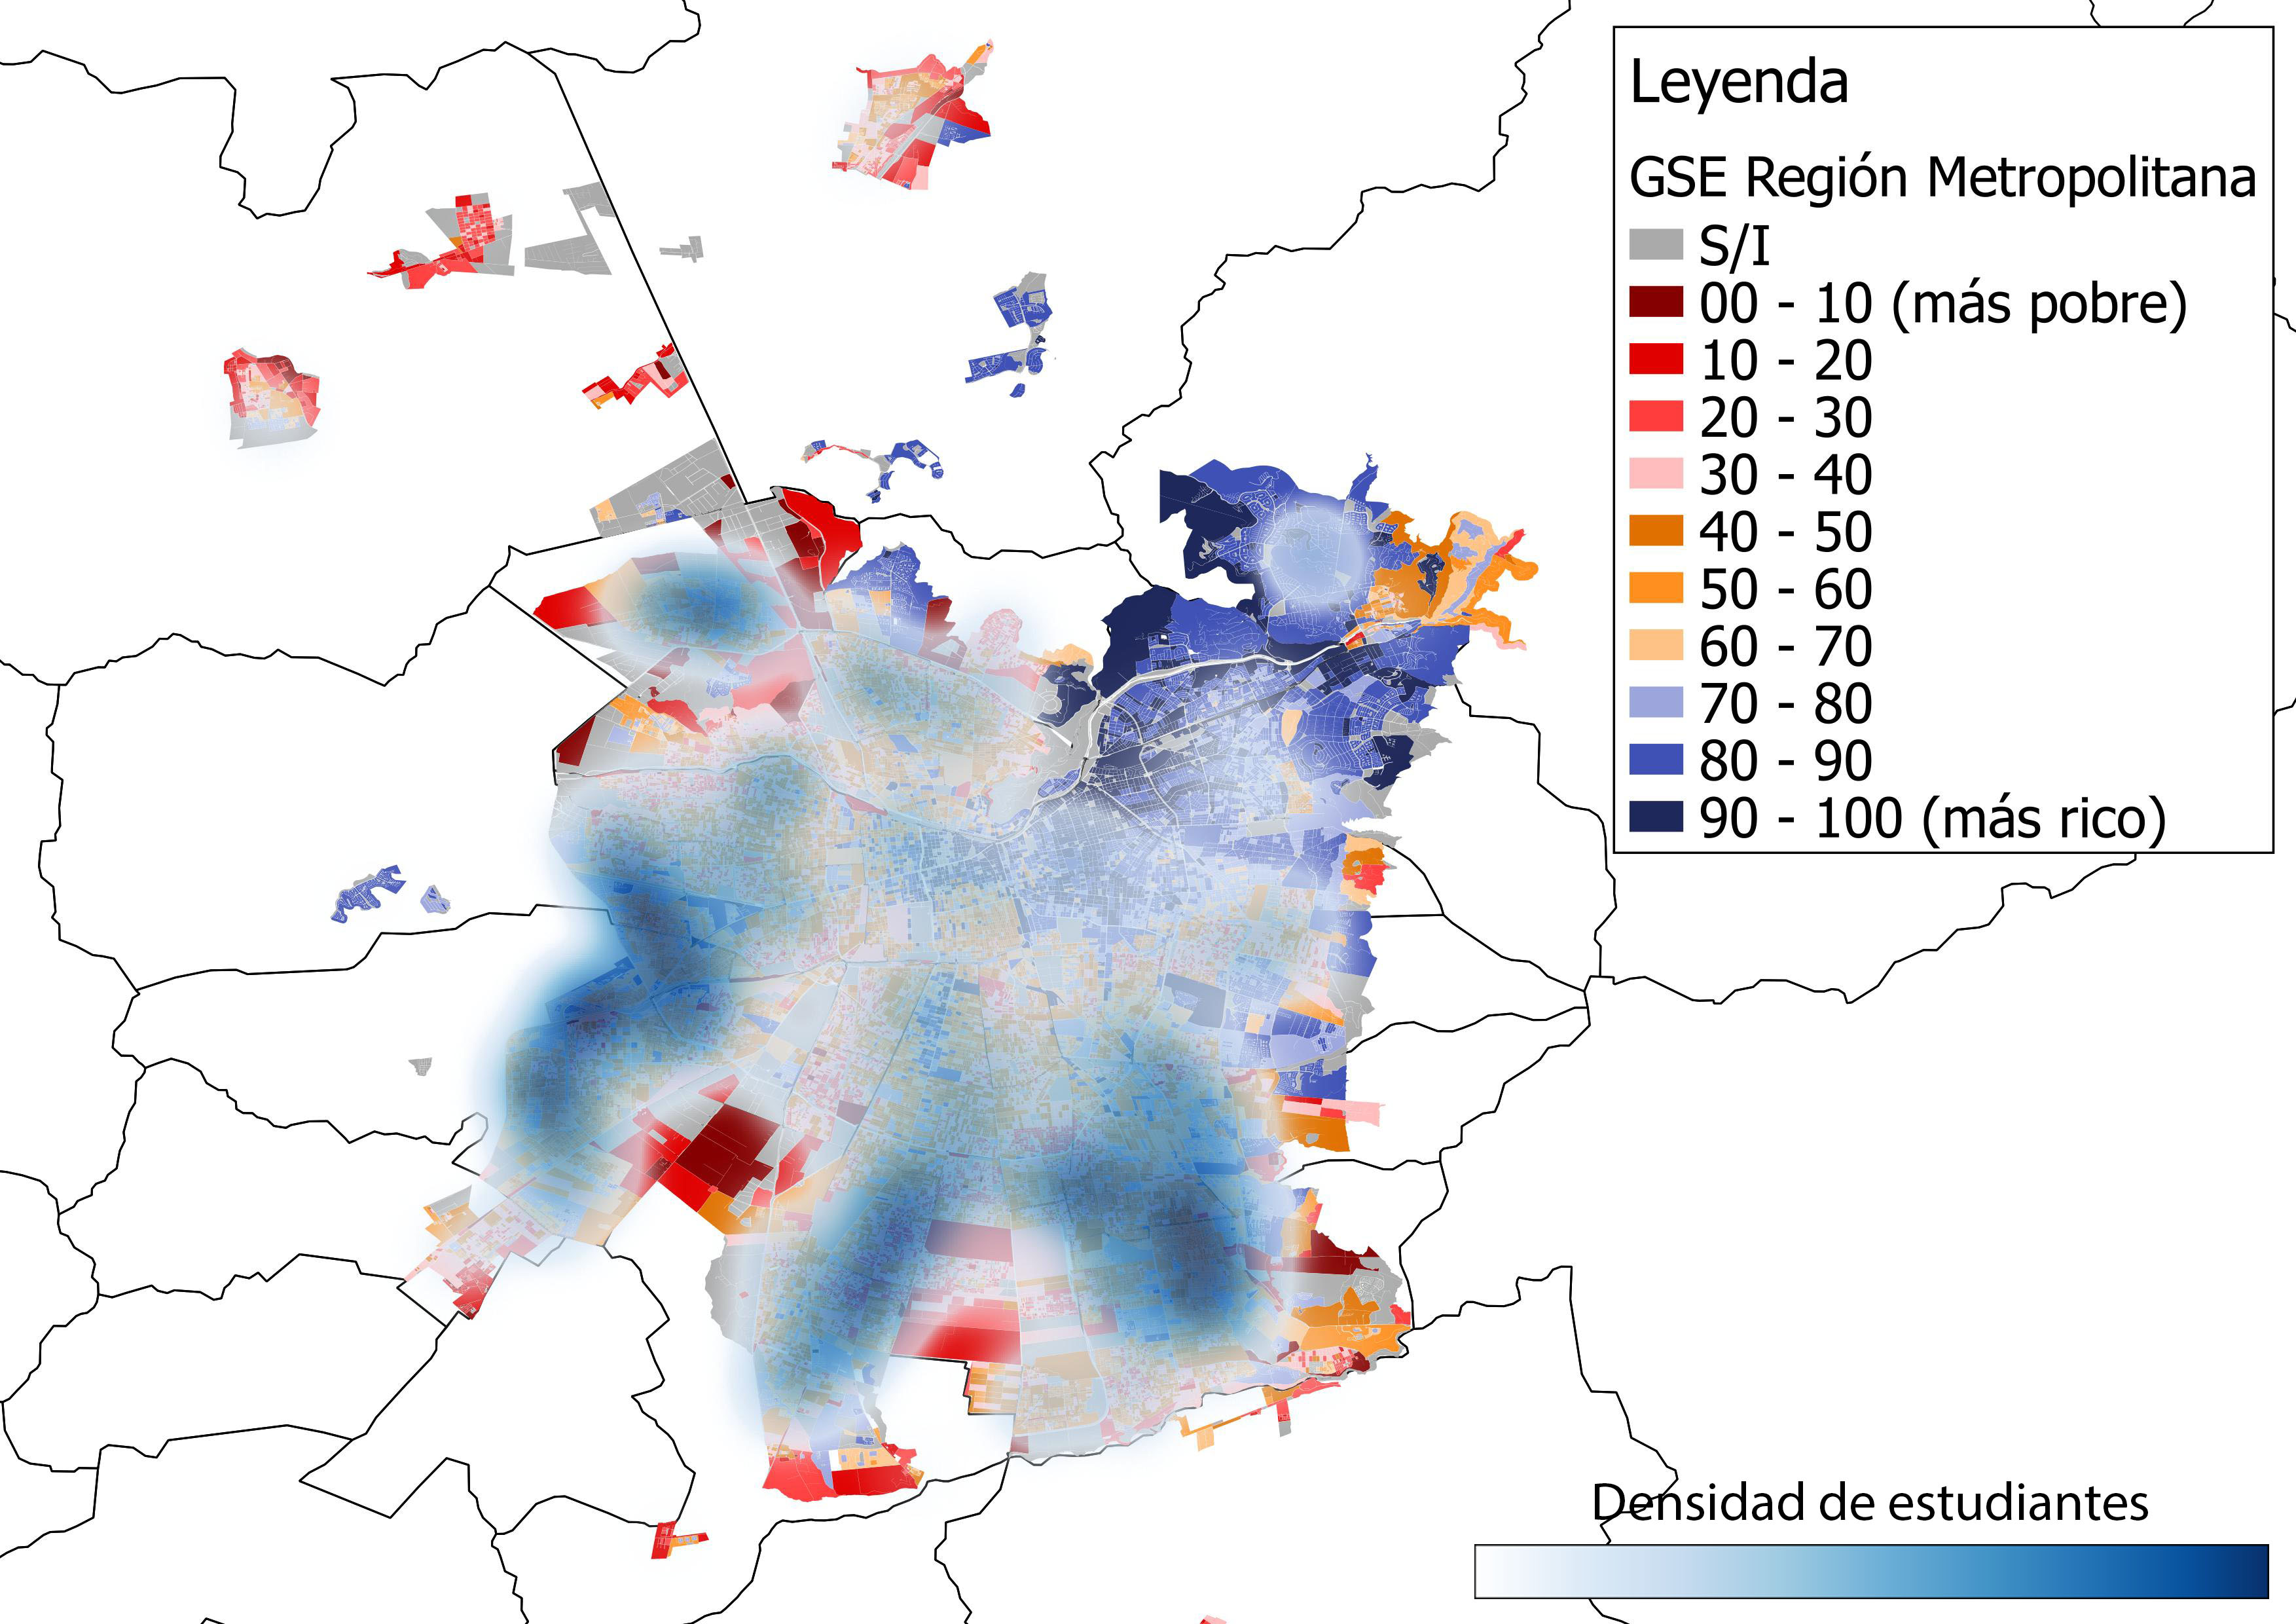
\includegraphics[width=7.5cm]{images/matriculas/M_CON_2_final.jpg}}
  \subfloat[Matrículas clúster M\_TODAS\_CON\_3.]{
   \label{f:}
    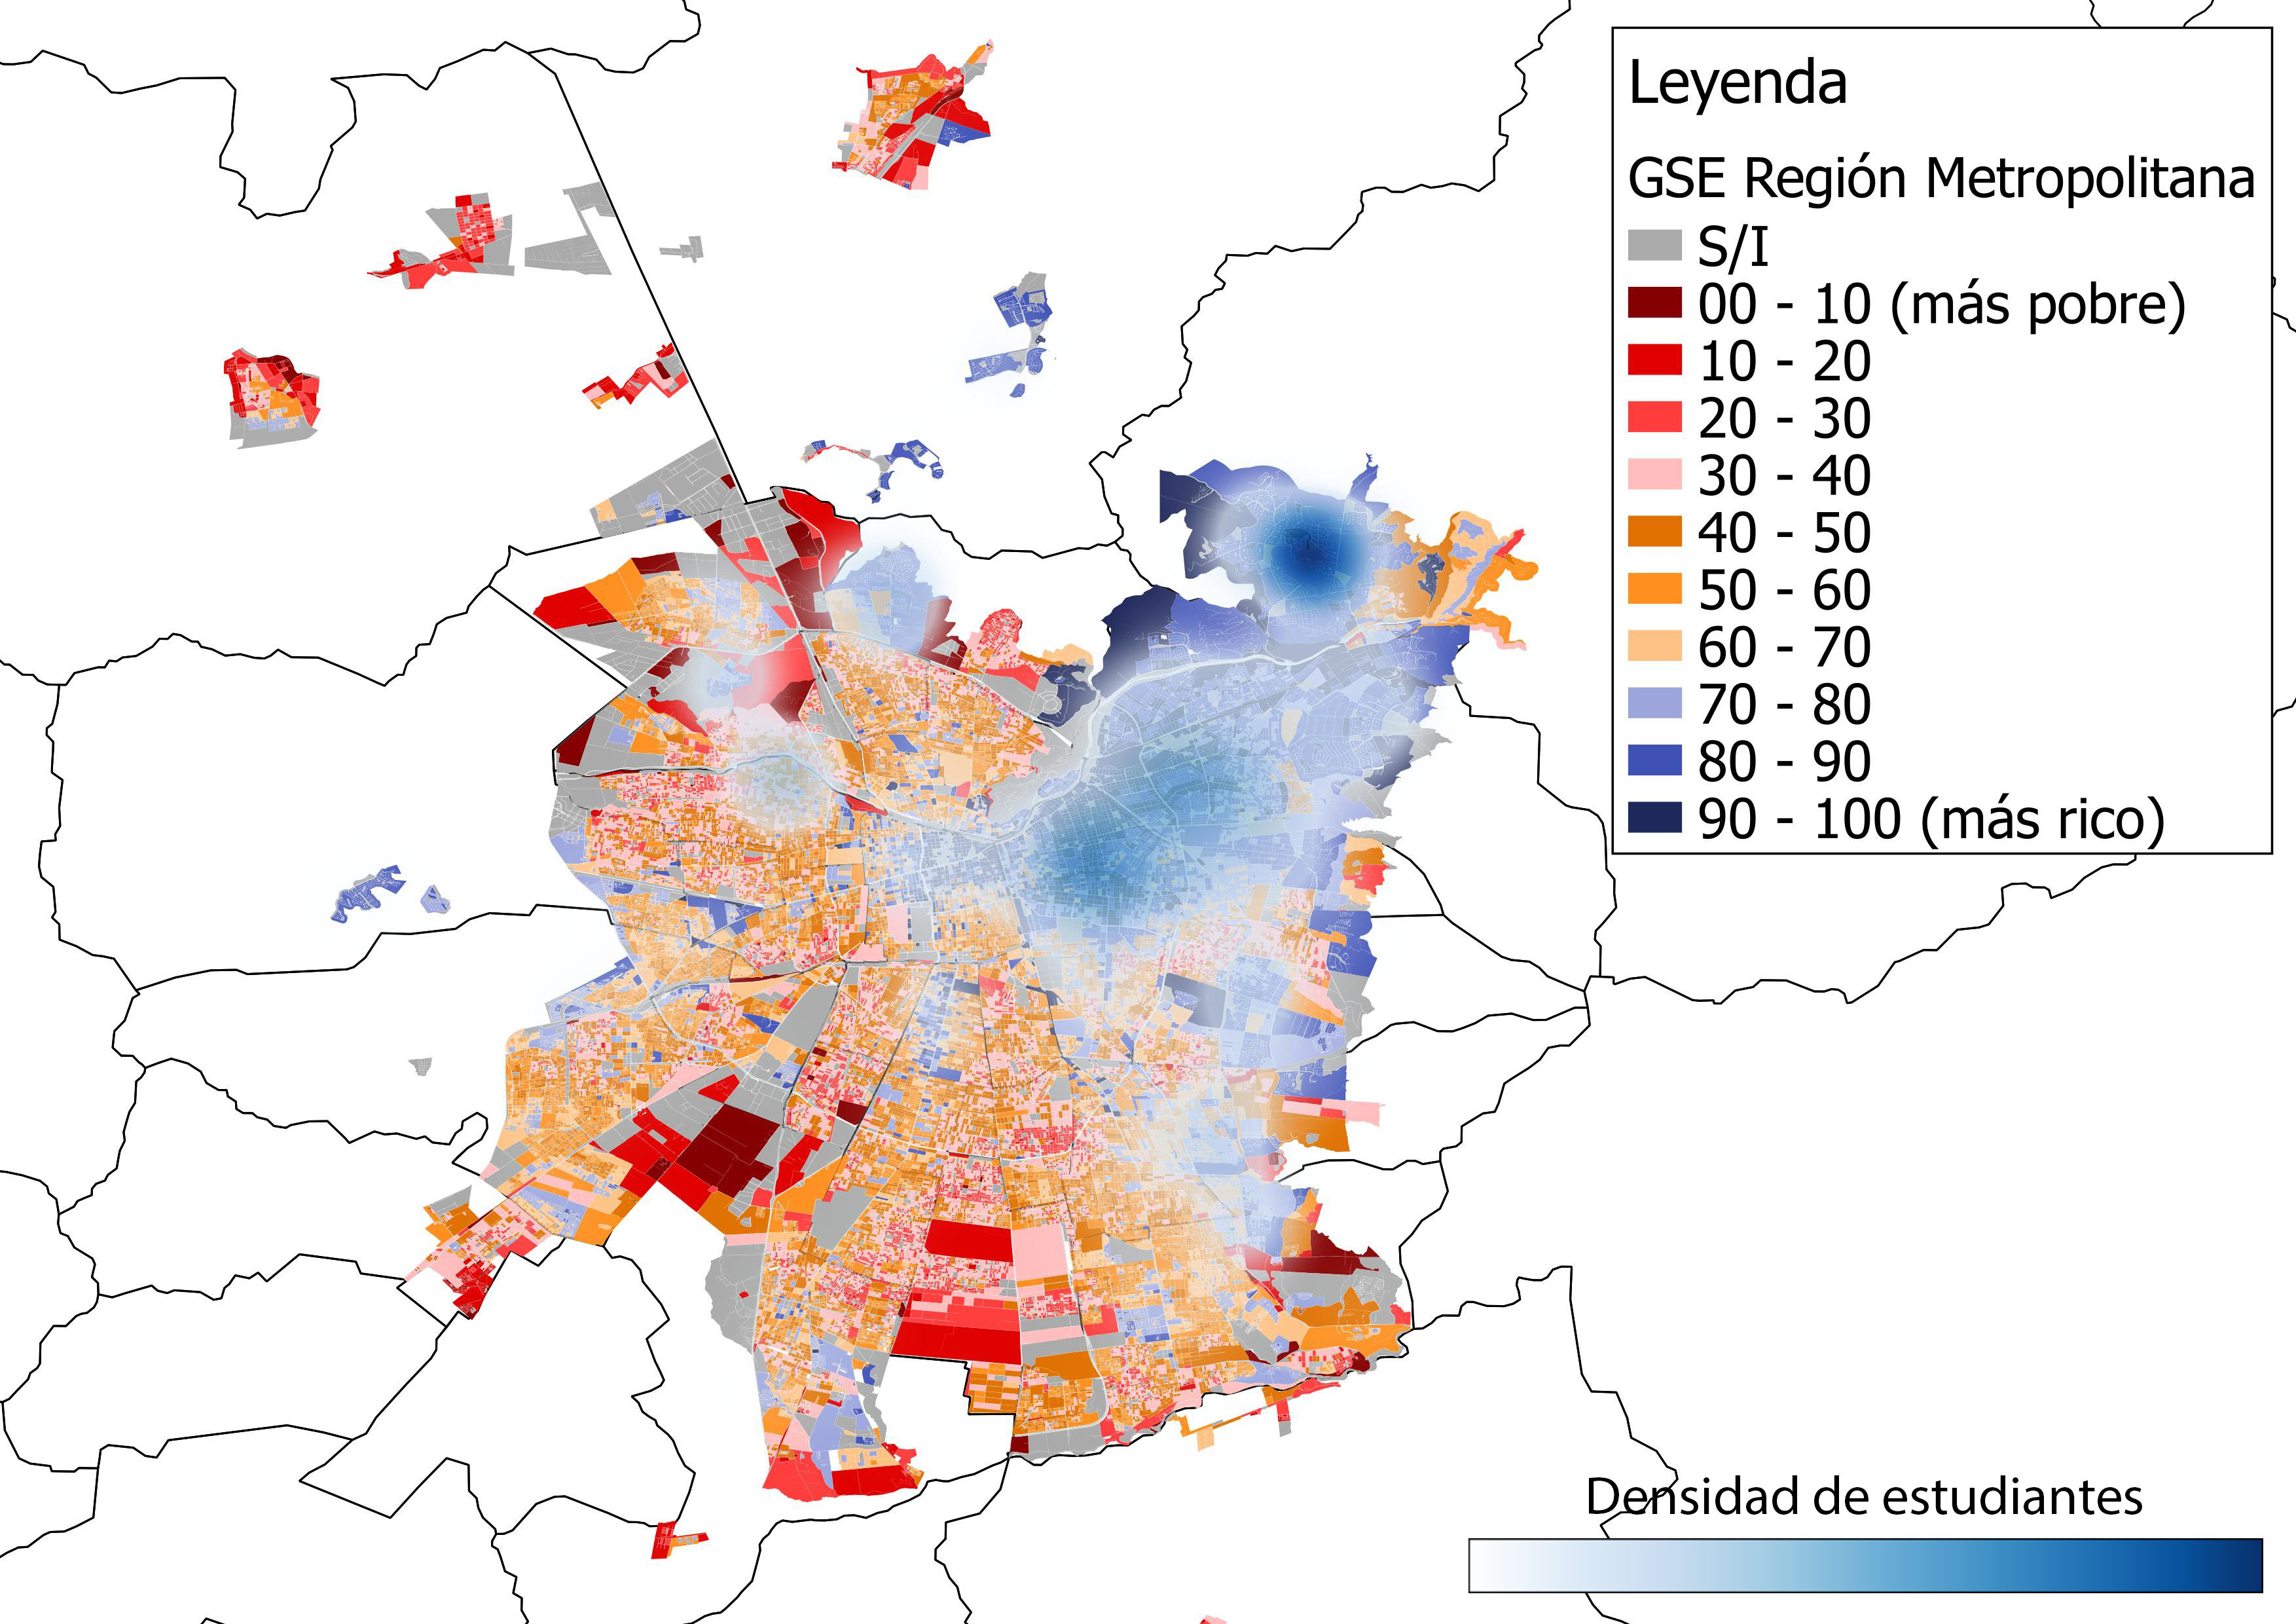
\includegraphics[width=7.5cm]{images/matriculas/M_CON_3_final.jpg}}
 \caption{Mapas de calor de clústers de matrículas (con atributos relacionales) sobre mapa GSE de la Región Metropolitana.}
 \label{f:}
\end{figure}

